% =====================================================================
%  main.tex — 主文件（Lead 独占）
%  编译：在 源码\ 目录下 `xelatex main.tex` 两遍（或用 ..\工程文件\build.ps1）
% =====================================================================
\documentclass[UTF8,a4paper,11pt]{ctexart}
% =====================================================================
%  src/preamble.tex  —  导言区
%  由 Lead 维护；队友只读。若缺宏，在文末「追加区」补 \newcommand，
%  并在回报中列出新增宏名（不得改动上面的已有定义）。
% =====================================================================
\usepackage[a4paper,margin=2.6cm,top=3.0cm,bottom=2.8cm]{geometry}
\usepackage{amsmath,amssymb,amsthm,mathtools,amscd}
\usepackage{mathrsfs}
\usepackage{graphicx}
\usepackage{array,booktabs,longtable}
\usepackage{caption}
\usepackage{enumitem}
\usepackage{xcolor}
\usepackage{fancyhdr}
\usepackage{tikz-cd}   % 交换图（原文若有）

% ---------- 字体（Windows，显式路径，不依赖 fontconfig） ----------
\setCJKmainfont[Path=C:/Windows/Fonts/,BoldFont=simhei.ttf,ItalicFont=simkai.ttf]{simsun.ttc}
\setCJKsansfont[Path=C:/Windows/Fonts/]{simhei.ttf}
\setCJKmonofont[Path=C:/Windows/Fonts/]{simfang.ttf}
\setCJKfamilyfont{zhkai}[Path=C:/Windows/Fonts/]{simkai.ttf}
\setCJKfamilyfont{zhhei}[Path=C:/Windows/Fonts/]{simhei.ttf}
\setCJKfamilyfont{zhfang}[Path=C:/Windows/Fonts/]{simfang.ttf}
\providecommand{\kaishu}{\CJKfamily{zhkai}}
\providecommand{\heiti}{\CJKfamily{zhhei}}
\providecommand{\fangsong}{\CJKfamily{zhfang}}

% ---------- 数学宏（只用这些，禁止在块文件里自造） ----------
\newcommand{\dd}{\mathrm{d}}
\newcommand{\ee}{\mathrm{e}}
\newcommand{\ii}{\mathrm{i}}
\DeclareMathOperator{\Tr}{Tr}
\DeclareMathOperator{\Aut}{Aut}
\DeclareMathOperator{\id}{id}
\DeclareMathOperator{\ind}{ind}
\DeclareMathOperator{\Ham}{Ham}
\DeclareMathOperator{\Hilb}{Hilb}
\DeclareMathOperator{\Vect}{Vect}
\DeclareMathOperator{\Alg}{Alg}
\DeclareMathOperator{\sHam}{sHam}
\DeclareMathOperator{\SQM}{SQM}
\DeclareMathOperator{\QM}{QM}
\DeclareMathOperator{\QFT}{QFT}
\DeclareMathOperator{\qft}{qft}
\DeclareMathOperator{\sqft}{sqft}
\DeclareMathOperator{\EBord}{EBord}
\DeclareMathOperator{\Bord}{Bord}
\DeclareMathOperator{\Rep}{Rep}
\DeclareMathOperator{\Th}{Th}
\DeclareMathOperator{\BPU}{BPU}
\DeclareMathOperator{\MP}{MP}
\DeclareMathOperator{\Spec}{Spec}
\newcommand{\TMF}{\mathrm{TMF}}
\newcommand{\tmf}{\mathrm{tmf}}
\newcommand{\KO}{\mathrm{KO}}
\newcommand{\KR}{\mathrm{KR}}
\newcommand{\MU}{\mathrm{MU}}
\newcommand{\MSpin}{\mathrm{MSpin}}
\newcommand{\MString}{\mathrm{MString}}
\newcommand{\R}{\mathbb{R}}
\newcommand{\C}{\mathbb{C}}
\newcommand{\Z}{\mathbb{Z}}
\newcommand{\Q}{\mathbb{Q}}
\newcommand{\N}{\mathbb{N}}
\newcommand{\PP}{\mathbb{P}}
\newcommand{\HH}{\mathbb{H}}
\newcommand{\cA}{\mathcal{A}}
\newcommand{\cB}{\mathcal{B}}
\newcommand{\cC}{\mathcal{C}}
\newcommand{\cD}{\mathcal{D}}
\newcommand{\cE}{\mathcal{E}}
\newcommand{\cF}{\mathcal{F}}
\newcommand{\cG}{\mathcal{G}}
\newcommand{\cH}{\mathcal{H}}
\newcommand{\cL}{\mathcal{L}}
\newcommand{\cM}{\mathcal{M}}
\newcommand{\cN}{\mathcal{N}}
\newcommand{\cO}{\mathcal{O}}
\newcommand{\cP}{\mathcal{P}}
\newcommand{\cS}{\mathcal{S}}
\newcommand{\cU}{\mathcal{U}}
\newcommand{\cV}{\mathcal{V}}
\newcommand{\cX}{\mathcal{X}}
\newcommand{\Ho}{H^{\bullet}}
\newcommand{\eps}{\varepsilon}
\newcommand{\ol}[1]{\overline{#1}}
\newcommand{\figomit}[2]{\par\smallskip\noindent\begingroup\small\kaishu\color{gray}〔原文图 #1 从略：#2〕\endgroup\par\smallskip}

% ---------- 定理类环境（编号一律手工给：\begin{definition}[2.1]） ----------
\theoremstyle{definition}
\newtheorem*{definition}{定义}
\newtheorem*{example}{例}
\newtheorem*{exercise}{习题}
\newtheorem*{conjecture}{猜想}
\newtheorem*{hypothesis}{假设}
\newtheorem*{question}{问题}
% 中文正文不用 plain 斜体：定理/命题/推论/引理一律直立（definition 风格）
\theoremstyle{definition}
\newtheorem*{theorem}{定理}
\newtheorem*{proposition}{命题}
\newtheorem*{corollary}{推论}
\newtheorem*{lemma}{引理}
\theoremstyle{remark}
\newtheorem*{remark}{注}

% 让 \begin{definition}[2.1] 印成「定义 2.1」
\makeatletter
\def\thmhead@plain#1#2#3{%
  \thmname{#1}\thmnumber{\@ifnotempty{#2}{ #2}}%
  \thmnote{\@ifnotempty{#3}{\hspace{0.35em}#3}}}
\let\thmhead\thmhead@plain
\makeatother

% ---------- 版式 ----------
\setlength{\parindent}{2em}
\linespread{1.18}
% 中文与公式混排行内偶有难以断行的长串：给足紧急伸长量，避免 Overfull
\setlength{\emergencystretch}{2em}
\setlist{nosep,leftmargin=2.2em}
\renewcommand{\arraystretch}{1.15}

\pagestyle{fancy}
\fancyhf{}
\fancyhead[L]{\small\kaishu 椭圆上同调与量子场论}
\fancyhead[R]{\small\thepage}
\renewcommand{\headrulewidth}{0.4pt}
\fancypagestyle{plain}{\fancyhf{}\fancyfoot[C]{\small\thepage}\renewcommand{\headrulewidth}{0pt}}

\ctexset{
  section = {
    format = \Large\bfseries\heiti,
    beforeskip = 2.2ex plus 1ex minus .2ex,
    afterskip  = 1.4ex plus .2ex,
    name = {},
    number = \arabic{section},
  },
  subsection = {
    format = \large\bfseries\heiti,
    beforeskip = 1.8ex plus .6ex minus .2ex,
    afterskip  = 1.0ex plus .2ex,
  },
}

% 超链接（必须放最后）
\usepackage[hidelinks,bookmarksnumbered=false,bookmarksopen=true,
            pdftitle={椭圆上同调与量子场论（中文译注本）},
            pdfauthor={Daniel Berwick-Evans}]{hyperref}
\pdfstringdefDisableCommands{\def\ol#1{#1}}

% ===================== 追加区（队友可 append \newcommand） =====================


\begin{document}

% ---------------------------- 封面 ----------------------------
\begin{titlepage}
\centering
\vspace*{3.2cm}
{\heiti\zihao{2} 椭圆上同调与量子场论\par}
\vspace{1.2cm}
{\kaishu\zihao{3} Elliptic Cohomology and Quantum Field Theory\par}
\vspace{2.2cm}
{\zihao{4} Daniel Berwick-Evans\par}
\vspace{0.6cm}
{\zihao{5} Department of Mathematics, University of Illinois Urbana-Champaign\par}
\vspace{2.4cm}
{\kaishu\zihao{4} 中文译注本\par}
\vspace{0.8cm}
{\zihao{5} 底本：arXiv:2408.07693v1 [math.AT]，2024 年 8 月 14 日，34 页\par}
\vspace{0.5cm}
{\zihao{5} 原文首页不编号注（作者致谢 NSF 资助 DMS-2205835、DMS-2340239）\par}
\vfill
{\kaishu\zihao{5}
本译注本依据 arXiv:2408.07693v1 全文翻译。原文全部 56 条编号公式与全部编号\\
猜想/定义/注/例/定理/命题/推论/假设均与原文逐一对应；原文 8 幅插图不复刻，\\
仅在原位置保留图注译文与「图从略」标记；原文笔误照译，并以注释指出正确形式。\par}
\vspace{1.0cm}
\end{titlepage}

% ---------------------------- 目录 ----------------------------
\tableofcontents
\newpage

% ------------------------- 译者说明（可后写） -------------------------
% translator_note.tex — 译者说明（放在目录之后、正文之前）
% 4–6 段中文；体例说明见 STYLE_GUIDE.md
\section*{译者说明}
\addcontentsline{toc}{section}{译者说明}

一、底本。本译注本依据 Daniel Berwick-Evans（University of Illinois Urbana-Champaign 数学系）的综述 \textit{Elliptic Cohomology and Quantum Field Theory}（arXiv:2408.07693v1 [math.AT]，2024 年 8 月 14 日，34 页）全文译出。原文是一篇导引性的综述章节（原文自称 chapter），目标是把「椭圆上同调的上闭链即二维超对称场论」这一猜想（原文猜想 1.1）拆解为可操作的分析数据与配边数据，并用大量例子说明其来源与后果。译文保持原文的章节结构与论证顺序，不作改写、删节或补充；原文的段落划分、脚注位置与文献引用标记一仍其旧。

二、编号。原文全文的编号公式构成单一序列 (1)–(56)，本译本逐条保留原编号，以 \verb|\tag| 手工排出，与原文严格一一对应。原文的编号环境（猜想、定义、注、例、命题、定理、推论、假设）在同一节内共享计数器，本译本同样按原文号手工排出，不重排、不跳号；原文中带括号说明的条目（如「定义 1.5（[ST11, Definition 5.2] 之略述）」），译文亦保留该说明。正文引用一律写作「式 (12)」「猜想 1.1」「定义 2.13」这类形式，不使用 \verb|\eqref|，以便与原文的纸质阅读顺序一致。原文公式编号排在页面左侧边栏，译本沿用中文数学书的通行体例排在右侧。

三、图与表。原文的 8 幅插图（Figure 1–8）均不复刻，只在原位置保留「图从略」标记与图注译文，正文中「见图 3」一类指引照译。交换图与显示公式以 LaTeX 重排：能写成配边三角形、自然变换方块的一律按原样排出，2-胞之类无法用 CD 环境表达的图形用简化的 TikZ 图重排，其顶点、边与标签与原文一一对应。原文正文提到的 Table 2 在原文中并无对应实体表格，译文照译并在源码批注中说明。

四、批注。源码中以 \% [Tutor Note: …] 形式保留了 Tutor Note 批注，内容限于四类：可验证的易错点、原文省略论证的补充、原文笔误、记号说明。批注不进入排版成品，只随源码交付。凡原文确有的笔误，译文一律照原文排印，另在批注中指出正确形式，并在工程文件目录下的 ERRATA.md 中登记；可疑而不能确定的写法只加批注、不改动原文，以免以译者之见覆盖作者原意。原文的脚注共 9 处，译文用 LaTeX 自动编号，个别处与原文序号不同者已在批注中注明；原文首页不编号的作者单位与 NSF 资助说明（DMS-2205835、DMS-2340239）移至封面。

五、术语。术语以工程文件目录下的 glossary.tsv 冻结表为准（共 151 条），同一英文术语全文用同一中文译名。人名、理论名、软件名与文献标签不音译：Witten、Stolz、Teichner、Segal、Hopkins、Lurie、Atiyah–Singer、Quillen、Ochanine、TMF、K-theory、Spin、string、Ramond、Neveu–Schwarz、Wick 等保留拉丁字母。表外的新术语在首次出现处写作「中文（English）」，并已回填该表。数学表述以原文页面图像为唯一依据（原文 PDF 的文字层会把分式压成一行、把矩阵拆成单字符），每条编号公式均经放大核对，不凭文字层转写。

六、致谢与免责。本译本仅供学习与研究之用，著作权归原作者 Daniel Berwick-Evans 所有；译文中的任何错误与不当表述均由译者负责，欢迎指正。感谢原作者写下这篇清晰而慷慨的综述，也感谢 Stolz 与 Teichner 的框架（原文 [ST11]）为本译本的术语选择提供了依据。


% ---------------------------- 正文 ----------------------------
% 每节另页起（书籍常规排版）
\clearpage
\section{引言}
% sec1.tex — c01｜原文 p1–5（并含 p6 上半的 §1.4–§1.5，即 §1 全文）｜§1 引言
% 公式号 (1)–(5)；编号环境 1.1–1.12
% 块边界：c02 从 p6 的「2. The homotopy type of quantum mechanics」标题开始，不重复本块 §1.4–§1.5。

% [原文 p.1]
20 世纪 80 年代后期，Witten 利用理论物理的方法构造了一个取值于整模形式的椭圆亏格 [Wit88a]。他的论证暗示，椭圆上同调与量子场论之间存在深得多的联系。沿着这些想法，Segal 把 2 维量子场论精确地定义为配边范畴的一个射影表示 [Seg04]。同一时期，Hopkins 及其合作者发展了椭圆上同调这一课题，其顶点是拓扑模形式（TMF）的构造，以及把 Witten 亏格提升为环谱之映射的 string 定向 [Hop02, Lur09b]。经过跨越数十年的种种洞见与努力，一幅把 TMF 与场论的几何联系起来的丰富图景正在浮现。在 Stolz 与 Teichner 的框架中，基本猜想可概述如下 [ST11]。

\begin{conjecture}[1.1]
对每个 $n\in\Z$ 与光滑流形 $X$，存在虚线箭头
\begin{equation}
\begin{tikzpicture}[baseline=(current bounding box.center), >=stealth]
  \node (A) at (0,3.6) {$\left\{\begin{array}{c}\text{一族 $n$ 维 string 流形}\\[2pt] \text{$M\to X$}\end{array}\right\}$};
  \node (C) at (8.4,1.8) {$\TMF^{-n}(X)$};
  \node (B) at (0,0) {$\left\{\begin{array}{c}\text{全扩张的、次数为 $-n$ 的}\\[2pt] \text{2 维超对称场论}\\[2pt] \text{（定义在 $X$ 上）}\end{array}\right\}$};
  \draw[->] (A.south east) -- node[above, sloped] {拓扑指标} (C.north west);
  \draw[->, dashed] (A.south) -- node[left] {量子化} (B.north);
  \draw[->, dashed] (B.east) -- node[below right=1pt, pos=0.42] {上闭链${}_{-n}$} (C.south west);
\end{tikzpicture}
\tag{1}
\end{equation}
使三角形交换；其中“拓扑指标”是 string 定向，“量子化”是对 $M\to X$ 的纤维上的超对称 $\sigma$ 模型作量子化，“上闭链$_n$”把 $X$ 上次数为 $n$ 的场论送到 $\TMF^n(X)$ 中的一个类。当 $n$ 为负时，空流形是唯一的 string 流形，此时 (1) 的内容是存在一个上闭链映射。
\end{conjecture}
% [Tutor Note: 式 (1) 中“拓扑指标”那条箭头在原文画作实线，另两条为虚线，而正文统称 "dashed arrows"；照译。实线表示 string 定向这一已知映射，虚线才是待构造的部分。]
% [Tutor Note: 式 (1) 的箭头标签是 $\mathrm{cocycle}_{-n}$（下标带负号），而紧邻的正文写作 cocycle$_n$；二者不矛盾：三角形针对 degree $-n$ 的场论，故下标随度数变号。]

简言之，猜想 1.1 提出 TMF 的一种几何构造，其上闭链是 2 维量子场论。它还提出一个 TMF-指标定理：当 $n\ge 0$ 时，虚线箭头的复合定义一个解析指标，而三角形 (1) 把它与 Ando–Hopkins–Rezk 构造的拓扑指标等同起来 [AHR10]。Stolz 与 Teichner 已经解释了这一被提议的 TMF-指标定理如何推广 Atiyah 与 Singer 的指标定理 [ST04]；见下文猜想 3.1。
% [Tutor Note: 原文 p1 底部另有一条不编号的注（作者单位与 NSF 资助 DMS-2205835、DMS-2340239），译本把它移入封面，以保持正文脚注编号与原文一致（本块即原文脚注 1、2）。]

% [原文 p.2]
\subsection{猜想为何有趣}
拓扑 K 理论在 20 世纪数学中的核心地位，来自它与诸多学科相互交织的方式。在几何中，向量丛决定 K 理论类。在分析中，Fredholm 算子空间表示 K 理论。在代数中，紧 Lie 群的表示决定（等变的）K 理论类。许多重要结果都依赖于这些相互联系，其中 Atiyah–Singer 指标定理是沟通分析、几何与拓扑的登峰造极之例。在代数拓扑内部，TMF 比 K 理论深刻得多，例如 $\pi_*\TMF$ 探测到球面稳定同伦群中多得多的类。然而，几何描述的缺失在很大程度上把 TMF 的触角限制在同伦理论的领域内。解决猜想 1.1 将改变这一局面。

与来自代数拓扑的这一动机互补，理论物理当前的一个主题是理解各种量子场论的空间，包括 string 理论中的景观问题 [Sus07, Dou10] 与物质的拓扑相 [Kit09a, FM13]。猜想 1.1 断言，其中一个这样的量子场论空间具有非常有趣的拓扑。所讨论的量子理论在 2 维具有最小超对称；这给可观测量施加的约束相对贫乏，使得标准计算变得困难。在假定猜想 1.1 成立的前提下所作的物理推理，已经产生了一连串令人惊讶的预言，其中许多又与数学相联系，例如参见 [GJF23, GPPV21, Tac21, TY23b, TY23a, TYY23, LP23]。举两个具体例子：TMF 中丰富的挠元指示出量子场论的新形变不变量，它们细化椭圆亏格 [GJFW21]；TMF 的 576 周期性则预言了手征自由费米子中一个令人惊讶的周期性 [DH11]。总而言之，人们期待解决猜想 1.1 将为研究一般的量子场论空间提供重要的数学工具，并特别地给出对 2 维场论与 string 理论结构的深刻洞察 [Wit88a]。

人们还期待 (1) 在同伦理论与理论物理之外的应用。下面强调三个方面。

在微分几何中，Stolz 猜想 Witten 亏格是正 Ricci 曲率度量存在的障碍 [Sto96]。正标量曲率的类似障碍，即 $\hat{A}$-亏格障碍，使用的是 Dirac 算子的几何 [Lic63]。与此相关，Hopkins 勾勒了如何通过 signature 算子的一个 TMF 推广来探测自由环路空间上的异种光滑结构 [DFHH14, 第 10 章]，这一推广由 Witten 提议 [Wit88a]。若不能牢牢把握 (1) 中场论的几何，这类环路空间指标理论仍将遥不可及。

在代数中，格顶点算子代数可以编码散在群，最著名的是通过 Borcherd's 对魔群月光猜想的证明 [Bor92]。
% [Tutor Note: 原文 p2 写作 "Borcherd's proof"，应为 "Borcherds' proof"（Richard Borcherds，1992 年证明 monstrous moonshine）；按“笔误照排”处理，已登记 ERRATA。]
格的 $\theta$ 函数也决定一个拓扑模形式 [Hop02, §5]。人们期待 (1) 中的上闭链映射能澄清围绕魔群、2 维共形场论与椭圆上同调的这些巧合及其他巧合 [Mor09, JF20, Lin22, AKL23]。

在表示论中，Grojnowski 描述了由等变上同调与等变 K 理论构成的标准例子的椭圆推广 [Gro07]。用复解析等变椭圆上同调（粗略地说，等变的 $\TMF\otimes\C$）推进这些想法，已经引出一些极其丰富的对象 [GKV95, ZZ15, YZ17, FRV17, RTV17, AO21, RSVZ22, GR13, KRW19, RW20, RW22]。
% [Tutor Note: 原文 p2 写 "has lead to"，应为 "has led to"；中文无形态变化，照译，已登记 ERRATA。]
% [Tutor Note: “等变的 $\TMF\otimes\C$” 指复化（complexification），而非给 TMF 增加新的张量结构；原文以 “roughly” 限定。]
在这些构造中——与 K 理论和普通上同调形成对照——相应的等变椭圆上同调类并没有被很好理解的几何描述。相应地，这些“椭圆主题”的代数的真正起源仍有些晦暗不明。对 (1) 的更好理解似乎必然会为这些深刻的对象提供进一步的洞见，例如通过整性细化。

\begin{remark}[1.2]
猜想 1.1 有一个重要的加强版本，它断言：$X$ 上次数为 $n$ 的场论的 concordance 类与 $\TMF^n(X)$ 一一对应。换言之，TMF 是 2 维超对称场论的完全形变不变量。这严格地难于猜想 1.1，并引入笔者希望在本综述中回避的技术性细节。简短的讨论参见下文注 3.21。
\end{remark}
% [Tutor Note: concordance 是场论之间的一种等价关系（沿超区间族的同伦），比猜想 1.1 的“存在上闭链”强得多；本译保留原文 concordance 并附中文“协调类”。]

% [原文 p.3]
\subsection{超对称量子场论的框架}
数学量子场论中一个反复出现的主题是算子代数分析与时空几何之间的相互作用。例如，Jones 的贡献——经 Witten 进一步放大——利用量子场论在纽结的几何与 von Neumann 代数的分析之间锻造出深刻的联系 [Jon87, Wit89, Ati90]。人们期待猜想 1.1 将沿着这条道路继续。Atiyah [Ati89] 与 Segal [Seg04] 提供了一种考察几何与分析之交界的富有影响力的语言：一个 $d$ 维量子场论是从 $d$ 维配边范畴到拓扑向量空间的对称幺半函子，
\begin{equation}
(\Bord_d,\bigsqcup)\longrightarrow(\Vect,\otimes).
\tag{2}
\end{equation}
几何位于 (2) 的源中，泛函分析位于其目标中。例如在 2 维，源可以选取得以捕捉 Riemann 面的模空间（如 Segal 关于共形场论的原始工作），目标可以选取得以编码核 Fréchet 空间在射影张量积下的分析。
% [Tutor Note: 式 (2) 的源范畴用不交并 $\bigsqcup$ 作幺半结构、目标用张量积 $\otimes$；这正是“配边→向量空间”的函子成为对称幺半函子的条件。]

除 (2) 之外，如今关于数学量子场论有许多流派，各自为 (1) 带来自己的洞见，例如顶点代数 [GMS00, HK04, GL22]、因子化代数 [Cos10, GG14] 与共形网 [Was98, BDH15]。归根结底，这些语言中每一种的发展，以及比较它们的“词典”的发展，都将加快猜想 1.1 以及数学量子场论中其他未决问题的进展。为了具体起见，下文将遵循 Stolz 与 Teichner [ST11]，通过 (2) 的视角考察猜想 1.1。

首先，对一个刚性几何 $\mathcal G$ 与一个光滑叠 $\cX$，存在 $\cX$ 上带 $\mathcal G$-结构的配边的对称幺半范畴 $\Bord_{\mathcal G}(\cX)$ [ST11, Definitions 2.21, 2.46, 2.48, and 4.4]。配边是定义量子场论所在的时空或世界面，叠 $\cX$ 则贡献背景场。在猜想 1.1 的情形中，背景场就是到光滑流形 $X$ 的映射。但允许更一般的背景场（例如带联络的 $G$-丛，即背景规范场）将是重要的。

下面两类例子可以让人对范畴 $\Bord_{\mathcal G}(\cX)$ 有所体会。

\begin{example}[1.3（欧几里得配边范畴）]
一个原型性的刚性几何是 $\R^d$ 上的平坦 spin 几何，其特征是等距群 $\R^d\rtimes\mathrm{Spin}(d)$ 通过平移与保向旋转（经由二重覆盖 $\mathrm{Spin}(d)\to\mathrm{SO}(d)$）作用在 $\R^n$ 上。此时记相应的 $\cX$ 上 $d$ 维欧几里得配边范畴为 $\EBord_d(\cX)$。$\EBord_d(\cX)$ 中的态射（记作 $\Phi\colon\Sigma\to\cX$）是带平坦度量与测地边界的紧 spin $d$-流形 $\Sigma$，连同映射 $\Phi\colon\Sigma\to\cX$。配边的源与目标来自把 $\Phi$ 限制到边界的一个划分 $\partial\Sigma=\partial_{\mathrm{in}}\Sigma\sqcup\partial_{\mathrm{out}}\Sigma$ 上，分为入射（源）与出射（目标）两部分。\footnote{为简洁起见，定义中省略了几个重要的技术细节。例如，为使 $\EBord_d$ 中的复合有良好定义，要求 $\partial_{\mathrm{in}}\Sigma$ 与 $\partial_{\mathrm{out}}\Sigma$ 具有领（collar）。细节参见 [ST11]。}
\end{example}
% [Tutor Note: 例 1.3 中刚性几何定义在 $\R^d$ 上，而等距群却写作作用在 $\R^n$ 上；原文如此（沿用 ST11 的记法，$n$ 记环境维数），此处应读作 $n=d$，照排不改。]

\begin{example}[1.4（超欧几里得配边范畴）]
把例 1.3 加以推广，超欧几里得刚性几何决定配边范畴 $\EBord_{d|\delta}(\cX)$，它依赖于一对自然数 $d|\delta$（即一个超维数）以及附加数据 [ST11, §4.2]。粗略地说，$\EBord_{d|\delta}(\cX)$ 中的态射仍是带平坦度量与测地边界的紧 spin $d$-流形 $\Sigma$，连同映射 $\Phi\colon\Sigma\to\cX$。新特征是：$\delta$ 维复旋量丛 $S\to\Sigma$ 被视为“奇的”，而超对称是 $S\to\Sigma$ 的自同构，它们把 $\Sigma$ 中的偶方向与 $S$ 中的奇方向混合起来。粗略到一阶近似，$\EBord_{d|\delta}(\cX)$ 就是 $\EBord_d(\cX)$ 再加上这些奇自同构。要把这一点说精确，需要超流形的语言 [Fre99, DM99]。
\end{example}

由此得到我们对超对称场论的第一个概念（后文还会展开）。

% [原文 p.4]
\begin{definition}[{1.5（[ST11, Definition 5.2] 之略述）}]
以 $\Alg$ 记 $\Z/2$-分次拓扑代数、双模与双模映射构成的 2-范畴，其对称幺半结构来自 $\Z/2$-分次张量积。光滑叠 $\cX$ 上的扭 $d|\delta$ 维超对称欧几里得场论是一个自然变换 $E$
\begin{equation}
\begin{tikzpicture}[baseline=(current bounding box.center), >=stealth]
  \node (A) at (0,0) {$\EBord_{d|\delta}(\cX)$};
  \node (C) at (7.6,0) {$\Alg$};
  \draw[->] (A) to[bend left=30] node[above] {$\mathbf 1$} (C);
  \draw[->] (A) to[bend right=30] node[below] {$\alpha$} (C);
  \node at (3.8,0) {$E\ \Downarrow$};
\end{tikzpicture}
\tag{3}
\end{equation}
介于常值函子 $\mathbf 1$（取值于 $\Alg$ 的幺半单位）与称为扭的函子 $\alpha$ 之间。$\cX$ 上的扭场论是一个群胚的对象。
\end{definition}
% [Tutor Note: 定义 1.5 中的 $\mathbf 1$ 是取值为 $\Alg$ 幺半单位的常值函子，不是数字 1；式 (3) 中 $E$ 是自然变换 $\mathbf 1\Rightarrow\alpha$，2-胞的上下两条 1-态射分别是 $\mathbf 1$ 与 $\alpha$。]

对定义的若干结构方面作些说明。第一，场论对 $\cX$ 是自然的：对映射 $\cX\to\cX'$，显然的函子 $\EBord(\cX)\to\EBord(\cX')$ 诱导出从 $\cX'$ 上的扭场论到 $\cX$ 上的扭场论的拉回。第二，扭与扭场论有乘法：$\Alg$ 上的幺半结构给出
\[
(E\colon\mathbf 1\Rightarrow\alpha,\ E'\colon\mathbf 1\Rightarrow\alpha')\ \overset{\otimes}{\longmapsto}\ (E\otimes E'\colon\mathbf 1\simeq\mathbf 1\otimes\mathbf 1\Rightarrow\alpha\otimes\alpha').
\]
扭 $\alpha$ 称为可逆的，若存在扭 $\alpha'$ 以及与平凡扭的等价 $\alpha\otimes\alpha'\simeq\mathbf 1$。下文考虑的所有扭都是可逆的。

可逆扭是刻画反常量子场论的一种方式 [Fre14]。粗略地说，射影对称性决定反常，而扭场论是配边范畴的射影表示。定义 1.5 的各种变体已在文献中出现（常常是独立出现的），例如 Freed 与 Teleman 的相对场论 [FT14]。Stolz 与 Teichner 所选的术语，来自反常量子场论与扭上同调类之间一个发展中的联系 [Sto19]。

\begin{remark}[1.6]
提请注意：定义 1.5 中的扭与 [Wit91] 中的拓扑扭无关，例如镜像对称中的 A-扭与 B-扭 [Wit88b]。
\end{remark}

\begin{example}[1.7（非扭场论）]
以 $\Vect$ 记 $\C$ 上 $\Z/2$-分次（拓扑）向量空间带张量积构成的对称幺半范畴。非扭场论是对称幺半函子 $\EBord_{d|\delta}(\cX)\to\Vect$，它给出平凡扭 $\alpha=\mathbf 1$ 下的自然变换 (3) [ST11, Lemma 5.7]。

扭的数据的一部分，是对每个对象 $Y\in\EBord_{d|\delta}(\cX)$ 的一个代数 $\alpha(Y)$；扭场论的数据的一部分，是一个左 $\alpha(Y)$-模 $E(Y)$。这样，扭场论可以看作取值于 $\alpha(Y)$-模（而非向量空间）的非扭场论；参见 [ST11, page 52]。
\end{example}

\begin{example}[1.8（次数扭）]
在定义 1.5 中取 $d|\delta=1|1$ 与 $2|1$，则对每个 $n\in\Z$ 存在一个次数扭 [ST11, §5.3]（另见下文定义 3.18 与 4.15）
\begin{equation}
\mathrm{EBord}_{d|1}(\mathrm{pt})\xrightarrow{\ \alpha_n\ }\Alg,
\qquad \alpha_n\otimes\alpha_m\simeq\alpha_{n+m},
\qquad n,m\in\Z,\ d\in\{1,2\}.
\tag{4}
\end{equation}
当 $d=1$ 时，第 $n$ 个次数扭由第 $n$ 个 Clifford 代数 $\mathrm{Cl}_n$ 决定，见式 (37)。当 $d=2$ 时，它由 $n$ 个（手征）自由费米子决定，其中包括无穷维 Clifford 代数 $\mathrm{Cl}(L\R^n)$ 的数据，其中 $L\R^n$ 是 $\R^n$ 的自由环路空间，见式 (54)。
\end{example}
% [Tutor Note: 次数扭只对 $d|1$（$d=1,2$）定义；$d=2$ 时由 $n$ 个手征自由费米子给出，涉及 $L\R^n$ 上的无穷维 Clifford 代数，对应式 (54)。]

为准确捕捉所期望的例子，我们给扭场论增添一种附加的结构与性质，称为反射正性。简言之，这是关于扭与扭场论的 $\Z/2$-等变数据，相对于配边上反转定向的对合，以及由 $\C$ 上复共轭给出的 $\Alg$ 上的对合。相对于这些等变数据，理论中的 Hermite 配对被要求是内积。综述性讨论见 [FH21, §3] 或 [KS21, page 18]。在定义 1.5 的语境下，反射正性的完整定义仍在发展之中；一个可用的定义出现在 [BE23c, §C.3] 中，我们在下文定义 2.13 中勾勒相关特征。
% [Tutor Note: 反射正性的等变数据含两处对合：配边上的定向反转、$\Alg$ 上由复共轭诱导的对合；二者作用后 Hermite 配对须为正定内积。]

% [原文 p.5]
\begin{definition}[1.9]
以 $\QFT^{\alpha}_{d|\delta}(\cX)$ 记如下群胚：其对象是 $\cX$ 上反射正的 $\alpha$-扭 $d|\delta$ 维欧几里得场论，其态射是与反射结构相容的扭场论的同构。
\end{definition}

\begin{definition}[1.10]
对 $n\in\Z$ 与光滑叠 $\cX$，以
\[
\QFT^{n}_{d|1}(\cX):=\QFT^{\alpha_n}_{d|1}(\cX)
\]
记由 (4) 沿映射 $\cX\to\mathrm{pt}$ 的拉回所扭的场论构成的范畴。
\end{definition}

特别地取光滑流形 $\cX=X$ 时，范畴 $\QFT^{n}_{d|1}(X)$ 是猜想 1.1 中所期望的对象的最著名近似。
% [Tutor Note: 原文此处写 "Specializing to a smooth manifold X = X"，其中前一个 X 实为叠 $\cX$；原文记号混用，照译作 $\cX=X$。]
% [Tutor Note: 原文 "and (at present) it unclear which one to take" 缺系动词，应为 "it is unclear"；照译，已登记 ERRATA。]
但若要对证明该猜想抱有任何希望，还需要进一步的修改：切除要求全扩张的场论，见 [ST11, Conjecture 1.17] 与 [ST04, §1]。这一向下扩张的过程需要超欧几里得配边的 2-范畴，以及把 $\Alg$ 去环（deloop）的 3-范畴。定义 1.9 并未唯一确定源范畴或目标范畴。相反，存在大量的推广，而（目前）尚不清楚该取哪一个。

\subsection{用 Lurie 的高阶范畴等变性加强猜想}
缩小可能定义之“动物园”的一条途径，是在猜想 1.1 中要求更多结构。这使人更难猜出“错误”的场论定义。一个有希望的选择是 Lurie 的高阶范畴等变椭圆上同调，在 [Lur09b, §5] 中称为 2-等变椭圆上同调。它对每个紧 Lie 群 $G$ 给出一个导出概形 $\cM_G$，对每个级别 $[\ell]\in H^4(BG;\Z)$ 给出 $\cM_G$ 上的线丛 $\cL_\ell$。$\cM_G$ 底层的普通概形是椭圆曲线上平坦 $G$-丛的模空间，$\cL_\ell$ 底层的普通线丛以非 Abel $\theta$ 函数为截面。正如导出椭圆曲线模叠上函数层的整体截面给出 TMF，$\cL_\ell$ 在 $\cM_G$ 上的整体截面决定 2-等变 TMF，记作 $\TMF^{\ell}_{G}$ [Lur19, GM23]。

紧 Lie 群 $G$ 作用在流形 $X$ 上决定叠 $\cX=X/\!/^{\nabla}G$，\footnote{栈 $X/\!/^{\nabla}G$ 分类带联络的 $G$-丛 $(P,\nabla)$ 以及 $G$-等变映射 $P\to X$。丢弃联络数据给出遗忘函子 $X/\!/^{\nabla}G\to X/\!/G$，打到通常的商栈。}从而给出猜想 1.1 的 $G$-等变加细，比较 [ST11, §1.7]。
% [Tutor Note: $X/\!/^{\nabla}G$ 中的 $\nabla$ 表示保留联络数据；忘掉联络即得通常的商叠 $X/\!/G$。这是本文“背景规范场”的几何来源。]

\begin{conjecture}[1.11]
对作用在流形 $X$ 上的紧 Lie 群 $G$ 与级别 $[\ell]\in H^4(BG;\Z)$，存在推广 (1) 的上闭链映射
\begin{equation}
\begin{tikzpicture}[baseline=(current bounding box.center), >=stealth]
  \node (A) at (0,0) {$\QFT^{\ell}_{2|1}(X/\!/^{\nabla}G)$};
  \node (C) at (8.2,0) {$\TMF^{\ell}_{G}(X)$};
  \draw[->, dashed] (A) -- node[above] {上闭链} (C);
\end{tikzpicture}
\tag{5}
\end{equation}
取值于 $X$ 的 $\ell$-扭 $G$-等变 TMF。此外，对 $G$-等变 string 流形的族，存在交换三角形 (1) 的类似物。
\end{conjecture}

用物理的语言说，范畴 $\QFT^{\ell}_{2|1}(\mathrm{pt}/\!/^{\nabla}G)$ 包含带有背景规范场与指定 't Hooft 反常的场论。由一般理论 [Fre87]，这样的反常决定亏格 1 曲面（即椭圆曲线）上 $G$-丛的模空间上的线丛。这些线丛是 Grojnowski 扭复解析等变椭圆上同调的核心 [Gro07, GKV95]。初步的研究表明，$\mathrm{pt}/\!/^{\nabla}G$ 上的扭欧几里得场论决定这类线丛的截面 [BET21, BET19]。因此，在与 Lurie 框架比较时，人们期待 $\QFT^{1}(-/\!/^{\nabla}G)$ 编码导出概形 $\cM_G$，而 $\QFT^{\ell}(-/\!/^{\nabla}G)$ 编码 $\theta$-线丛的截面 $\Gamma(\cM_G,\cL_\ell)$。

除了限制全扩张场论的可能定义之外，猜想 1.11 还照亮了构造场论与 TMF 之间比较映射的一条路径：Lurie 勾勒了 2-等变椭圆上同调的一个泛性质 [Lur09b, §5.5]。猜想 1.11 为场论提出一种 2-等变结构，于是 Lurie 的泛性质将引出所期望的比较映射。这样，高阶等变性可以看作开启猜想 1.1 的关键要素。

\begin{remark}[1.12]
等变椭圆上同调与 2 维规范理论之间的联系并不新鲜。最早的想法或许属于 Grojnowski [Gro07] 与 Segal [Seg88, Theorem 5.3] [Seg07, Definition 2.4]，不过其他人也独立地发现了类似的平行关系。例如，环路空间上 Dirac 算子的 Witten 刚性定理可以用 $S^1$-等变椭圆上同调来理解 [BT89, Ros01, AB02, Ros03]；而对有限群，人们早已清楚 $G$-等变椭圆上同调与 string 理论中的扭扇区（twisted sectors）相关 [DHVW85, Seg88, Dev96, Dev98, HKR00, Mor06]。

% [原文 p.6]
环路群及其正能表示也同时出现在 2 维场论（例如 WZW 模型）与等变椭圆上同调中 [Liu96, Kit09b, FHT11b, Kit14, Gan14, Lue22]。等变性还引向自然的椭圆幂运算，它们与 string 理论的几何有明显联系 [DMVV97, And00, Gan07, Gan06, Gan09, Hua18, HS20, BBES22]。
\end{remark}

\subsection{免责声明与概览}
本章有两个主要目标：(i) 为猜想 1.1 提供动机与直观；(ii) 描述其验证中仍然存在的中心困难。这两个目标都要求理解来自理论物理的例子，例如 $\sigma$ 模型与自由费米子。不幸的是，把这些（部分构造出来的）例子塞进量子场论的数学框架，会引入许多技术性细节，它们往往掩盖更大的图景。为此，下文的每一节都从某种特设的（ad hoc）量子力学系统与量子场论定义开始，这些定义明确捕捉了物理文献中出现的分析数据。特别地，对超对称量子力学，一个理论的相关数据是完全无歧义的，例子也已被很好地理解。把这些特设定义与代数拓扑中的对象联系起来之后，我们把分析数据安置在范式 (3) 的语境中，作为配边范畴的表示的一部分。这个配边定义指向 2 维量子场论中的一些新结构，它们难以仅凭超对称量子力学的朴素推广而窥见。为强调这一数学框架仍在发展之中，我们把带有证明梗概的陈述标记为假设（Hypothesis）；所引文献表明，已有密切相关的陈述被证明，但带有我们在此不讨论的技术性告诫。我们期待任何合理的定义都应当使所述的假设成立，因此本论述也意在提供具体的路标，以检验所提出的（全扩张）定义是否走在正确的轨道上。

下面简要概述本章。第 2 节先从分析的视角介绍量子力学，再把其基本结构翻译到配边框架中。第 3 节对超对称量子力学重复这一做法，并勾勒猜想 1.1 的 K 理论变体的一个版本。第 4 节从把量子场论看作量子力学之推广的分析视角开始，再把这些结构翻译到配边框架中。这一框架引出关于猜想 1.1 最终内容的各种洞见。
% [Tutor Note: 原文 "translating these structure into the bordism framework" 中 these structure 应为 this structure；中文不受影响，已登记 ERRATA。]

全文中，$\cH$ 表示一个（固定的）无穷维可分复 Hilbert 空间。$\Z/2$-分次对象的所有张量积都是 $\Z/2$-分次张量积，其对称同构编码 Koszul 符号。
% [Tutor Note: $\Z/2$-分次张量积的对称同构含 Koszul 符号，即 $a\otimes b=(-1)^{|a||b|}b\otimes a$；这是全文一切“超”结构的统一约定。]

\subsection{致谢}
感谢 Emily Cliff、André Henriques、Theo Johnson-Freyd、Matthias Ludewig、Laura Murray、Nat Stapleton 与 Arnav Tripathy 的许多富有启发的交谈，这些想法在其中成形。也感谢 Theo Johnson-Freyd 与 Laura Murray 对先前草稿的反馈。Stephan Stolz 与 Peter Teichner 的影响怎么强调都不过分——感谢他们的诸多洞见与慷慨分享想法。


\clearpage
\section{量子力学的同伦型}
% sec2.tex — c02｜原文 p6–p12，并含 p13 上半的 §2 尾部（例 2.22 的式 (20) 及注 2.23、例 2.24）
% 公式号 (6)–(20)；编号环境 2.1–2.24
% 块边界：从 p6 底部 "2. The homotopy type of quantum mechanics" 标题下的正文起（\section 本体在 main.tex）；
% p6 顶部的 §1.4–§1.5 由 sec1.tex 完成，本块不重复。本块终于例 2.24（§2 结束），§3 的标题在 main.tex。

% [原文 p.6]
设 $M$ 是闭的定向 Riemann 流形。$M$ 上的经典力学研究路径 $x\colon I\to M$，其作用量泛函为 $S(x)=\frac{1}{2}\int_I\|\dot{x}\|\,dt$。$S$ 的临界点是 $M$ 中参数化的测地线。利用指数映射与度量，这样的测地线可以与 $M$ 的余切丛等同起来。辛流形 $T^{*}M$ 的量子化产生 $M$ 上的量子力学，例如参见 [BW97]。下文只要求量子化的两项基本输出：(i) 状态空间 $\cH=L^{2}(M)$，以及 (ii) 由 $M$ 上的拉普拉斯算子给出的哈密顿量 $H=\Delta$。在 Wick 转动后的量子力学中，$(\cH,H)$
% [Tutor Note: 此处 $S$ 是长度泛函（原文未平方），其临界点即参数化测地线；若改用能量泛函 $\frac12\int_I\|\dot{x}\|^{2}dt$，临界点是常速测地线。核对时勿按能量泛函自行补平方。]

% [原文 p.7]
确定半群 $(\R_{\ge 0},+)$ 的一个表示
\begin{equation}
\R_{\ge 0}\to\mathrm{End}(\cH),\qquad t\mapsto e^{-tH}
\tag{6}
\end{equation}
取值于 $\cH$ 上的自伴算子，且当 $t>0$ 时为迹类（这里用到 $M$ 的紧性）。这引出下面的定义，其精确表述将在下文 §2.1 给出。
% [Tutor Note: (6) 中 $e^{-tH}$ 与后文 (11) 的 $E(\mathrm{I}^{\pm}_t)=e^{-tH}$ 是同一个半群；$t>0$ 的迹类条件正是配分函数 $\Tr(e^{-tH})$（式 (11) 中 $E(S_t)$）收敛所需的，核对 (11) 第三行。]

\begin{definition}[2.1]
一个\emph{量子力学系统}是一个状态空间 $\cH$ 与一个哈密顿量 $H$，它们确定一个自伴的、迹类的表示 (6)。量子力学系统 $(\cH,H)$ 与 $(\cH',H')$ 称为\emph{等价的}，若存在酉映射 $u\colon\cH\to\cH'$ 使得 $H'=uHu^{-1}$。
\end{definition}
% [Tutor Note: 等价条件原文写作 $H'=uHu^{-1}$（即 $H'u=uH$），不是 $u^{-1}Hu$；这与“$u$ 把 $H$ 的算子搬到 $\cH'$ 上”的约定一致，抄写时勿随手改序。]

本节的目的是把量子力学系统及其等价组装成一个拓扑群胚，即一个叠。这个叠的基本特征可以推广到与猜想 1.1 相关的更精细的物理理论。事实上，关于猜想 1.1 的许多直观都源自对量子力学中各项结构的展开。

\begin{remark}[2.2]
定义 2.1 有几处变体。放弃迹类条件会导向\emph{非紧的}理论；例子包括非紧流形上的量子力学。放弃自伴条件会导向非酉理论的 Wick 转动。尽管完整的图景尚未被完全理解，这些例子提示：与猜想 1.1 相关的正是（Wick 转动后的）紧的、酉的量子理论。
\end{remark}

\subsection{量子力学理论的空间是 $K(\Z,3)$}
定义 2.1 中的哈密顿量是一类自伴无界算子\footnote{$\cH$ 上的\emph{无界算子}是指一个定义域 $\mathrm{dom}(H)\subset\cH$ 与一个线性映射 $H\colon\mathrm{dom}(H)\to\cH$。无界算子称为\emph{自伴的}，若它在其定义域的闭包上自伴。}，它们可以用构形空间给出几何描述 [HST10, §4]。简言之，给定一个自伴无界算子 $H$，一族两两正交的特征子空间 $\{\cH_\lambda\subset\cH\}_{\lambda\in\R}$ 决定 $\R$ 上的一个构形，其中 $\lambda\in\R$ 被特征子空间 $\cH_\lambda\subset\cH$ 标记；见图 1。反之，给定 $\R$ 上的一个构形，定义其定义域为 $\bigoplus_{\lambda\in\R}\cH_\lambda$ 的无界算子，其中 $H\colon\bigoplus_{\lambda\in\R}\cH_\lambda\to\cH$ 是在 $\cH_\lambda$ 上乘以 $\lambda$ 的线性映射。
% [Tutor Note: 原文第 3 号脚注。译文用 LaTeX 自动脚注，编号可能与原文不同，核对时以“无界算子+自伴”这条注释为准。]

无界算子上的拓扑决定构形上的拓扑：一对构形称为接近的，若存在（能量截断）$\Lambda\in\R$ 使得特征值 $\lambda<\Lambda$ 的那些特征子空间接近；这一拓扑的精确定义参见 [HST10, Definition 4.3, Proposition 4.4]。一个无界算子 $H$ 在其定义域的闭包上给出半群表示 (6)，我们再把它在定义域的正交补上用零映射延拓 [HST10, Proposition 5.9]。要使半群表示是迹类的，必须对 $H$ 附加要求：非零的标号 $\lambda\in\R$ 有下界，每个子空间 $\cH_\lambda\subset\cH$ 有限维，谱 $\Spec(H)\subset\R$ 离散，且 $\lambda$ 满足某些增长条件。细节参见 [HST10, §3]。

\begin{definition}[2.3]
\emph{哈密顿量的空间}，记作 $\Ham$，是构形 $\{\cH_\lambda\subset\cH\}_{\lambda\in\R}$ 构成的空间，这些构形决定生成迹类自伴半群表示 (6) 的无界算子。
\end{definition}

酉群 $\mathrm{U}(\cH)$ 通过共轭作用在无界算子上，这给出 $\mathrm{U}(\cH)$（带紧开拓扑）在 $\Ham$ 上的连续作用。\footnote{连续性来自 $\Ham$ 中开子集的描述 [HST10, Definition 4.3]，以及 $\mathrm{U}(\cH)$ 在紧算子上的作用的连续性，参见 [AS04, Proposition A1.1] 与 [EU14]。}这一共轭作用经过标量商 $\mathrm{PU}(\cH)=\mathrm{U}(\cH)/\mathrm{U}(1)$ 分解。
% [Tutor Note: 原文第 4 号脚注。“连续性”指作用 $\mathrm{U}(\cH)\times\Ham\to\Ham$ 连续；原文给出的两条依据分别是 $\Ham$ 上的拓扑（开子集描述）与紧算子拓扑下的连续性。]

\begin{definition}[2.4]
定义拓扑范畴 $\QM:=\Ham/\!/\mathrm{PU}(\cH)$ 为由酉群的共轭作用所诱导的作用的商群胚（quotient groupoid）。
\end{definition}

我们强调，并不要求无界算子的定义域在 $\cH$ 中稠密。因此，定义 2.3 不要求包含 $\bigoplus_{\lambda\in\R}\cH_\lambda\subset\cH$ 是稠密的。

\begin{example}[2.5（拓扑场论）]
任何子空间 $V\subset\cH$ 定义一个无界算子 $T_V$，其 $\mathrm{dom}(T_V)=V$，线性映射为零映射 $T_V\equiv 0\colon V\to\cH$。这一无界算子确定 $\Ham$ 中一个点，当且仅当 $V$ 是有限维的。相应的量子系统是\emph{拓扑的}，其构形为支撑在 $0\in\R$ 的 $\cH_0=V$。注意时间演化 (6) 在 $t$ 中是常值的：没有动力学。假设 2.14 把它与 Atiyah 的拓扑场论定义相比较。
\end{example}

% [原文 p.8]
\figomit{1}{左图是构形空间模型中的一个哈密顿量，其中每个标记 $\cH_\lambda\subset\cH$（$\lambda\in\R$）是 $H$ 的、特征值为 $\lambda$ 的特征子空间。当标记相撞时，子空间相加。能量也可以「逃逸」到无穷远。右侧的图沿用 [Wit82a] 的记号：每个特征子空间的维数由 $\circ$ 的个数（状态数）记录。这些维数把构形确定到同构为止。如虚线箭头所示，标记相撞会使维数相加。}
% [Tutor Note: 原文图注末句 "colliding labels adds dimensions" 主谓不一致（colliding labels 为复数，应为 add）；译文按正确语法处理，已登记 ERRATA。]
% [Tutor Note: 原文中图 1 是浮动体，排在 p8 顶端，把例 2.5 的末句割到图后；译文按原排版位置把图放在例 2.5 之后、注 2.6 之前，句序不变。]

\begin{remark}[2.6]
群胚 $\QM$ 中的对象以及它们在图 1 中的描绘，在量子力学中有如下解释。对 $\QM$ 中的一个对象，特征子空间 $\cH_\lambda$ 对应能量为 $\lambda$ 的状态。$\QM$ 的对象上的拓扑允许能量值发生扰动，也允许能量特征子空间的分裂与合并。特征值最小的那个特征子空间包含理论的\emph{基态}。当 $H$ 的定义域 $\mathrm{dom}(H)\subset\cH$ 不稠密时，闭包的补 $\ol{\mathrm{dom}(H)}^{\perp}$ 是「无穷远处」的特征子空间，即无穷能量的状态。从这一观点看，也许最好把理论的真正状态空间看作有限能量特征态的闭包 $\bigoplus_{\lambda<\infty}\cH_\lambda\subset\cH$。以这一观点，拓扑理论的状态空间完全由基态组成。
\end{remark}
% [Tutor Note: 若 $\mathrm{dom}(H)$ 不稠密，则由 (6) 的零延拓，$\ol{\mathrm{dom}(H)}^{\perp}$ 上的演化为 $0$，故这些态对应“能量无穷”的极限；对照例 2.5 中 $V$ 支撑在 $0$ 的图景（那里 $\mathrm{dom}$ 的补恰为无穷能量的部分）。]

\begin{proposition}[2.7（{[HST10, §6]} {[ST04, §3.1]}）]
当 $\cH$ 是无穷维可分 Hilbert 空间时，$\QM$ 的几何实现是 Eilenberg–MacLane 空间
\begin{equation}
|\QM|\simeq K(\Z,3).
\tag{7}
\end{equation}
\end{proposition}

\begin{proof}[证明梗概]
哈密顿量空间的可缩性是 [HST10, Theorem 6.35]。简言之，$\Ham$ 有一个由定义域为 $\{0\}$ 的无界算子给出的基点。存在到该基点的收缩同伦，它把所有特征子空间一致地推到无穷远，从而使哈密顿量形变。于是 $|\QM|\simeq|\mathrm{pt}/\!/\mathrm{PU}(\cH)|\simeq\BPU(H)$。
% [Tutor Note: 原文此处先写 $\BPU(H)$（斜体 $H$），下一段又写 $\BPU(\cH)$（花体 $\cH$），记号不一致；两处均指 $\mathrm{PU}(\cH)$ 的分类空间，照原样排。]

其次，我们断言 $\mathrm{U}(\cH)$ 可缩；在范数拓扑下这是 Kuiper 的经典结果 [Kui65]，在紧开拓扑下这是 [AS04, Proposition A2.1]。利用纤维序列 $\mathrm{U}(1)\to\mathrm{U}(\cH)\to\mathrm{PU}(\cH)$ 计算 $\pi_*\mathrm{PU}(\cH)$，得到 $\BPU(\cH)\simeq BK(\Z,2)\simeq K(\Z,3)$。
% [Tutor Note: 补出省略的论证：$\mathrm{U}(\cH)$ 可缩给出 $\mathrm{PU}(\cH)\simeq B\mathrm{U}(1)=K(\Z,2)$（由纤维序列的长正合列 $\pi_1\mathrm{U}(1)\cong\pi_2\mathrm{PU}(\cH)$ 等），再取分类空间得 $\BPU(\cH)\simeq K(\Z,3)$。]
\end{proof}

分类空间 (7) 捕捉量子力学的同伦内容，但更精细的信息来自对叠 $\QM$ 的细致分析。下面简述与紧 Lie 群的射影表示的联系。

\begin{definition}[2.8]
设 $G$ 是紧 Lie 群。\emph{带 $G$-对称性的量子力学系统}构成的叠是映射叠（mapping stack）$\mathrm{Map}(\mathrm{pt}/\!/G,\QM)$。
\end{definition}

为展开这一定义，$\mathrm{Map}(\mathrm{pt}/\!/G,\QM)$ 中的一个对象（即叠的映射 $\mathrm{pt}/\!/G\to\QM$ 的数据）是 $\Ham$ 中一个点 $H$ 连同同态 $\alpha\colon G\to\mathrm{PU}(\cH)$
% [原文 p.9]
满足一个相容性条件。为陈述这一相容性，拉回
\begin{equation}
\begin{array}{ccccccccc}
1 & \longrightarrow & \mathrm{U}(1) & \longrightarrow & G^{\alpha} & \longrightarrow & G & \longrightarrow & 1\\[3pt]
 & & {\scriptstyle=}\big\downarrow & & \big\downarrow & \lrcorner & \big\downarrow{\scriptstyle\alpha} & & \\[3pt]
1 & \longrightarrow & \mathrm{U}(1) & \longrightarrow & \mathrm{U}(\cH) & \longrightarrow & \mathrm{PU}(\cH) & \longrightarrow & 1
\end{array}
\tag{8}
\end{equation}
决定 $G$ 的一个中心扩张（central extension）$G^{\alpha}$ 以及 $\cH$ 上的一个酉 $G^{\alpha}$-表示。$\alpha$ 与 $H$ 之间的相容性条件是：$\cH$ 上的 $G^{\alpha}$-作用与 $H$ 交换。
% [Tutor Note: (8) 中 $\lrcorner$ 表示方块是拉回：$G^{\alpha}=G\times_{\mathrm{PU}(\cH)}\mathrm{U}(\cH)$，其中右竖直箭头是 $\alpha$、左竖直箭头是相等（$\mathrm{U}(1)$ 不动）。这正是“$\alpha$ 的中心扩张由拉回得到”的含义。]

\begin{remark}[2.9]
带 $G$-对称性的量子系统增强图 1 中的构形：每个 $\cH_\lambda\subset\cH$ 是一个有限维 $G^{\alpha}$-表示，而构形中相撞的点对应表示的直和。
\end{remark}

\begin{example}[2.10（$G$-流形上的量子力学）]
设 $M$ 是定向紧 Riemann 流形，带有等距且保向的 $G$-作用。那么本节开头讨论的例子继承额外的结构：$\cH=L^{2}(M)$ 获得一个与哈密顿量 $H=\Delta$ 交换的 $G$-作用。这给出映射
\[
\mathrm{pt}/\!/G\to\Ham/\!/\mathrm{U}(\cH)\twoheadrightarrow\Ham/\!/\mathrm{PU}(\cH)=\QM
\]
它定义一个带（非射影）$G$-对称性的量子系统。
\end{example}

\begin{example}[2.11（自由费米子）]
在 1 维，$n$ 个\emph{自由费米子}的经典理论有场与作用量泛函
\begin{equation}
\psi\colon\R\to\R^{n},\qquad S(\psi)=\frac{1}{2}\int_{\R}\langle\psi,\partial_t\psi\rangle\,dt
\tag{9}
\end{equation}
其中 $\langle-,-\rangle$ 是 $\R^{n}$ 上的标准内积。经典解是到 $\R^{n}$ 的常值映射。把 $\R^{n}$ 视为纯奇的向量空间，就用 $\R^{n}$ 上的标准内积给这些经典解赋予一个奇辛结构。量子化等价于构造 $\mathrm{Cl}_n$ 上的一个不可约模 $V$ [DEF+99, pg. 623]，它定义（量子）自由费米子的状态空间。由于经典解是常值映射（即没有动力学），哈密顿量为 $H\equiv 0$，于是该量子理论是拓扑的。正交群 $\mathrm{O}_n$ 通过代数同构作用在 Clifford 代数 $\mathrm{Cl}_n$ 上。用这个代数同构扭转 $V$ 上的 $\mathrm{Cl}_n$-作用，就对 $\mathrm{O}_n$ 的每个元素产生一个不可约 $\mathrm{Cl}_n$-模。由 Schur 引理，这决定 $V$ 上的一个射影 $\mathrm{O}_n$-作用。当 $n$ 为偶数时，$\Lambda^{\bullet}\C^{n/2}$ 是唯一的（分次的）不可约 $\mathrm{Cl}_n$-模，它作为 Fock 空间构造 [ST04, Definition 2.2.4]。在选定一个等距嵌入 $V\subset\cH$（这类嵌入构成的空间可缩）之后，自由费米子确定一个映射
\begin{equation}
\mathrm{pt}/\!/\mathrm{O}_n\to\QM
\tag{10}
\end{equation}
其相伴的中心扩张 (8) 为 $1\to\mathrm{U}(1)\to\mathrm{Pin}^{c}_{n}\to\mathrm{O}_n\to 1$。因此，自由费米子确定一个带（射影）$\mathrm{O}_n$-对称性的拓扑量子理论。
\end{example}
% [Tutor Note: $\mathrm{Pin}^{c}_{n}$ 是 $\mathrm{O}_n$ 被 $\mathrm{U}(1)$ 的中心扩张，正是 (8) 中 $G^{\alpha}$ 取 $G=\mathrm{O}_n$ 的情形；核对 (8) 与 (10) 的下标 $n$ 一致。]

\begin{remark}[2.12]
上述对自由费米子的描述没有反映 Clifford 代数与 Clifford 模上（重要的）$\Z/2$-分次。我们在例 2.24 中补救这一点。
\end{remark}

\subsection{量子系统作为配边范畴的表示}
特殊化定义 1.5，以 $\EBord_1$ 记\emph{1 维欧几里得配边范畴}。对象是 $\bullet=\mathrm{pt}^{+}$ 与 $\circ=\mathrm{pt}^{-}$ 的有限不交并，即点连同其定向的两种选择。态射是带边界的紧定向 1 维 Riemann 配边。人们发现（例如用 Morse 理论），这类配边是图 2 中那些配边的不交并。
配边通过沿匹配的源与靶数据粘接而复合。0 维与 1 维流形的不交并给范畴 $\EBord_1$ 赋予对称幺半结构。配边的复合引入关系，例如对 $s,t\in\R_{\ge 0}$，$\mathrm{I}^{\pm}_s\circ\mathrm{I}^{\pm}_t\simeq\mathrm{I}^{\pm}_{s+t}$ 对应区间长度相加这一事实，给出 (6) 中半群 $\R_{\ge 0}$ 的几何对应物。其他关系同样可以从图中读出。一个稍有不同的关系用到对称同构 $\sigma\colon\mathrm{pt}^{+}\sqcup\mathrm{pt}^{-}\xrightarrow{\ \sim\ }\mathrm{pt}^{-}\sqcup\mathrm{pt}^{+}$，它给出 $\sigma\circ\cap^{\pm}_t\simeq\cap^{\mp}_t$ 与 $\cup^{\pm}_t\circ\sigma\simeq\cup^{\mp}_t$。
% [Tutor Note: 这里的 $\cap$ 与 $\cup$ 是配边的图形名（“帽”与“杯”），不是集合运算；$\cap^{\pm}_t$ 表示半圆的两端分别为“上”与“下”，故定向反转把 $\pm$ 换成 $\mp$。核对图 2 与 (12)。]

% [原文 p.10]
\figomit{2}{$\EBord_1$ 中的态射是上述生成元的有限不交并。1 维流形 $S_t$ 是周长为 $t$ 的圆周，看作从空集到自身的配边。配边 $\mathrm{I}^{\pm}_t$、$\cup^{\pm}_t$ 与 $\cap^{\pm}_t$ 底下的 1 维流形都是长为 $t$ 的区间；它们之间的区别来自定向（由 $+$ 或 $-$ 表示）连同源与靶的数据。我们采用自下而上读配边的约定，例如 $\cap^{+}_t$ 的源是 $\mathrm{pt}^{-}\sqcup\mathrm{pt}^{+}$。}

密切相关的无定向 Riemann 配边范畴的一组完备生成元与关系见 [HST10, Theorem 6.11]，另见 [ST04, Proof of Proposition 3.1.1]。

一个定义 2.1 意义下的量子力学系统确定一个（非扭的）场论，取值为
\begin{equation}
\begin{array}{l}
E\colon\EBord_1\to\Vect,\qquad\qquad
\begin{array}{l}
E(\mathrm{pt}^{+})=V,\ E(\mathrm{pt}^{-})=\ol{V},\ E(\mathrm{I}^{\pm}_t)=e^{-tH},\\[2pt]
E(\cap^{+}_t)=\langle-,e^{-tH}-\rangle,\ E(S_t)=\Tr(e^{-tH})\\[2pt]
E(\cup^{+})\colon\C\to\ol{V}\otimes V\hookrightarrow\mathrm{End}(V),\ E(\cup^{+})(1)=e^{-tH}
\end{array}
\end{array}
\tag{11}
\end{equation}
其中 $V:=\mathrm{dom}(H)\subset\cH$ 是 $H$ 的定义域。反之，对称幺半函子 $E$ 的取值 $E(\mathrm{I}^{+}_t)$ 确定半群表示 (6)。为保证 $E(\mathrm{I}^{+}_t)$ 取值于自伴算子（从而确定一个量子力学系统），必须施加反射正性。为在当下框架中解释这些数据与结构，取 $\EBord_1$ 上由 1 维流形的定向反转生成的 $\Z/2$-作用。在图 2 的生成元上，定向反转是
% [Tutor Note: (11) 末两处写作 $E(\cup^{+})$，比生成元 $\cup^{\pm}_t$ 少了下标 $t$（原文如此，与 $E(\cap^{+}_t)$ 不对称）；下文 (19)、(20) 一律带 $t$。照原样排，勿自行补下标。]
\begin{equation}
\mathrm{pt}^{\pm}\mapsto\mathrm{pt}^{\mp},\qquad
\mathrm{I}^{\pm}_t\mapsto\mathrm{I}^{\mp}_t,\qquad
\cup^{\pm}_t\mapsto\cup^{\mp}_t,\qquad
\cap^{\pm}_t\mapsto\cap^{\mp}_t.
\tag{12}
\end{equation}
物理上，这个作用反转时间之箭。我们还有由复共轭生成的向量空间上的 $\Z/2$-作用。

\begin{definition}[2.13（反射正性，略述）]
函子 (11) 的一个\emph{反射结构}（reflection structure）是关于由定向反转与复共轭生成的 $\Z/2$-作用的等变数据，其中包含一个对合同构
\begin{equation}
E(\mathrm{pt}^{+})\xrightarrow{\ \sim\ }\ol{E(\mathrm{pt}^{-})}
\tag{13}
\end{equation}
的数据。带反射结构的表示 (11) 称为\emph{反射正的}，若 Hermite 配对
\begin{equation}
\langle-,-\rangle\colon\ol{E(\mathrm{pt}^{+})}\otimes E(\mathrm{pt}^{+})\simeq E(\mathrm{pt}^{-})\otimes E(\mathrm{pt}^{+})\xrightarrow{\ E(\cap^{-}_0)\ }\C
\tag{14}
\end{equation}
是正的。上式中，$\cap^{-}_0$ 是 $\cap^{-}_t$ 的 $t\to 0$ 极限。
\end{definition}
% [Tutor Note: (13) 的共轭落在 $\ol{E(\mathrm{pt}^{-})}$ 上，(14) 的共轭落在第一个因子 $\ol{E(\mathrm{pt}^{+})}$ 上，而 (15) 的共轭又回到 $\ol{E(\mathrm{pt}^{+})}$；三处取共轭的位置不同，抄写时按图核对，勿统一。]
% [Tutor Note: (14) 用到的同构 $\ol{E(\mathrm{pt}^{+})}\simeq E(\mathrm{pt}^{-})$ 正是 (13)；$\cap^{-}_0$ 是“半圆”退化为点的极限，故 (14) 就是 $V$ 上的内积，反射正性即该内积正定。]

按定义 1.9，(11) 与 (13) 是群胚 $\QFT_1:=\QFT^{1}_{1}(\mathrm{pt})$ 中一个对象的数据，该群胚由 $\cX=\mathrm{pt}$ 上的非扭 1 维欧几里得场论构成。

\begin{hypothesis}[2.14（比较 {[ST04, Definition 3.2.10]} 与 {[HST10, Corollary 6.28]}）]
存在叠的满态射 $\QFT_1\to\QM$，把定义 1.9 意义下的 1 维欧几里得场论送到定义 2.4 意义下的量子力学系统。
\end{hypothesis}

\begin{proof}[略证]
在对象上，叠的映射从对象 $E\in\QFT_1$ 出发，经由 $E(\mathrm{I}^{+}_t)$ 与（一个选定的）等距嵌入 $E(\mathrm{pt}^{+})\subset\cH$ 提取出半群表示。平凡扭场论之间的同构决定一个可逆的 $\C$-$\C$ 双模（即复直线）$L$ 以及预 Hilbert 空间之间的酉映射 $L\otimes E(\mathrm{spt}^{+})\to E'(\mathrm{spt}^{+})$ [ST11, §5.1]。这样的数据由预 Hilbert 空间的射影同构决定，而后者延拓为元素 $u\in\mathrm{PU}(\cH)$。这就完成了函子 $\QFT_1\to\QM$ 的梗概。

% [原文 p.11]
{\sloppy
要说明这个函子是满态射，基本想法是把图 2 中的图景提升为 $\EBord_1$ 的生成元与关系表现（比较 [HST10, Theorem 6.23]）。这样的表现表明，1 维欧几里得场论由内积空间 $(E(\mathrm{pt}^{+}),\langle-,-\rangle)$ 与由 $E(\mathrm{I}^{+}_t)$ 决定的自伴半群表示所决定。由 [HST10, Lemma 5.10]，有 $E(\mathrm{I}^{+}_t)=e^{-tH}$，其中 $H$ 是定义域为 $E(\mathrm{pt}^{+})\subset\cH$ 的唯一确定的无界算子。构造 (11) 于是给出 $\QFT_1\to\QM$ 的一个单侧逆。\par}
% [Tutor Note: 上文的 $\mathrm{spt}^{+}$ 与 (11) 中的 $\mathrm{pt}^{+}$ 是同一对象（ST11 的记号），故 $L\otimes E(\mathrm{spt}^{+})\to E'(\mathrm{spt}^{+})$ 就是把 (11) 的值经复直线扭一下后的同构。]
\end{proof}

\begin{remark}[2.15]
人们或许希望映射 $\QFT_1\to\QM$ 是等价，但这是不可能的：不同的拓扑内积空间（对应非同构的函子 (11)）可以有相同的 Hilbert 完备化。我们在注 3.21 中进一步讨论。
\end{remark}

\begin{corollary}[2.16]
例 2.5 意义下的拓扑理论对应 Atiyah 意义下的 1 维 Hermite 拓扑理论 [Ati89]。
\end{corollary}

\begin{proof}
在假设 2.14 的函子下，由有限维子空间 $V\subset\cH$ 与零哈密顿量确定的量子力学系统，对应由有限维内积空间 $V$ 与 $E(\mathrm{I}^{+})=\id$ 确定的 1 维场论。这就恢复了 Hermite 拓扑场论 [Ati89, Eq. 5]。
\end{proof}

\subsection{来自配边框架的进一步洞见}
定义 1.9 的配边框架照亮了量子力学系统的各种可能推广。尽管下文中大部分内容只用定义 2.1 的加强就能理解，但当过渡到 2 维量子理论时，若没有配边语言作为向导，所期望的（例如等变的）细化就变得更难看出。

\begin{example}[2.17（定向反转与 Real 结构）]
正如 (12) 已经指出的，配边范畴 $\EBord_1(\cX)$ 支持来自配边定向反转的对合。这导出 $\cX$ 上扭场论群胚上的 $\Z/2$-作用。该作用的（同伦）不动点是无定向 1 维欧几里得场论。成为 $\Z/2$-不动点是附加数据，其中包含一个对合同构
\begin{equation}
E(\mathrm{pt}^{+})\xrightarrow{\ \sim\ }\ol{E(\mathrm{pt}^{+})},\qquad E\in(\QFT_1)^{h\Z/2}
\tag{15}
\end{equation}
即 $E(\mathrm{pt}^{+})$ 上的一个实结构。因此，无定向理论对应状态空间带实结构的量子系统范畴，比较 [HST10, Corollary 6.28]。用定义 2.1 的话说，一个无定向理论是实结构 $r\colon\cH\simeq\ol{\cH}$ 的数据，并具有性质：$H$ 是实算子，$r\circ H=H\circ r$。
\end{example}
% [Tutor Note: 标题中的 Real 首字母大写，指 Atiyah 意义下的 Real 结构（带反线性对合的实结构，对应 $\KR$ 理论），不是“实数结构”；正文随后用 $r\colon\cH\simeq\ol{\cH}$ 明确之。]

对光滑叠 $\cX$，定义 1.9 通过 $\cX$ 上 1 维欧几里得配边范畴 $\EBord_1(\cX)$ 给出假设 2.14 的推广。

\begin{example}[2.18（背景规范场与 $G$-表示）]
考虑 $G$-丛带联络的叠 $\mathrm{pt}/\!/^{\nabla}G$ 上的配边范畴 $\EBord_1(\mathrm{pt}/\!/^{\nabla}G)$。$\EBord_1(\mathrm{pt}/\!/^{\nabla}G)$ 的对象是定向点的有限不交并上的 $G$-丛（联络数据在 0 维流形上是平凡的）。同构意义下，这些丛可以等同于带有其自同构 $G$-作用的平凡丛。于是对 $E\in\QFT_1(\mathrm{pt}/\!/^{\nabla}G)$，在 $\mathrm{pt}^{+}$ 上的平凡 $G$-丛处的取值带有 $G$-作用的数据，即是一个 $G$-表示。在边界上固定一个平凡化之后，区间上的 $G$-丛等价于由平行移动得到的元素 $g\in G$；以 $P_g$ 记区间上这样的带联络 $G$-丛。于是由区间复合得到的半群被增强为
\begin{equation}
(\mathrm{I}^{\pm}_s,P_g)\circ(\mathrm{I}^{\pm}_t,P_h)\simeq(\mathrm{I}^{\pm}_{s+t},P_{gh}),\qquad s,t\in\R_{>0},\ g,h\in G
\tag{16}
\end{equation}
从而包含 $G$ 中乘法的数据。与源和靶的相容性意味着所得的 $G$-作用与平凡 $G$-丛的自同构作用相同。我们进一步注意到，定向反转改变平行移动的方向，把 $(\mathrm{I}^{\pm}_t,P_g)$ 送到 $(\mathrm{I}^{\mp}_t,P_{g^{-1}})$。因此，$\mathrm{pt}/\!/^{\nabla}G$ 上的反射正 1 维欧几里得场论的数据是：(i) 内积空间上的酉 $G$-表示，以及 (ii) 与 $G$-表示交换的自伴、迹类半群表示。这样的半群表示恢复定义 2.8 意义下带（非射影）$G$-对称性的量子系统。若理论是拓扑的（从而不依赖于几何参数 $t\in\R_{>0}$），则配边范畴的一个表示由有限维酉 $G$-表示决定。
\end{example}
% [Tutor Note: (16) 中先 $t$ 后 $s$，乘积写作 $gh$（先走 $h$ 再走 $g$）；若 $G$ 非交换，这个顺序就是全部信息所在，抄写时勿写成 $hg$。]

% [原文 p.12]
\begin{example}[2.19（射影 $G$-表示）]
继续上一个例子的扭推广：一个可逆扭 $\EBord_1(\mathrm{pt}/\!/^{\nabla}G)\to\Alg$ 将把可逆复代数 $\C$ 赋给点，并带上由可逆 $\C$-模给出的 $G$-作用；这与 $G$ 被 $\mathrm{U}(1)$ 的中心扩张是等价的数据，例如参见 [Fre12, Example 1.76]。仿照上一个例子的分析可以得出：$\mathrm{pt}/\!/^{\nabla}G$ 上的扭 1 维欧几里得场论是 (i) 按 (8) 的记号，某个 $G$ 的中心扩张的酉 $G^{\alpha}$-表示，以及 (ii) 与 $G^{\alpha}$-作用交换的半群表示。这恢复定义 2.8 意义下带 $G$-对称性的量子系统。
\end{example}

\begin{example}[2.20（带联络的向量丛）]
{\sloppy
接着考虑光滑流形 $X$ 上的配边范畴 $\EBord_1(X)$。函子 $E\colon\EBord_1(X)\to\Vect$ 对每个点 $x\in X$ 指派一个向量空间 $E(x)=V_x$，并对 $X$ 中每条带度量路径 $\mathrm{I}^{+}_t\colon x\to y$ 指派一个线性映射 $E(\mathrm{I}^{+}_t)\colon V_x\to V_y$。把类似的构造应用于 (11)：给定带相容联络的带度量向量丛，平行移动确定一个函子 [LS21, BEP23]\par}
\begin{equation}
\Vect^{\nabla}(X)\to\QFT^{1}_{1}(X).
\tag{17}
\end{equation}
由于平行移动不依赖路径的长度，(17) 的像就是 $X$ 上的拓扑场论，见 [LS21, BEP23]。更一般地，函子 $E\colon\EBord_1(X)\to\Vect$ 由向量丛 $V\to X$ 上平行移动的一个依赖长度的版本决定。特别地，到 $x\in X$ 的常值路径给出半群表示的 $X$-族，从而确定哈密顿量的 $X$-族。选定一个把 $V$ 实现为平凡 Hilbert 丛的直和项的嵌入 $V\subset X\times\cH$（这类嵌入构成的空间可缩）并忘掉移动数据之后，我们得到映射
\begin{equation}
\QFT^{1}_{1}(X)\to\mathrm{Map}(X,\Ham/\!/\mathrm{U}(\cH))
\tag{18}
\end{equation}
从 $X$ 上的理论到带酉（非射影）对称性的 $\QM$ 版本。
\end{example}
% [Tutor Note: 原文 "the image of (17) are the topological field theories" 中主谓不一致（image 为单数），译文按正确语法处理，已登记 ERRATA。]

\begin{example}[2.21（gerbe 扭的带联络向量丛）]
继续上一个例子的扭推广：扭的数据是 $X$ 上的一个代数丛，对应一个取值于 Morita 双范畴（bicategory）的上闭链。由 [Fre12, Examples 1.71 and 1.74]，这等价于 $X$ 上的一个 gerbe，另见 [Sto19]。因此 $\QFT^{\alpha}_{1}(X)$ 的一个对象可以看作带 gerbe 扭的向量丛，配有一个依赖度量的（射影）平行移动。忘掉移动数据，得到与 (18) 类似的映射
\[
\QFT^{\alpha}_{1}(X)\to\mathrm{Map}(X,\QM)
\]
其中复合 $X\to\QM\to\mathrm{pt}/\!/\mathrm{PU}(\cH)$ 分类由 $\alpha$ 决定的 gerbe。
\end{example}

\begin{example}[2.22（取值于 $A$-模的扭理论）]
一个 $*$-代数 $A$ 确定一个反射正的扭，取值为
\begin{equation}
\alpha_A\colon\EBord_1\to\Alg,\qquad
\begin{array}{ll}
\alpha_A(\mathrm{pt}^{+})=A, & \alpha_A(\mathrm{pt}^{-})=\ol{A},\\[2pt]
\alpha_A(\mathrm{I}^{+}_t)={}_{A}A_{A}, & \alpha_A(\mathrm{I}^{-}_t)={}_{\ol{A}}\ol{A}_{\ol{A}},\\[2pt]
\alpha_A(\cap^{+}_t)=A_{A\otimes\ol{A}}, & \alpha_A(\cap^{-}_t)=\ol{A}_{\ol{A}\otimes A},\\[2pt]
\alpha_A(\cup^{+}_t)={}_{A\otimes\ol{A}}A, & \alpha_A(\cup^{+}_t)={}_{\ol{A}\otimes A}\ol{A}\\[2pt]
\alpha_A(S_t)=A\otimes_{A\otimes\ol{A}}\ol{A} &
\end{array}
\tag{19}
\end{equation}
其中 $*$-结构给出对合同构 $A^{\mathrm{op}}\simeq\ol{A}$，它被用于定义各模结构。我们注意到 (19) 决定的扭是\emph{拓扑的}：它的
% [Tutor Note: (19) 第四行第二个原写作 $\alpha_A(\cup^{+}_t)$，但按同一行第一个（$\cup^{+}_t\mapsto{}_{A\otimes\ol{A}}A$）及对称性，此处应为 $\alpha_A(\cup^{-}_t)$；原文笔误，照原样排，已登记 ERRATA。]
% [Tutor Note: 底本 p13 页首的式 (20) 仍排在例 2.22 之内（属 §2 的 A-扭场论数据），故第 2 节写到例 2.24 为止；本例的显示与其后的式 (20) 不可拆开，跨页是底本的分页所致。]
% [原文 p.13]
取值不依赖长度参数 $t\in\R_{>0}$。一个 $\alpha_A$-扭场论 $E$ 由
\begin{equation}
\begin{array}{l}
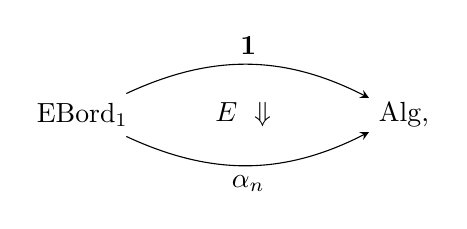
\begin{tikzpicture}[baseline=(current bounding box.center), >=stealth, scale=0.95]
  \node (A) at (0,0) {$\EBord_1$};
  \node (C) at (4.3,0) {$\Alg$,};
  \draw[->] (A) to[bend left=26] node[above] {$\mathbf 1$} (C);
  \draw[->] (A) to[bend right=26] node[below] {$\alpha_n$} (C);
  \node at (2.15,0) {$E\ \Downarrow$};
\end{tikzpicture}
\quad
\begin{array}{l@{\hspace{0.9em}}l}
E(\mathrm{pt}^{+})={}_{A}V, & E(\mathrm{pt}^{-})={}_{\ol{A}}\ol{V},\\[1pt]
E(\mathrm{I}^{+}_t)={}_{A}V\to{}_{A}V, & E(\mathrm{I}^{-}_t)={}_{\ol{A}}\ol{V}\to_{\ol{A}}\ol{V}\\[1pt]
E(\cap^{+}_t)=V\otimes_{\ol{A}}\ol{V}\to\C, & E(\cap^{-}_t)=\ol{V}\otimes_{A}V\to\C\\[1pt]
E(\cup^{+}_t)=\C\to V\otimes_{\ol{A}}\ol{V}, & E(\cup^{+}_t)=\C\to\ol{V}\otimes_{A}V\\[1pt]
E(S_t)\in V\otimes_{A\otimes\ol{A}}\ol{V} &
\end{array}
\end{array}
\tag{20}
\end{equation}
决定。翻译回定义 2.1，这引入 $\cH$ 上的一个 $A$-作用，并要求哈密顿量 $H$ 是 $A$-线性的。
% [Tutor Note: (20) 的 2-胞图中扭标作 $\alpha_n$，但本节由 (19) 定义的扭是 $\alpha_A$；(20) 正文又写 $\alpha_A$-扭场论，故图中 $\alpha_n$ 应读作 $\alpha_A$。原文如此，照排，已登记 ERRATA。]
% [Tutor Note: (20) 第四行第二个同样原写作 $E(\cup^{+}_t)$，按对称性应为 $E(\cup^{-}_t)$（与 (19) 的笔误同型）；照原样排，已登记 ERRATA。]
\end{example}

\begin{remark}[2.23]
与哈密顿量 $H$ 交换的算子是量子理论的\emph{对称性}。因此，上一个例子中 $A$-扭场论的例子也可以看作代数 $A$ 通过对称性作用的那些理论。
\end{remark}

\begin{example}[2.24（Spin 理论）]
为处理费米子（如例 2.11 那样），把配边范畴 $\EBord_1$ 加强为 $\EBord^{\mathrm{Spin}}_1$，其配边现在是带 spin 结构的欧几里得 1 维流形。spin 场论的目标范畴相应地把 $\Alg$ 加强为由 $\Z/2$-分次代数、$\Z/2$-分次双模以及保分次的双模映射构成的、带 $\Z/2$-分次张量积的双范畴。Spin 1 维流形有来自 spin 翻转的 $\Z/2$-自同构；类似地，$\Z/2$-分次代数与双模有来自其分次对合 $(-1)^{F}$ 的 $\Z/2$-自同构；见下文 (22)。更形式地说，$\EBord^{\mathrm{Spin}}_1$ 与 $\Alg$ 带有典范的 $B\Z/2$-作用。spin 场论于是是如 (11) 那样的反射正、$B\Z/2$-等变函子，而扭 spin 理论是相对于如 (20) 那样的 $B\Z/2$-等变函子的 $B\Z/2$-等变自然变换。这种 $B\Z/2$-等变性是 spin 统计定理的一个版本 [HST10, Definition 6]。

例 2.11 的自由费米子提供一个重要的例子：一个扭 spin 场论，其中 (19) 中的 $A=\mathrm{Cl}_n$ 定义扭，而 $E(\mathrm{pt}^{+})=V$ 作为 $\mathrm{Cl}_n$-模定义扭 spin 理论。半群是恒等，因此 1 维自由费米子确定一个\emph{拓扑的}扭 spin 理论。按照上一个注，$\mathrm{Cl}_n$-作用是保持作用量泛函 (9) 的经典平移对称性的量子化。要在配边框架中以正确的符号纳入这些对称性，就必须使用 spin 场论的形式体系。
% [Tutor Note: 原文此句写作 "a twisted spin field theory theory"，"theory" 重复一次；译文按单次处理，已登记 ERRATA。]
\end{example}
% [Tutor Note: 例 2.24 引用“下文 (22)”指的是 §3 中的式 (22)（$(-1)^{F}$ 的分次对合在该处正式出现），不属本块，属 sec3.tex。]


\clearpage
\section{超对称量子力学与 K 理论}
% sec3.tex — c03｜原文 p13（§3 标题下的正文起）–p19，并含 p20 上半至 §4 标题前
% §3 超对称量子力学与 K 理论（§3.1–§3.6）；本块公式号 (21)–(38)，共 18 条；编号环境 3.1–3.26
% 块边界：式 (20) 在 p13 顶部、§3 标题之上的 §2 例 2.22 内，不属本块。
% 图 3（p15 顶部）、图 4（p18 顶部）一律从略，用 \figomit。
% [Tutor Note: 底本 p13 页首的式 (20) 排在 §3 标题之前，属 §2 例 2.22 中 A-扭场论的数据；故本节从式 (21) 起，式 (20) 见第 2 节末。]
% [Tutor Note: 注 3.25 末句与例 3.26 排在 p20 页首、§4 标题之前，编号仍属 §3，故本块译至 §4 标题前止；这是底本的分页所致，非编号错乱。]

% [原文 p.13]
本节的目标是解释猜想 1.1 的下述类比。

\begin{conjecture}[3.1（Stolz–Teichner）]
对每个 $n\in\Z$，存在虚线箭头
\begin{equation}
\begin{tikzpicture}[baseline=(current bounding box.center), >=stealth]
  \node (A) at (0,3.4) {$\left\{\begin{array}{c}\text{一族 $n$ 维 spin$^c$}\\[2pt] \text{流形 $M\to X$}\end{array}\right\}$};
  \node (C) at (9.4,1.7) {$\mathrm{K}^{-n}(X)$};
  \node (B) at (0,0) {$\left\{\begin{array}{c}\text{$X$ 上次数为 $-n$ 的}\\[2pt] \text{1 维超对称}\\[2pt] \text{场论}\end{array}\right\}$};
  \draw[->] (A.south east) -- node[above, sloped] {拓扑指标} (C.north west);
  \draw[->, dashed] (A.south) -- node[left] {量子化} (B.north);
  \draw[->, dashed] (B.east) -- node[below right=1pt, pos=0.42] {上闭链${}_{-n}$} (C.south west);
\end{tikzpicture}
\tag{21}
\end{equation}
使三角形交换；其中“拓扑指标”是 Atiyah–Bott–Shapiro 的 spin$^c$ 定向 [ABS64]，“量子化”是对 $M$ 上超对称力学的量子化，“上闭链$_n$”把 $X$ 上的一个量子理论送到 $\mathrm{K}^n(X)$ 中的一个类。当 $n$ 为负时，空流形是唯一的 spin 流形，此时 (21) 的内容是存在一个上闭链映射。
\end{conjecture}
% [Tutor Note: 猜想 3.1 的流形是 spin^c 流形（式 (21) 图中为 spin^c），而正文此处说 "the only spin manifold"；照译，应读作 spin^c 流形。]
% [Tutor Note: 式 (21) 的箭头标签是 cocycle_{−n}，紧邻正文却写 cocycle_n；与式 (1) 同一情形，下标随度数变号，二者不矛盾。]

除某些技术性告诫外，猜想 3.1 是一个定理。事实上，它已对 [ST04, §3.2] 与 [HST10] 中 1 维超对称场论的定义得到验证，其综述见 §3.3 与下文假设 3.20。然而，人们相信这些既有论证难以很好地推广到 $2|1$ 维情形，因此猜想 3.1 的各种变体仍然悬而未决；其中一个变体见注 3.24。

% [原文 p.14]
\subsection{超对称量子力学的动机}
给定定义 2.1 意义下的一个量子力学系统 $(\cH,H)$，设 $\cH=\cH^+\oplus\cH^-$ 带有一个 $\Z/2$-分次，且 $H$ 尊重该分次（即 $H$ 是偶映射）。等价地，$\cH$ 上带有一个对合 $(-1)^F\colon\cH\to\cH$，其特征子空间为
\begin{equation}
(-1)^F=\begin{cases}+1 & \text{在 } \cH^+ \text{ 上}\\ -1 & \text{在 } \cH^- \text{ 上}\end{cases}
\qquad\text{且}\qquad H(-1)^F=(-1)^F H.
\tag{22}
\end{equation}
超对称量子力学在这些数据之上增添 $\cN$ 个奇算子 $Q_i$，满足
\begin{equation}
Q_i^2=H,\quad [Q_i,Q_j]=Q_iQ_j+Q_jQ_i=0\ (i\ne j),\quad [(-1)^F,Q_i]=0,\quad i\in\{1,2,\dots,\cN\}
\tag{23}
\end{equation}
其中 $[-,-]$ 是分次交换子 [Wit82a, §2]。$Q_i$ 是超对称算子。

\begin{example}[3.2（定向流形上的 $\cN=2$ 超对称量子力学）]
超对称量子力学的经典例子取状态空间为 $\cH=\Omega^\bullet(M)$，即定向 Riemann 流形 $M$ 上的微分形式 [Wit82b, §2]。此时哈密顿量定义为 Hodge 拉普拉斯算子 $H=\dd\dd^*+\dd^*\dd$，它有一对交换的奇平方根
\begin{equation}
Q_1=\dd+\dd^*,\qquad Q_2=\sqrt{-1}(\dd-\dd^*),\qquad [Q_1,Q_2]=0,\qquad Q_1^2=Q_2^2=H.
\tag{24}
\end{equation}
这是 $\cN=2$ 超对称的数据。忘掉 (24) 中一个 $Q_i$ 便抽取出一个 $\cN=1$ 理论。其他 $\cN=1$ 理论来自（扭的）Dirac 算子，见例 3.13。
\end{example}

猜想 3.1（以及下文）的焦点是 $\cN=1$ 超对称。此时，(23) 中的算子确定超 Lie 群 $\R^{1|1}$ 的超 Lie 代数的一个表示，$\R^{1|1}$ 的乘法为\footnote{这个公式应在 $\R^{1|1}$ 的函子点（functor of points）意义下理解，例如参见 [DM99]。}
\begin{equation}
(t,\theta)\cdot(s,\eta)=(t+s+\theta\eta,\theta+\eta),\qquad (t,\theta),(s,\eta)\in\R^{1|1}.
\tag{25}
\end{equation}
沿 $\theta=0$ 包含，得到通常加法下的 Abel 子群 $\R<\R^{1|1}$。沿此包含作延拓，就把通常的时间演化 (6) 推广为半超群（supersemigroup）的一个表示 [HST10, §5] [ST04, §3.2]
\begin{equation}
\R^{1|1}_{\ge0}\to\mathrm{End}(\cH),\qquad (t,\theta)\mapsto\ee^{-tH+\theta Q},
\tag{26}
\end{equation}
其中 $(t,\theta)$ 是子超流形 $\R^{1|1}_{\ge0}\subset\R^{1|1}$（$t\ge0$）上的坐标。
% [Tutor Note: p14 的两条脚注在原文中为第 5 号（$\R^{1|1}$ 的函子点，见上）与第 6 号（奇无界算子的定义域，见 §3.2）；译本由 LaTeX 自动编号，号码不必相同。]

\begin{definition}[3.3]
具有（$\cN=1$）超对称的一个量子力学系统是一对 $(\cH,Q)$，其中 $Q$ 是 Hilbert 空间 $\cH$ 上的奇无界自伴算子，它生成一个迹类（trace class）的超半群表示 (26)。若存在酉映射 $u\colon\cH\to\cH'$ 使 $Q'=uQu^{-1}$，则称系统 $(\cH,Q)$ 与 $(\cH',Q')$ 等价。
\end{definition}

我们在下文展开这一点。

\subsection{具有 $\cN=1$ 超对称的次数为 $n$ 的量子系统的空间}
与 §2.1 中描述的哈密顿量空间类似，我们把定义 3.3 推广为带超对称的量子系统的空间——并最终推广为一个栈。着眼 K 理论上的 $\Z$-分次，我们还纳入 Clifford 模结构；在物理上，这些结构来自自由费米子的（射影）对称性代数，见例 2.11 与注 2.23。

固定一个无穷维可分 $\Z/2$-分次 Hilbert 空间 $\cH$，其偶子空间与奇子空间都是无穷维的。置 $\cH_n:=\mathrm{Cl}_n\otimes\cH$，其中 $\mathrm{Cl}_n$ 是第 $n$ 个 Clifford 代数。设 $Q$ 是 $\cH_n$ 上的 Clifford 线性奇自伴无界算子。\footnote{$\Z/2$-分次 Hilbert 空间上的奇无界算子，其定义域 $\mathrm{dom}(Q)\subset\cH$ 是分次子空间，且 $Q\colon\mathrm{dom}(Q)\to\cH$ 是奇线性映射。} 注意 $H=Q^2$ 是 Clifford 线性的、非负的偶算子。对 $H=Q^2$ 应用谱定理，得到一族互相正交的特征子空间 $\{\cH_\lambda\subset\cH_n\}_{\lambda\ge0\in\R}$，如
% [原文 p.15]
图 1 所示。\figomit{3}{推广图 1：超对称把标号 $\cH_\lambda\subset\cH$ 增强为一个 $\Z/2$-分次以及一个满足 $Q_\lambda^2=\lambda\cdot1$（$\lambda\ge0$）的奇算子 $Q_\lambda$。沿用 [Wit82a]，我们用一个 $\circ$ 记一维偶空间、用一个 $\times$ 记一维奇空间（分别代表玻色态与费米态）。由于 $\lambda\ne0$ 时 $Q_\lambda$ 可逆，$\cH_\lambda$（$\lambda\ne0$）上的偶维数必须等于奇维数。因此，零特征子空间中偶维数与奇维数之差是形变不变量 $[\cH_0]\in\mathrm{K}(\mathrm{pt})$。}
这些子空间是有限秩 $\Z/2$-分次 $\mathrm{Cl}_n$-模，带有奇算子 $Q_\lambda$ 的作用，其特征值为 $\pm\sqrt{\lambda}$。当 $\lambda\ne0$ 时，算子 $\frac{1}{\sqrt{\lambda}}Q$ 在 $\cH_\lambda$ 上生成一个与 $\mathrm{Cl}_n$-作用交换的 $\mathrm{Cl}_{-1}$-作用。因此，$\lambda\ne0$ 时的 $\cH_\lambda$ 获得 $\mathrm{Cl}_{-1}\otimes\mathrm{Cl}_n$-模的结构。于是这些构形的形变（例如见图 3）重新得到 Atiyah–Bott–Shapiro 对 $\pi_*\mathrm{K}^n$ 的系数的描述：$\mathrm{Cl}_n$-模的同构类模掉那些可延拓为 $\mathrm{Cl}_{-1}\otimes\mathrm{Cl}_n$-模者 [ABS64]。
% [Tutor Note: 原文把指标集写作 $\{\cH_\lambda\subset\cH_n\}_{\lambda\ge0\in\R}$；照排，应读作 $\lambda\in\R_{\ge0}$。]
% [Tutor Note: 图 3 图注中的 "o's" 指图上小圆圈 $\circ$；本译作「一个 $\circ$ 记一维偶空间」，与图中记号一致。]

\begin{definition}[3.4]
记 $\sHam^n$ 为生成迹类超半群表示 (26) 的奇自伴 $\mathrm{Cl}_n$-线性无界算子 $Q$ 构成的空间。
\end{definition}

\begin{remark}[3.5]
无界算子 $Q$ 何时确定一个迹类超半群表示，其分析条件见 [HST10, §5]。
\end{remark}
% [Tutor Note: 定义 3.4 与定义 3.7 在原文中用上标 $\sHam^n$、$\SQM^n$，而命题 3.12 的证明与式 (31) 等处用下标；照原文混用，不改。]

\begin{definition}[3.6]
对 $\Z/2$-分次 Hilbert 空间，定义（超）酉群
\[
\mathrm{U}^\pm(\cH)\simeq\left\{u\in\mathrm{U}(\cH)\ \middle|\ u=\begin{bmatrix}*&0\\0&*\end{bmatrix}\ \text{或}\ \begin{bmatrix}0&*\\*&0\end{bmatrix}\right\}
\]
其中 $u$ 相对分解 $\cH=\cH^+\oplus\cH^-$（偶子空间与奇子空间）取分块形式。群 $\mathrm{U}^\pm(\cH)$ 是分次的（例如在 [Fre12] 的意义下），分次由同态
\[
\mathrm{U}^\pm(\cH)\to\pi_0(\mathrm{U}^\pm(\cH))\simeq\Z/2
\]
给出，后者读出酉映射保持还是反转 $\cH$ 上的分次。记 $\mathrm{PU}^\pm(\cH):=\mathrm{U}^\pm(\cH)/\mathrm{U}(1)$ 为射影化。类似地，对分次酉 $\mathrm{Cl}_n$-模 $\cH_n$，定义 $\mathrm{U}^\pm(\cH_n)$ 为与 Clifford 作用交换的酉变换，并记 $\mathrm{PU}^\pm(\cH_n)=\mathrm{U}^\pm(\cH_n)/\mathrm{U}(1)$ 为射影化。
\end{definition}

\begin{definition}[3.7]
定义拓扑群胚 $\SQM^n:=\sHam^n/\!/\mathrm{PU}^\pm(\cH_n)$ 为酉群的共轭作用所诱导出的作用的商。
\end{definition}

我们有定义 2.8 的下述超对称推广。

\begin{definition}[3.8]
设 $G$ 是紧 Lie 群。带 $G$-对称性的次数 $n$ 的超对称量子力学系统构成的栈，是映射栈 $\mathrm{Map}(\mathrm{pt}/\!/G,\SQM^n)$。
\end{definition}
展开之，$\mathrm{Map}(\mathrm{pt}/\!/G,\SQM^n)$ 中的一个点是同态 $\alpha\colon G\to\mathrm{PU}^\pm(\cH)$，它定义 $G$ 的一个中心扩张 $G^\alpha$ 以及一个酉表示 $G^\alpha\to\mathrm{U}^\pm(\cH)$（类似于 (8)），连同 $\cH$ 上与 $G^\alpha$-作用交换的一个超对称生成元 $Q$。复合 $G^\alpha\to\mathrm{U}^\pm(\cH)\to\Z/2$ 赋予群 $G^\alpha$ 一个分次，它读出哪些元素以保分次或反分次的自同构作用在 $\cH$ 上。

% [原文 p.16]
\subsection{超对称量子力学与 K 理论}
Atiyah–Bott–Shapiro 对分次环 $\pi_{-*}\mathrm{K}=\mathrm{K}^*(\mathrm{pt})$ 的描述 [ABS64] 给出一个映射
\begin{equation}
\sHam^n\to\mathrm{K}^n(\mathrm{pt}),\qquad Q\mapsto[\mathrm{Index}(Q)]:=[\mathrm{Ker}(Q)]=[\cH_0]
\tag{27}
\end{equation}
它把超对称生成元 $Q$ 送到其核，视作一个有限秩 $\mathrm{Cl}_n$-模。

\begin{definition}[3.9]
$Q\in\sHam^n$ 的 Witten 指标是它在 (27) 下的像。
\end{definition}

事实上，我们得到下述结论。

\begin{theorem}[{3.10（[HST10]，[Che08]）}]
空间 $\sHam^n$ 表示函子 $\mathrm{K}^n(-)$。
\end{theorem}
\begin{proof}[证明梗概]
空间 $\sHam^n$ 同伦等价于一个 Clifford 线性 Fredholm 算子空间，后者已知表示 K 理论谱中的第 $n$ 个空间 [AS69]。事实上，$Q\in\sHam^n$ 中算子特征值的增长条件保证：由泛函演算定义的算子 $Q/(1+Q^2)$ 是 Fredholm 的。
\end{proof}

\begin{example}[3.11（拓扑理论）]
推广例 2.5：任何有限维 $\Z/2$-分次子模 $V\subset\cH_n$ 都通过取 $Q=0$、定义域为 $V$ 而确定 $\sHam^n$ 中的一个点。这对应于支撑在 $0\in\R_{\ge0}$、标号为 $\cH_0=V$ 的构形。我们注意到，自然包含
\begin{equation}
\left\{\begin{array}{c}\text{次数 $n$}\\[2pt]\text{拓扑理论}\end{array}\right\}\xrightarrow{\ \text{群完备化}\ }\sHam^n\to\SQM^n
\tag{28}
\end{equation}
可以与 $\mathrm{Cl}_n$-模的群完备化等同起来。
\end{example}

\begin{proposition}[3.12]
$\{\SQM^n\}_{n\in\Z}$ 表示拓扑栈的扭 K 理论，特别地表示紧 Lie 群 $G$ 的 $G$-空间上的扭等变 K 理论 [FHT11a]。
\end{proposition}
\begin{proof}[证明略述]
给定拓扑栈的一个映射 $\alpha$，
\begin{equation}
\mathfrak X\xrightarrow{\ \alpha\ }\SQM^n=\sHam^n/\!/\mathrm{PU}^\pm(\cH_n)
\tag{29}
\end{equation}
与投影作后复合，便确定一个映射 $\tau\colon\mathfrak X\to\mathrm{pt}/\!/\mathrm{PU}^\pm(\cH_n)$，它分类一个带 Clifford 作用的射影 Hilbert 丛 $\PP\cH^\tau\to\mathfrak X$（也称为扭 Hilbert 丛 [FHT11a, §3.2]）。此外，该丛由分次 gerbe $\mathrm{pt}/\!/\mathrm{U}^\pm(\cH_n)\to\mathrm{pt}/\!/\mathrm{PU}^\pm(\cH_n)$ 沿 $\tau$ 的拉回来分类。映射 $\alpha$ 的其余数据，是 $\mathfrak X$ 上以 $\sHam_n$ 为纤维的配丛的一个截面。由于 $\sHam_n$ 表示 $\mathrm{K}^n(-)$，该截面的同伦类是一个扭 K 理论类。特殊化到（好的）空间 $X$ 在紧 Lie 群 $G$ 作用下的商栈 $\mathfrak X=X/\!/G$，便重新得到 $X$ 的 $G$-等变扭 K 理论 [FHT11a, §3.5.4]。
\end{proof}

\subsection{超对称量子力学与指标定理}

\begin{example}[3.13（spin$^c$ 流形上的超对称量子力学）]
设 $M$ 是 Riemann 流形，考虑路径 $x\colon\R\to M$ 连同（费米子）$\psi\in\Gamma(\R;x^*TM)$ 的经典理论，其作用量为
\begin{equation}
S(x,\psi)=\frac12\int_\R(\|\dot x\|+\langle\psi,\nabla_{\dot x}\psi\rangle)\dd t.
\tag{30}
\end{equation}
设 $M$ 带有一个选定的 spin$^c$ 结构，其旋量丛 $\mathrm{S}:=P\times_{\mathrm{Spin}(n)}\mathrm{Cl}_n$ 支撑 $\mathrm{Cl}_{-n}$-线性的 Dirac 算子 $\mathord{\not{D}}$。\footnote{右 $\mathrm{Cl}_n$-模之丛 $\mathrm{S}=P\times_{\mathrm{Spin}(n)}\mathrm{Cl}_n$ 确定一个左 $\mathrm{Cl}_{-n}=\mathrm{Cl}^{op}_n$-模之丛。} 那么经典理论 (30) 量子化后状态空间为 $\cH=\Gamma(\mathrm{S})$、哈密顿量为 $H=\mathord{\not{D}}^2$ [Fre99, 第 43–44 页]。取 $Q=\mathord{\not{D}}$ 便按定义 3.7 的意义定义一个次数为 $-n$ 的超对称量子系统，从而给出
\begin{equation}
\left\{\begin{array}{c}\text{$n$ 维 spin$^c$}\\[2pt]\text{流形 $M$}\end{array}\right\}\to\SQM_{-n},\qquad M\mapsto\mathord{\not{D}}.
\tag{31}
\end{equation}
若 $M$ 带保持 spin$^c$ 结构的 $G$-作用，则 $\Gamma(\mathrm{S})$ 自然地是 $G$-表示。若改为 $W_3(TM)\in\mathrm{H}^3_G(M;\Z)$ 从 $BG$ 的上同调（即点的等变上同调）拉回，则 $\Gamma(\mathrm{S})$ 只有射影的 $G$-作用。两种情形都给出定义 3.8 意义下带 $G$-对称性的超对称量子力学系统。
\end{example}
% [Tutor Note: 式 (30) 的动能项原文作 $\|\dot x\|$（未平方）；通常写作 $\|\dot x\|^2$。照原文排，疑为笔误，已登记 ERRATA。]
% [Tutor Note: p16 的脚注为原文第 7 号（右 $\mathrm{Cl}_n$-模丛与左 $\mathrm{Cl}_{-n}$-模丛的对应），译本自动编号。]

% [原文 p.17]
\begin{proof}[猜想 3.1 的证明梗概]
若把 $X$ 上次数为 $-n$ 的 1 维超对称欧几里得场论定义为映射 $X\to\Ham(\cH_{-n})$（比较 [ST04, Definition 3.2.10]），则 (21) 中的上闭链映射由命题 3.12 得出。给定 spin$^c$ 流形的一族 $M\to X$，逐纤维的 $\mathrm{Cl}_{-n}$-线性 Dirac 算子给出 (31) 的族版本，从而产生一个映射 $X\to\Ham(\cH_{-n})$，它对应于族解析指标 [ST04, Remark 3.2.21]。三角形 (21) 的交换性就是族指标定理 [AS71]。
\end{proof}

\begin{remark}[3.14]
指标定理的物理论证考察 $M$ 上超对称量子力学的时间演化半群的极限
\begin{equation}
\mathrm{sTr}_{\mathrm{Cl}_{-n}}\bigl(\ee^{-t\mathord{\not{D}}^2}\bigr)=\begin{cases}\mathrm{Index}(\mathord{\not{D}}) & t\to\infty\\[6pt] \displaystyle\int_X\hat{A}(X) & t\to0.\end{cases}
\tag{32}
\end{equation}
McKean–Singer 定理 [MS67] 表明该超迹不依赖于 $t$，并把 $t\to\infty$ 极限与 $Q=\mathord{\not{D}}$ 的（Witten）指标等同起来。另一方面，$t\to0$ 极限可用路径积分技巧计算。具体地，超对称局部化把该路径积分等同于 $\hat{A}$-形式在 $M$ 上的积分 [Wit82b, AG83]。数学处理参见 [Ati85, JP90, BGV92]。
\end{remark}

K 理论中的拓扑前推来自 Thom 同构，后者也有一个用超对称量子力学的描述。

\begin{example}[3.15（自由费米子的超对称形变）]
由例 3.11，例 2.11 与 2.24 中的自由费米子有到次数 $n$ 超对称理论的一个典范延拓：状态空间是分次 $\mathrm{Cl}_n$-模 $V$，超对称生成元为 $Q=0$。考虑修改后的自由费米子经典场论 (9)
\begin{equation}
\psi\colon\R\to\R^n,\qquad S(\psi)=\frac12\int_\R(\langle\psi,\partial_t\psi\rangle+\langle x,\psi\rangle)\dd t
\tag{33}
\end{equation}
它把源项 $\langle x,\psi\rangle$ 加到作用量上，其中 $x\in\R^n$ 固定。该系统的量子化给出状态空间 $V=\mathrm{Cl}_n$（作为左 $\mathrm{Cl}_n$-模），连同由超对称生成元 $Q=\mathrm{cl}_x\colon V\to V$ 决定的时间演化算子，其中 $\mathrm{cl}_x$ 是沿 $x\in\Pi\R^n\subset\mathrm{Cl}_n$ 的右 Clifford 乘法。让 $x\in\R^n$ 变动，得到映射
\begin{equation}
\R^n\to\SQM^n,\qquad x\mapsto Q=\mathrm{cl}_x
\tag{34}
\end{equation}
它在 $x=0$ 处是拓扑理论。可以把 (34) 与 K 理论中第 $n$ 个悬置类等同起来 [ABS64]。存在 (33) 上的 $\mathrm{O}_n$-作用，它旋转 $\psi$ 与源项 $x$，而映射 (34) 是（射影地）$\mathrm{O}_n$-等变的。这给出 (10) 的推广
\begin{equation}
\Th_n\colon\R^n/\!/\mathrm{O}_n\to\SQM^n=\sHam^n/\!/\mathrm{PU}^\pm(\cH),\qquad
\begin{gathered}\mathrm{O}_n\to\mathrm{PU}^\pm(\cH),\\ x\mapsto\mathrm{cl}_x=Q(x),\quad x\in\R^n\end{gathered}
\tag{35}
\end{equation}
其中映射 $\mathrm{O}_n\to\mathrm{PU}^\pm(\cH_n)$ 分类 $\mathrm{Pin}^c$-扩张。在命题 3.12 之下，(35) 底层的扭 K 理论类是第 $n$ 个泛（扭等变）Thom 类 $[\Th_n]\in\mathrm{K}^{w_1+W_3}(\R^n/\!/\mathrm{O}_n)_c\simeq\mathrm{K}^{w_1+W_3}_{\mathrm{O}_n}(\R^n)_c$ [FHT11a, §3.6] [ST04, Remark 3.2.22]。
\end{example}
% [Tutor Note: 式 (35) 中写 $\mathrm{PU}^\pm(\cH)$，紧接正文写 $\mathrm{PU}^\pm(\cH_n)$；原文如此，照排。]
% [Tutor Note: Thom 类的次数写作 $w_1+W_3$（小写 $w_1$、大写 $W_3$）；通常记作 $w_1+w_3$，$W_3$ 是 spin^c 结构的整提升。照原文排。]

\begin{remark}[3.16]
Mathai–Quillen 形式化 [MQ86] 计算 (33) 的配分函数，重新得到由 $\mathfrak{o}_n$ 上（逆）$\hat{A}$-形式所决定的一个泛 Thom 类。
\end{remark}
% [Tutor Note: 上句原文末为 "on o_n"，其中 o_n 是 Fraktur 体 $\mathfrak{o}_n$（$\mathrm{O}_n$ 的 Lie 代数），文字层易误读作 "on on"。]

\subsection{配边框架中的超对称量子力学}
可以把超对称量子力学重新打包成 $1|1$-欧几里得配边范畴 $\EBord_{1|1}$ 的一个表示，它推广 $\EBord_1$。$\EBord_{1|1}$ 的对象是 $\bullet=\mathrm{spt}^+$ 与 $\circ=\mathrm{spt}^-$ 的有限不交并，即带两种定向选取的超点。态射见图 4，其中 $(t,\theta)\in\R^{1|1}_{\ge0}$ 编码一个“超长度”。与之前类似，我们得到与配边复合相关联的关系，例如
\begin{equation}
\mathrm{I}^\pm_{s,\eta}\circ\mathrm{I}^\pm_{t,\theta}\simeq\mathrm{I}^\pm_{s+t\pm\eta\theta,\eta+\theta},
\tag{36}
\end{equation}
它们给出 (26) 中超半群 $\R^{1|1}_{\ge0}$ 中乘法的几何对应物。

\figomit{4}{$\EBord_{1|1}$ 中的态射是上述生成元的有限不交并。它们把图 2 中的生成元加以增强：加入 spin 结构，并把长度参数 $t\in\R_{\ge0}$ 换成取值于 $\R^{1|1}_{\ge0}$ 的“超长度”$(t,\theta)$。}

% [原文 p.18]
\begin{remark}[3.17]
维数为 $1|1$ 的超欧几里得几何由超 Lie 群 (25) 按如下意义决定：人们规定群 $\R^{1|1}$ 以欧几里得等距的方式作用在超流形 $\R^{1|1}$ 上。这类似于维数为 $1$ 的欧几里得几何由下述规定决定：群 $\R$ 是 $\R$ 的保向对称群，通过平移作用。此外还有一个由 $\theta\mapsto-\theta$ 确定的 $1|1$-欧几里得等距，起 spin 翻转的作用。因此，$1|1$-欧几里得场论推广了例 2.24 中的 spin 欧几里得场论。下文我们隐式地施加相应的 $B\Z/2$-等变性质，细节参见 [ST11, §4.3]。
\end{remark}

沿用 (19)，我们对每个 Clifford 代数 $\mathrm{Cl}_n$ 构造一个扭。

\begin{definition}[3.18（次数扭）]
次数扭由下述指派决定：
\begin{align}
&\alpha_n\colon\EBord_{1|1}\to\Alg,\notag\\
&\alpha_n(\mathrm{spt}^+)=\mathrm{Cl}_n,\quad \alpha_n(\mathrm{spt}^-)=\mathrm{Cl}^{op}_n=\mathrm{Cl}_{-n},\notag\\
&\alpha_n(\mathrm{I}^\pm_{t,\theta})={}_{\mathrm{Cl}_n}(\mathrm{Cl}_n)_{\mathrm{Cl}_n},\quad
 \alpha_n(\cap^+_{t,\theta})=(\mathrm{Cl}_n)_{\mathrm{Cl}_n\otimes\mathrm{Cl}^{op}_n},\notag\\
&\alpha_n(S^\pm_{t,\theta})=\mathrm{Cl}_n\otimes_{\mathrm{Cl}_n\otimes\mathrm{Cl}^{op}_n}\mathrm{Cl}_n,\notag\\
&\alpha_n(\cup^+_{t,\theta})={}_{\mathrm{Cl}_n\otimes\mathrm{Cl}^{op}_n}\mathrm{Cl}_n,\tag{37}
\end{align}
其反射结构来自 Clifford 代数上的 $\ast$-结构 $\ast\colon\mathrm{Cl}_n\xrightarrow{\sim}\ol{\mathrm{Cl}^{op}_n}=\ol{\mathrm{Cl}}_{-n}$。这些值与 $(t,\theta)$ 无关，因此次数扭是拓扑的。次数 $n$ 的扭场论的取值可以类比 (20) 读出。Morita 等价 $\mathrm{Cl}_n\otimes\mathrm{Cl}_m\simeq\mathrm{Cl}_{n+m}$ 给出扭的同构 $\alpha_n\otimes\alpha_m\simeq\alpha_{n+m}$（$n,m\in\Z$）。
\end{definition}
% [Tutor Note: 式 (37) 的 ${}_{\mathrm{Cl}_n}(\mathrm{Cl}_n)_{\mathrm{Cl}_n}$ 是双模记号：左作用写在左、右作用写在右；$\mathrm{Cl}^{op}_n=\mathrm{Cl}_{-n}$ 由 Clifford 代数的 $8$ 周期性与取反代数给出。]
% [Tutor Note: 式 (37) 中 $\otimes_{\mathrm{Cl}_n\otimes\mathrm{Cl}^{op}_n}$ 是平衡张量积（coequalizer），不是分次张量积。]

\begin{remark}[3.19]
Clifford 代数都是 2-范畴 $\Alg$ 中的可逆对象，因此是全对偶的（fully dualizable）。由配边假设 [Lur09a]，$\mathrm{Cl}_n$ 确定一个全扩张的 2 维拓扑场论。该理论在 $0$ 维与 $1$ 维流形上的取值由 (37) 给出 [Gun16]。因此，次数扭是这个全扩张拓扑场论的一个截断，其反射结构继承自 $\mathrm{Cl}_n$ 上的 $\ast$-结构。
\end{remark}
% [Tutor Note: 原文 "with reflection structure inherited the ∗-structure" 缺介词 from，应为 inherited from；中文译文已按正确意思作「继承自」，已登记 ERRATA。]

令 $\QFT^\alpha_{1|1}(\mathfrak X)$ 记 $\mathfrak X$ 上 $\alpha$-扭的反射正 $1|1$ 维欧几里得场论的群胚（见定义 1.9）。反射正性与定义 2.13 中的基本相同。我们先分析次数扭 (37) 对应的群胚 $\QFT^n_{1|1}:=\QFT^{\alpha_n}_{1|1}(\mathrm{pt})$。

\begin{hypothesis}[{3.20（比较 [ST04, Proposition 3.2.6] 与 [HST10, Corollary 6.38]）}]
存在栈的满射（epimorphism）$\QFT^n_{1|1}\to\SQM^n$。
\end{hypothesis}
\begin{proof}[略证]
论证与假设 2.14 的论证类似，因此我们将（更加）简略。函子 $\QFT^n_{1|1}\to\SQM^n$ 把 $1|1$-欧几里得场论 $E$ 送到其半超群表示 $E(\mathrm{I}^+_{t,\theta})$ 的生成元 $Q$。确实，由 [HST10, Lemma 5.10]，有 $E(\mathrm{I}^+_{t,\theta})=\ee^{-tH+\theta Q}$，其中 $Q$ 是由此唯一确定的无界奇 Clifford 线性算子，定义域为 $E(\mathrm{spt}^+)\subset\cH$。

为说明该指派确定一个满射，$\EBord_{1|1}$ 的生成元与关系表示（比较 [HST10, Theorem 6.42]）表明：次数 $n$ 的 $1|1$-欧几里得场论由自伴 Clifford 模 $\bigl(E(\mathrm{spt}^+),\langle-,-\rangle\bigr)$ 以及来自 $E(\mathrm{I}^+_{t,\theta})$ 的自伴 $\mathrm{Cl}_n$-线性半超群表示决定。类比于 (11) 的构造随后确定所要的单侧逆函子。
\end{proof}

% [原文 p.19]
\begin{remark}[3.21]
对栈的等价 $\QFT^n_{1|1}\to\SQM^n$ 的期望会遇到一个障碍：存在许多互不同构的拓扑向量空间 $E(\mathrm{pt}^+)$，它们导致互不同构的场论，但这些场论在 $\SQM^n$ 中作为对象却是同构的（在把一个拓扑内积空间完备化为 Hilbert 空间之后）。一种可能的修补是施加一个更弱的等价关系。场论的 concordance 类 [ST11, Definition 1.12] 是最有希望的选择，并且人们期望：$X$ 上场论的 concordance 类与从 $X$ 到栈 $\QFT^n_{1|1}$ 的映射的 concordance 类一一对应。然而，concordance 等价 $\QFT^n_{1|1}\to\SQM^n$ 仍要求对场论的定义作进一步的技术性修改，参见 [ST11, Remark 3.16] 与 [Ulr21]。粗略地说，必须允许其状态空间是秩非常数的向量丛的场论族，其中秩的变化模仿一族 Dirac 算子的指标丛的跳跃。
\end{remark}

\subsection{来自配边框架的额外洞见}
延展 §2.3 中的想法，配边框架对带超对称的量子力学系统提供如下修饰。

\begin{example}[3.22（定向反转、KO 与 KR）]
仿照例 2.17，$\EBord_{1|1}(\mathfrak X)$ 上的定向反转通过前复合给出 $\mathfrak X$ 上（扭）场论群胚的一个 $\Z/2$-作用。取（同伦）不动点，得到无定向的 $1|1$ 维欧几里得场论（见 [HST10, Example 6.16]）。$\Z/2$-不动数据仍是状态空间上的一个实结构 (15)，并且要求时间演化算子是实的。因此，无定向理论对应于 $\KO$ 理论，见 [HST10, §6.8]。一个进一步的变体（与 Atiyah 的 $\KR$ 理论有关）以带 $\Z/2$-作用的栈 $\mathfrak X$ 为输入；这通过配边的定向反转与 $\mathfrak X$ 上的 $\Z/2$-作用两者确定 $\EBord_{1|1}(\mathfrak X)$ 上的一个 $\Z/2$-作用，进而给出场论上的 $\Z/2$-作用。
\end{example}

\begin{example}[3.23（带超联络的超向量丛）]
Dumitrescu [Dum12] 与 Stoffel [Sto19] 描述了例 2.20 与 2.21 到 $1|1$ 维欧几里得场论的推广。具体地，给定光滑流形 $X$ 上带 Quillen 超联络 $\mathbb{A}$ 的（有限秩）超向量丛 $V\to X$，Dumitrescu 构造了沿 $X$ 中 $1|1$ 维超路径的超平行移动。这给出一个函子
\begin{equation}
\mathrm{sPar}\colon\Vect^{\mathbb{A}}(X)\to\QFT^1_{1|1}(X).
\tag{38}
\end{equation}
对 $X$ 上的 gerbe $\alpha$，Stoffel 给出 (38) 的 $\alpha$-扭推广。
\end{example}

\begin{remark}[3.24]
(38) 的一个单侧逆取值于未必有限秩的向量丛上的超联络 [BE23b]。这在 [ST11] 的框架中证明了猜想 3.1 的一部分：Clifford 线性超联络的指标丛给出从场论到 K 理论所要的上闭链映射。对一族 spin$^c$ 流形，Bismut 的超联络 [Bis86] 进一步给出 (21) 中量子化映射的部分构造。要在此框架中完成猜想 3.1 的证明，只需对 Bismut 超联络构造 Dumitrescu 的超平行移动 (38) 的一个无穷秩推广，从而得到 (21) 中的“量子化”箭头。
\end{remark}
% [Tutor Note: 原文此处作 "it would suffice to to construct"，重复了 to；中文不受影响，已登记 ERRATA。]

\begin{remark}[3.25]
由于 $\EBord_{1|1}(\mathfrak X)$ 中的配边是超流形，所涉及的模空间可能很微妙，例如参见 [Wit19]。对 $\mathfrak X=\mathrm{pt}$ 上的场论，全部超几何本质上都被收纳进“超长度”参数 $(t,\theta)\in\R^{1|1}_{\ge0}$。然而，对栈 $\mathfrak X$ 上的配边，超的方面变得更加复杂。例如，对流形 $X$，$E\in\QFT^1_{1|1}(X)$ 在超圆上的取值确定一个微分形式 $Z_E\in C^\infty\bigl(\mathrm{Map}(\R^{0|1},X)\bigr)\simeq\Omega^\bullet(X)$，它与 (38) 结合起来可解释为场论族的 Chern 特征 [Han08]。更一般地，函数
% [原文 p.20]
在超栈 $\mathrm{Map}(\R^{0|1},X/\!/^{\nabla}G)$ 上给出等变 de Rham 上同调的一个模型 [Wu05, Sto13]，并引出 $1|1$-欧几里得场论的等变 Chern 特征 [BEH16]。若没有 [ST11] 的“超配边”框架，我们不知道有什么办法可以获得这些更精细的信息。
\end{remark}

\begin{example}[3.26（射影 $G$-表示）]
把超对称加到例 2.18 与 2.19 上，范畴 $\EBord_{1|1}(\mathrm{pt}/\!/^{\nabla}G)$ 把带联络的 $G$-丛加到图 4 所描绘的配边上。把超区间的半超群 $\mathrm{I}^+_{t,\theta}$ 限制到 $\theta=0$，得到一个与 (16) 所描绘的通常区间上的 $G$-丛等价的 $\EBord_{1|1}(\mathrm{pt}/\!/^{\nabla}G)$ 子范畴。因此，人们重新得到与之前相同的信息，但带有额外的增强。第一，超对称确定先前哈密顿量 $H$ 的一个平方根 $Q$。第二，超流形上 $G$-丛的联络更为复杂，涉及等变微分形式的几何。进一步讨论参见 [BEH16]。
\end{example}


\clearpage
\section{椭圆上同调与二维超对称场论}
% sec4a.tex —— 块 c04｜原文 p20–p25｜§4.1–§4.2
% 公式号 (39)–(50)；编号环境 4.1–4.13。
% 块止于 Corollary 4.13 的陈述；其证明（含式 (51)）、Remark 4.14 与式 (52) 均在 p26，归 c05。

% [原文 p.20]
确定 2 维超对称量子场论的完整数学内容，仍是一个未解问题。大致轮廓来自超对称量子力学的环路空间推广，如 Witten 所述 [Wit88a]，并在 §4.1–4.2 中综述。然而从一开始人们就知道，这一过于简单的推广无法捕捉 2 维超对称场论的附加数据与性质，例如状态空间上的实结构 [Wit87] 以及反常相消数据 [Wit88a, §3]。这些由物理考量所预期的数据，在 Stolz 与 Teichner 的配边框架 [ST11] 中自然地出现——且出于纯几何的理由。我们在 §4.3–4.4 中解释其中的若干方面。在 §4.5 中，我们勾勒全扩张超对称场论的预期特征，并对通向猜想 1.1 的若干可能途径作些推测。

\subsection{2 维超对称量子场论的基本数据}

作为一阶近似，2 维量子场论是量子力学的环路空间版本 [Wit88a]：除状态空间与哈密顿量之外，还有作用在状态上的 $S^1_r$-作用，其中 $S^1_r=\R/2\pi r\Z$ 是半径为 $r$ 的圆周。无穷小的 $S^1_r$-作用定义动量算子 $P^{(r)}\in\mathrm{End}(\cH)$，其谱落在 $\frac1r+\frac{n}{24r}\cdot\Z\subset\R$ 中。\footnote{对 $n\in\Z$，$n/24$ 的平移编码了理论的\emph{次数}，它与下文所述的反常有关。} 对每个 $r\in\R_{>0}$，哈密顿量 $H^{(r)}$ 与动量算子 $P^{(r)}$ 定义一个半群表示（semigroup representation）
\begin{equation}
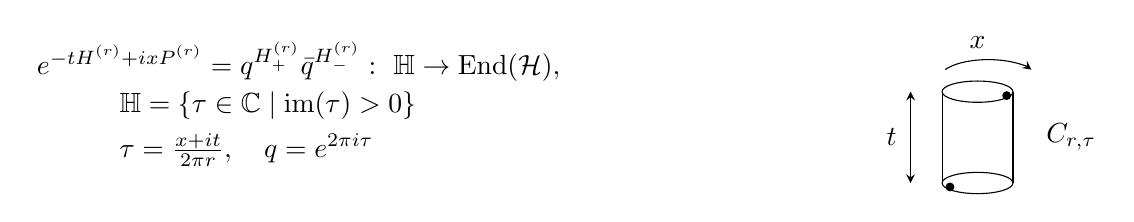
\begin{tikzpicture}[baseline=(current bounding box.center), >=stealth]
  \node[anchor=west] (a) at (0,0.62) {$e^{-tH^{(r)}+ixP^{(r)}}=q^{H^{(r)}_+}\bar q^{H^{(r)}_-}:\ \HH\to\mathrm{End}(\cH),$};
  \node[anchor=west] (b) at (1.05,0.06) {$\HH=\{\tau\in\C\mid\operatorname{im}(\tau)>0\}$};
  \node[anchor=west] (c) at (1.05,-0.50) {$\tau=\frac{x+it}{2\pi r},\quad q=e^{2\pi i\tau}$};
  \draw (11.62,-0.92) -- (11.62,0.24);
  \draw (12.52,-0.92) -- (12.52,0.24);
  \draw (12.07,0.24) ellipse (0.45 and 0.135);
  \draw (12.07,-0.92) ellipse (0.45 and 0.135);
  \fill (12.44,0.19) circle (1.6pt);
  \fill (11.72,-0.97) circle (1.6pt);
  \draw[<->] (11.22,-0.92) -- (11.22,0.24);
  \node at (10.98,-0.34) {$t$};
  \draw[->] (11.66,0.52) arc (152:28:0.62 and 0.24);
  \node at (12.07,0.86) {$x$};
  \node[anchor=west] at (12.82,-0.34) {$C_{r,\tau}$};
\end{tikzpicture}
\tag{39}
\end{equation}
它推广了量子力学中的时间演化半群 (6)，其中（为后文方便）引入算子 [Wit86, Eq. 106]
\begin{equation}
H^{(r)}_+=\frac r2\left(H^{(r)}+P^{(r)}\right),\qquad H^{(r)}_-=\frac r2\left(H^{(r)}-P^{(r)}\right).
\tag{40}
\end{equation}

% [Tutor Note: (39) 右侧的圆柱示意（高 $t$、旋转 $x$、两个标记点、标签 $C_{r,\tau}$）用内联 TikZ 重绘，它是公式的一部分而非编号图，故不用 \figomit；原图的两点标出粘合时两个边界点的对应。]
% [Tutor Note: 谱的关系可验证：由 (40) 得 $H^{(r)}_++H^{(r)}_-=rH^{(r)}$、$H^{(r)}_+-H^{(r)}_-=rP^{(r)}$，故 $rP^{(r)}$ 的谱为 $\Z+\frac n{24}$、$H^{(r)}_\pm$ 的谱为 $\frac12\left(\lambda\pm(k+\frac n{24})\right)$，这正是 (50) 与图 6 两条轴标注的来源。]
% [Tutor Note: $n$ 在此首现而未加说明（到例 4.3 才明确 $n=\dim M$）；原文即如此，读者可先把它读作理论的次数。]

正如 (39) 右方所示，可以把这一半群表示几何地重新表述：参数 $(r,\tau)$ 确定一个圆柱 $C_{r,\tau}$，它被看作半径为 $r$ 的圆周之间的一条欧几里得（即平坦 Riemann）配边，其中复参数 $\tau$ 编码圆柱之高 $t$，以及度量两个边界圆周参数化之差的旋转 $x\bmod 2\pi r$ [Wit86, Figure 2]。\emph{配分函数}是半群表示 (39) 的特征（character，即迹），
\[
Z(r,\tau):=\Tr\left(q^{H^{(r)}_+}\bar q^{H^{(r)}_-}\right)\in C^\infty(\R_{>0}\times\HH),\qquad r\in\R_{>0},\ \tau\in\HH.
\]

路径积分论证 [Wit86, §3] 把 $Z(r,\tau)$ 与理论在环面上的取值等同起来，该环面为 $T_{r,\tau}=\R^2/(2\pi r\Z\oplus 2\pi\tau\Z)$，由把圆柱两端粘合而成。一般的不变性使人期待这一取值只依赖于底层的% [原文 p.21]
环面，而不依赖于由 $r$ 与 $\tau$ 生成的带基格。群 $\mathrm{SL}_2(\Z)$ 通过改变此格的基而作用，
\[
\begin{bmatrix} a & b\\ c & d \end{bmatrix}\cdot(r,\tau)=\left(r|c\tau+d|,\ \frac{a\tau+b}{c\tau+d}\right),\qquad \begin{bmatrix} a & b\\ c & d \end{bmatrix}\in\mathrm{SL}_2(\Z)
\]
于是朴素地，人们可能期待 $Z(r,\tau)$ 是 $\mathrm{SL}_2(\Z)$-不变的函数。然而，追踪 $P^{(r)}$ 的谱中 $n/24r$ 的平移，可见 $Z(r,\tau)$ 只在一个由特征标 $\chi^n\colon\MP_2(\Z)\to\C^\times$ 编码的单位根的意义下不变 [Wit87]
\begin{equation}
Z(r,\tau)\in C^\infty(\R_{>0}\times\HH;\chi^n)^{\MP_2(\Z)}
\tag{41}
\end{equation}
其中 $\MP_2(\Z)\to\mathrm{SL}_2(\Z)$ 是 metaplectic 二重覆盖。$Z(r,\tau)$ 不能 $\mathrm{SL}_2(\Z)$-不变，这是反常理论的一个标志 [Fre87, §4]。事实上，$Z(r,\tau)$ 决定了欧几里得环面上 Pfaffian 线丛的第 $n$ 次张量幂的一个截面，而该线丛的截面与权 $n/2$ 的模形式密切相关；见注 4.1。

% [Tutor Note: (41) 记号的读法：$C^\infty(\R_{>0}\times\HH;\chi^n)$ 是取值于线丛 $\chi^n$ 的截面空间，上标 $\MP_2(\Z)$ 取 $\MP_2(\Z)$-不变部分；$\chi^n$ 即 (45) 中特征标 $\chi$ 的 $n$ 次幂（$n$ 次张量幂 $\leftrightarrow$ 权 $n/2$），与 (49) 一致。]

接下来加入超对称：\footnote{本讨论只考虑 Ramond 扇区；在 §4.3 中我们会纳入 Neveu--Schwarz 扇区。} $H^{(r)}_+$ 的 $\mathcal N_+$ 个奇的交换平方根、与 $H^{(r)}_-$ 的 $\mathcal N_-$ 个奇的交换平方根，这些数据称为 $\mathcal N=(\mathcal N_+,\mathcal N_-)$ \emph{超对称}。 我们将关注 $\mathcal N=(0,1)$ 超对称，即单个奇算子 $Q^{(r)}$，满足
\begin{equation}
(Q^{(r)})^2=\frac12[Q^{(r)},Q^{(r)}]=H^{(r)}_-,\qquad [Q^{(r)},P^{(r)}]=[Q^{(r)},H^{(r)}]=0.
\tag{42}
\end{equation}

推广超对称量子力学中的时间演化 (26)，算子 $Q^{(r)}$ 把半群表示 (39) 提升为一个\emph{超半群}（supersemigroup）表示
\begin{equation}
q^{H^{(r)}_+}\bar q^{H^{(r)}_-+\sqrt{2\pi i}\,\theta Q^{(r)}},\qquad \mathbb H^{2|1}\to\mathrm{End}(\cH)
\tag{43}
\end{equation}
其中 $\HH^{2|1}\subset\R^{2|1}$ 是超 Lie 群 $\R^{2|1}$ 的上半空间，其乘法为
\begin{equation}
(\tau',\bar\tau',\theta')\cdot(\tau,\bar\tau,\theta)=(\tau'+\tau,\ \bar\tau'+\bar\tau+\theta'\theta,\ \theta'+\theta),\qquad (\tau',\bar\tau',\theta'),(\tau,\bar\tau,\theta)\in\R^{2|1}.
\tag{44}
\end{equation}
这一超半群表示同样可以几何地解释，但此时是作为某个\emph{超圆柱}（super cylinder）范畴的表示，其几何参数为 $(r,\tau,\bar\tau,\theta)\in\R_{>0}\times\HH^{2|1}$。类似地，该半群表示的迹对应理论在\emph{超环面}（super torus）上的取值，这施加一个与 (41) 类似的预期不变性。这一几何示意地画在图 5 中。

% [Tutor Note: $\sqrt{2\pi i}$ 在原文里只覆盖 $2\pi i$，$\theta Q^{(r)}$ 在根号之外；这是超半群上 $q^{H_+}\bar q^{H_-+(\text{odd})}$ 的标准写法，不要误读成 $\sqrt{2\pi i\,\theta Q^{(r)}}$。]
% [Tutor Note: 原文第 9 号脚注（本译本第 2 号脚注）只考虑 Ramond 扇区；Neveu--Schwarz 扇区要到 §4.3（c05 块）才纳入，故本块的 $\mathcal N$ 只指 Ramond 侧。]

% [原文 p.21]
\figomit{5}{半群中的复合对应圆柱的粘合，而环面上的取值对应迹。}

\begin{remark}[4.1]
考虑分类带奇 spin 结构的 spin 椭圆曲线的商叠 $\HH/\!/\MP_2(\Z)$，其中 $\MP_2(\Z)$ 经二重覆盖 $\MP_2(\Z)\to\mathrm{SL}_2(\Z)$ 以分式线性变换作用在 $\HH$ 上。该叠上有一个线丛，它由如下特征标确定：
\begin{equation}
\chi\colon\MP_2(\Z)\to\MP_2(\Z)/[\MP_2(\Z),\MP_2(\Z)]\simeq\Z/24\hookrightarrow\C^\times
\tag{45}
\end{equation}
\end{remark}

% [Tutor Note: 原文注 4.1 在式 (45) 处收尾，p22 另起一段、用正体 "which is the Pfaffian line bundle…" 接着把这句话说完；中译为免段落以关系从句开头，在 p22 段首改写为「这一线丛就是……」，语义未变。]
% [Tutor Note: 记号 $\HH/\!/\MP_2(\Z)$ 表示作用群胚的商（作用非自由之处保留稳定化子），与轨道空间 $\HH/\MP_2(\Z)$ 不同；该商是分类 spin 椭圆曲线的模叠。]

% [原文 p.22]
这一线丛就是 Pfaffian 线丛 $\mathrm{Pf}\to\HH/\!/\MP_2(\Z)$ [Fre87, §4]。另一个线丛的截面是权 $1/2$ 的模形式，即满足
\begin{equation}
f\left(\frac{a\tau+b}{c\tau+d}\right)=\sqrt{c\tau+d}\,f(\tau).
\tag{46}
\end{equation}
的全纯函数 $f(\tau)$。

由 (46) 确定的线丛与 Pfaffian 线丛都是 Picard 群 $\mathrm{Pic}(\HH/\!/\MP_2(\Z))\simeq\Z/24$ 的生成元，因而彼此同构。Dedekind $\eta$ 函数给出一个显式同构，特别地给出整体截面上的一个双射
\[
\Gamma(\HH/\!/\MP_2(\Z);\mathrm{Pf}^{\otimes n})\xrightarrow{\ \sim\ }\mathrm{MF}_{n/2},\qquad Z(q)\mapsto\eta(q)^n Z(q),\qquad \eta(q)=q^{1/24}\prod_{k>0}(1-q^k)
\]
这可以由 $\eta(q)$ 的标准变换性质验证。模形式与 $\HH$ 上在 $\MP_2(\Z)$ 作用下带相位变换的函数之间的这一双射，在物理文献中被广泛使用，例如 [Wit88a, Eq. 18]。

% [Tutor Note: (46) 中 $\sqrt{c\tau+d}$ 的符号取定属于 $\MP_2(\Z)$ 的额外数据（二重覆盖），单看 $\mathrm{SL}_2(\Z)$-不变性无法定出；核验方式：对 $\gamma$ 与 $-\gamma$ 取同一 $\tau$，$f$ 的值相差一个符号。]
% [Tutor Note: 上式 $\mathrm{MF}_{n/2}$ 指权 $n/2$ 的模形式空间（此处不取整模形式）；与后文 $\mathrm{MF}^{\Z}$（整模形式）区别开。乘法因子 $\eta(q)^n$ 恰是权 $n/2$ 的，故双射把带相位的函数送到真模形式。]

\begin{example}[4.2（手征理论）]
数据 (40) 在 $H^{(r)}_-=0$ 时确定一个\emph{手征}场论。\footnote{chiral 的更常见用法假定 $H^{(r)}_+=L_0$ 与 $H^{(r)}_-=\bar L_0$ 是共形场论数据的一部分，其 Virasoro 生成元为 $L_k$，且 $k\in\Z$ 时 $\bar L_k=0$。} 手征理论有一个典范的超对称扩张，即取 $Q^{(r)}=0$；于是（沿用例 3.11）手征理论是拓扑理论在 2 维的相关推广，进一步讨论见式 (56)。就目前而言，我们指出：任何手征共形场论（例如顶点算子代数的数据）都给出一个 2 维手征理论，从而给出一个超对称理论。
\end{example}

% [Tutor Note: 原文第 10 号脚注（本译本第 3 号脚注）末尾作「$\bar L_k=0$ for $k\in\Z$」，字面读则右移 Virasoro 模全为零、与 $H^{(r)}_-=\bar L_0$ 相容但过于强；常见约定是 $k>0$ 时 $\bar L_k=0$。照排不改，存疑已在回报中列出。]
% [Tutor Note: 例 4.2 说手征 $\Leftrightarrow H^{(r)}_-=0$，而由 (42) 有 $H^{(r)}_-=(Q^{(r)})^2$，故 $Q^{(r)}=0$ 是唯一可能的超对称扩张（奇数算子平方为 $0$ 强于为零）；这正是本例"典范扩张"的含义。]

\begin{example}[4.3（超对称 $\sigma$ 模型与 Witten 亏格）]
设 $M$ 是 Riemann 的 spin 流形。Witten 在 $LM$ 上的旋量丛沿 $M\hookrightarrow LM$ 的限制（按定义）是向量丛的形式幂级数 [Wit88a, Eq. 24]
\begin{equation}
\cS\otimes\left(\bigotimes_{m\ge1}\mathrm{Sym}_{q^m}(TM)\right)=\cS+q\cS\otimes TM+q^2\cS\otimes\left(TM+\mathrm{Sym}^2(TM)\right)+\cdots
\tag{47}
\end{equation}
其中 $\cS$ 是 $M$ 上的旋量丛，而 $\mathrm{Sym}_q(TM)=1+qTM+q^2\mathrm{Sym}^2(TM)+\cdots$。以 $W_k(TM)$ 记 (47) 中 $q^k$ 的系数，以 $\cH$ 记 (47) 的截面的 Hilbert 完备化。对每个 $r\in\R_{>0}$，通过
\[
Q^{(r)}|_{W_k(TM)}=D\!\!\!/\otimes W_k(TM)+\sqrt{k}/\sqrt{r},\qquad P^{(r)}|_{W_k(TM)}=k/r-n/24r,\qquad n=\dim(M)
\]
在 $\cH$ 上定义算子 $P^{(r)}$ 与 $Q^{(r)}$，其中 $D\!\!\!/$ 是 $M$ 上 $\mathrm{Cl}_{-n}$-线性的 Dirac 算子。这给出一个超对称场论的输入数据 (42)。Atiyah--Singer 指标定理计算相应半群表示的（Clifford）超迹（见注 4.4）
\begin{equation}
Z(r,\tau)=\Tr_{\mathrm{Cl}_{-n}}\left(q^{H^{(r)}_+}\bar q^{H^{(r)}_-}\right)=q^{-n/24}\sum_{k=0}^{\infty}q^k\hat A(M,W_n(TM))
\tag{48}
\end{equation}
其中 $\hat A(M,W_n(TM))$ 是扭 $\hat A$ 类（twisted $\hat A$-class）。Zagier [Zag86] 验证了：当第 1 有理 Pontryagin 类 $p_1(TM)\in H^4(M;\Q)$ 为零时，归一化配分函数 $\eta(q)^n q^{-n/24}\sum_{k=0}^\infty q^k\hat A(M,W_n(TM))$ 为权 $n/2$ 的模形式。注 4.1 随即确认：$\MP_2(\Z)$ 在 $Z(r,\tau)$ 上的作用通过一个 24 次单位根给出。
\end{example}

% [Tutor Note: **原文笔误**：(48) 及其后一句都写 $\hat A(M,W_n(TM))$，但 $W_n$ 与求和指标 $k$ 无关，级数会塌成几何级数、不可能是权 $n/2$ 的模形式；按上文对 $W_k(TM)$（即 $q^k$ 的系数）的定义，此处应为 $\hat A(M,W_k(TM))$。已照排原文，并在回报中登记 ERRATA。]
% [Tutor Note: $\mathrm{Cl}_{-n}$ 指 $\R^n$ 上由负定二次形式给出的 Clifford 代数（它线性地作用在旋量丛 $\cS$ 上），与 $\mathrm{Cl}_n$ 差一个整体符号；原文排版把 Cl 印成空心体 $\mathbb Cl$，中译统一作 $\mathrm{Cl}$。]

\begin{remark}[4.4]
Clifford 模 $V$ 上 $\mathrm{Cl}_n$-线性自同态 $T$ 的\emph{Clifford 超迹}定义为 [ST04, Definition 3.2.16]
\[
\mathrm{sTr}_{\mathrm{Cl}_n}(T)=\mathrm{sTr}(\Gamma_n\circ T),\qquad T\colon V\to V
\]
其中 $\Gamma_n=(2i)^{-n/2}e_1\cdots e_n\in\mathrm{Cl}_n$，而 $\{e_1,\dots,e_n\}$ 是 $\R^n$ 的标准基，它在包含 $\R^n\subset\mathrm{Cl}_n$ 下与 Clifford 代数的（奇）元素等同。
\end{remark}

% [Tutor Note: 这里的 sTr 是通常的超迹（偶/奇部分取迹后相减），$\Gamma_n$ 用于把 Clifford 模上的迹化成普通超迹；核验：$n$ 为偶数时 $\Gamma_n$ 与 $\mathrm{Cl}_n$ 的偶部交换，故 sTr 对 Clifford 线性的 $T$ 有定义。]

% [原文 p.23]
\figomit{6}{$\qft^n$ 中的一个对象确定一个从 $\R_{\ge0}$ 到 $\R^2$ 中构形的连续映射，其标号是子空间 $\cH(k)_\lambda\subset\cH_n$，由 $k\in\Z$ 与 $\lambda\in\R$ 编号，其中 $P^{(r)}$ 与 $H^{(r)}$ 共享一个特征子空间，特征值分别为 $k/r+n/24$ 与 $\lambda$。把这些特征子空间排在平面中是方便的：横轴为 $rP^{(r)}$ 的特征值，纵轴为 $H^{(r)}_-$ 的特征值（即能量与动量之差）。超对称随即要求纵向的特征值非负，并给每个标号配上一个由 $Q^{(r)}$ 限制到 $\cH(k)_\lambda$ 得到的奇算子。这样对每个 $k\in\Z$ 都得到图 3 的一个副本。}

\begin{remark}[4.5]
有若干正在进行的工作，试图用分析工具严格构造环路空间上的旋量丛及其伴随的 Dirac 算子，使得限制到常值环路时回到例 4.3，例如见 [ST05, KM13, KM15, KLW22, LW23, Lud23]。更代数的方法则在常值环路的形式邻域中构造了密切相关的对象，例如 [GMS00, GMS04, Cos10, Cos11]。
\end{remark}

\subsection{2 维场论的逼近范畴}

下面我们给出 2 维量子场论的一些初步（且不完整的）定义，它们汇集了上述算子 (40) 与 (42) 的数据与性质。鉴于例 4.3，我们在下面的定义中加入 Clifford 次数：对每个 $n\in\Z$ 固定一个分次 $\mathrm{Cl}_n$-模 $\cH_n$，例如对无穷维可分 Hilbert 空间 $\cH$，取 $\cH_n=\mathrm{Cl}_n\otimes\cH$。

\begin{definition}[4.6]
定义拓扑群胚 $\qft^n$：其对象是 $\cH_n$ 上满足下述条件的、$\mathrm{Cl}_n$-线性无界偶算子的连续 $\R_{>0}$-族 $\{H^{(r)}_+,H^{(r)}_-\}_{r\in\R_{>0}}$：
\begin{enumerate}[label=(\roman*)]
  \item $H^{(r)}_+$ 与 $H^{(r)}_-$ 确定自伴迹类半群表示 (39)；
  \item Clifford 超迹
  \begin{equation}
  \begin{aligned}
  Z(r,\tau)&:=\mathrm{sTr}_{\mathrm{Cl}_n}\left(q^{H^{(r)}_+}\bar q^{H^{(r)}_-}\right),\qquad Z\left(r|c\tau+d|,\frac{a\tau+b}{c\tau+d}\right)=\chi^n(\gamma)Z(r,\tau),\\[2pt]
  \gamma&=\left(\begin{bmatrix}a&b\\c&d\end{bmatrix},(c\tau+d)^{1/2}\right)\in\MP_2(\Z)
  \end{aligned}
  \tag{49}
  \end{equation}
  在由特征标 $\chi^n$（来自 (45)）指定的相位意义下是 $\MP_2(\Z)$-不变的。
\end{enumerate}
$\qft^n$ 中的态射是连续映射 $\R_{>0}\to\mathrm{PU}^\pm(\cH_n)$，它们通过共轭作用在 $H^{(r)}_\pm$ 上。
\end{definition}

% [Tutor Note: (49) 只占一个号，第二行的 $\gamma$ 是给第一行右半式用的；$\gamma$ 就是 $\MP_2(\Z)$ 的元素——二阶矩阵加半整数权因子 $(c\tau+d)^{1/2}$，这正是 $\MP_2$ 作为 $\mathrm{SL}_2(\Z)$ 二重覆盖的体现，不可漏掉。]
% [Tutor Note: 定义 4.6 (ii) 只要求 (49) 在相位 $\chi^n(\gamma)$ 下不变，而不要求严格的 $\MP_2(\Z)$-不变性；这一点在定理 4.11 的证明里被用来推出"权 $-n/2$"而非"权 $0$"。]

算子 $rP=H^{(r)}_++H^{(r)}_-$ 的谱落在离散集 $\Z+\frac{n}{24}$ 中，因此这一谱不依赖于连续参数 $r$。在同构意义下，这给出状态空间的一个分解
\begin{equation}
\cH_n\simeq\bigoplus_{k\in\Z}\cH(k),\qquad H^{(r)}_-(k):=H^{(r)}_-|_{\cH(k)}
\tag{50}
\end{equation}
使 $rP^{(r)}$ 在 $\cH(k)$ 上以 $k+\frac{n}{24}\in\Z$ 作用，而 (50) 中的 $H^{(r)}_-(k)$ 由限制定义。这样一来，$\qft^n$ 中的一个对象可以看作无穷多个量子力学% [原文 p.24]
系统的汇集，其哈密顿量为 $H^{(r)}_-(k)$，对每个动量数 $k\in\Z$ 与半径 $r\in\R_{>0}$ 各一个，其中对半径参数的依赖是连续的。\footnote{更确切地说，$H^{(r)}_-(k)$ 是哈密顿量与相应量子力学系统的一个射影 $S^1$-对称的生成元的组合，见 [Wit99, §1.3]。} 这一直观可以通过图 6 中所示算子 $H^{(r)}_+$ 与 $H^{(r)}_-$ 的构形空间描述精确化：每条竖线是一个构形，它定义一个量子力学系统，另见 [Che08, Figure 4]。

% [Tutor Note: **原文笔误**：此处作 $rP=H^{(r)}_++H^{(r)}_-$，但由 (40) 有 $H^{(r)}_++H^{(r)}_-=rH^{(r)}$、$H^{(r)}_+-H^{(r)}_-=rP^{(r)}$，故应为减号；又 $H^{(r)}_\pm$ 的谱非负（超对称要求纵向特征值非负），若取加号则谱不可能落在 $\Z+\frac n{24}$ 的离散集上。已照排原文并登记 ERRATA。]
% [Tutor Note: (50) 的分解是由 $rP^{(r)}$ 的谱离散且与 $r$ 无关、加上迹类条件得到的（原文归入"如此断言"，未给证明）；注意 $\cH(k)$ 是 $H^{(r)}_-$ 的稳定子空间，故 $H^{(r)}_-(k)$ 有意义。]

\begin{proposition}[4.7]
对每个 $n\in\Z$，存在同伦等价 $|\qft^n|\simeq\BPU^\pm(\cH_n)$。
\end{proposition}

\begin{proof}[略证]
如上所述，对每个权空间 $\cH(k)\subset\cH_n$ 我们得到哈密顿量的连续 $\R_{>0}$-族 $H^{(k)}(r)$。对每个这样的哈密顿量 $H^{(r)}_k$，存在一个把全部特征子空间送到无穷远的形变。这确定一条到基点的收缩同伦，其定义域为 $\{0\}\subset\cH_n$。对每个 $k\in\Z$ 同时施加这些同伦，$\qft^n$ 的对象空间便形变收缩到对应于图 6 中空构形的零理论。由与命题 2.7 相同的论证，得到所说的同伦型。
\end{proof}

% [Tutor Note: 略证中 $H^{(k)}(r)$ 与紧随的 $H^{(r)}_k$ 指同一族哈密顿量，原文两处写法不一致（一处下标为 $k$、一处上标为 $(r)$），照排不改；读时按"固定 $k$、随 $r$ 变化"理解即可。]

\begin{remark}[4.8]
空间 $\BPU^\pm(\cH_n)$ 有一对非平凡同伦群：$\pi_1\BPU^\pm(\cH_n)\simeq\Z/2$，以及 $\pi_3\BPU^\pm(\cH_n)\simeq\Z$。二者由一个非平凡的 $k$-不变量相连。
\end{remark}

与量子力学的情形一样，若加入超对称，$\qft^n$ 的同伦型会变得更有趣。

% [Tutor Note: $\BPU^\pm(\cH_n)$ 是射影酉群的两个连通分支（对应 $\mathrm{PU}$ 的 $\pm$，即行列式相位 $\pm1$）的分类空间；故 $\pi_1=\Z/2$ 来自这两个分支，而非 $\mathrm{PU}(\cH)$ 自身的拓扑。]

\begin{definition}[4.9]
定义拓扑群胚 $\sqft^n$：其对象是 $\mathrm{Cl}_n$-线性无界算子的连续 $\R_{>0}$-族 $\{H^{(r)}_+,Q^{(r)}\}_{r\in\R_{>0}}$，其中 $H^{(r)}_+$ 是偶的、$Q^{(r)}$ 是奇的。这些数据满足两条性质。
\begin{enumerate}[label=(\roman*)]
  \item $H^{(r)}_+$ 与 $Q^{(r)}$ 确定自伴迹类超半群表示 (43)。
  \item 令 $H^{(r)}_-=(Q^{(r)})^2$，则 Clifford 超迹 (49) 在由特征标 $\chi^n$（来自 (45)）指定的相位意义下是 $\MP_2(\Z)$-不变的。
\end{enumerate}
$\sqft^n$ 中的态射是连续映射 $\R_{>0}\to\mathrm{PU}^\pm(\cH_n)$，它们通过共轭作用在 $H^{(r)}_+$ 与 $Q^{(r)}$ 上。
\end{definition}

仿照定义 4.6 之后的讨论，$\sqft^n$ 中的一个对象可以看作无穷多个超对称量子力学系统的汇集，其超对称生成元为 $Q^{(r)}(k):=Q^{(r)}|_{\cH(k)}$，对每个动量数 $k\in\Z$ 与半径 $r\in\R_{>0}$ 各一个。关于构形空间的视角，我们仍参见图 6。

% [Tutor Note: 定义 4.9 里 $H^{(r)}_-$ 不再是独立数据，而是由 (ii) 取成 $(Q^{(r)})^2$；这与定义 4.6 中 $H^{(r)}_\pm$ 并列的写法不同，后者是 4.6 的子情形（$Q=0$ 即得 4.6）。]

\begin{theorem}[4.10（{[ST04, Theorem 1.0.2]} 与 {[Che08, Theorem 2.2.2]}）]
$\sqft^n$ 中对象构成的空间映入 $K_n((q))$，即表示 Tate 曲线上椭圆上同调的谱中的第 $n$ 个空间。
\end{theorem}

\begin{proof}[略证]
把 $\cH\simeq\bigoplus_{k\in\Z}\cH(k)$ 分解为 $rP^{(r)}$ 的权空间，我们得到一个奇的、$\mathrm{Cl}_n$-线性算子的 $\R_{>0}$-族 $\{Q^{(r)}(k)\}_{k\in\Z}$。对每个 $k$ 取固定半径（例如 $r=1$），这确定一个映入定理 3.10 中表示 $K_n$ 的空间的映射。半群上的迹类条件要求 $Q^{(r)}(k)$ 对充分负的 $k$ 表示零类，于是合起来得到一个映入空间 $K_n((q))$ 的映射。
\end{proof}

\begin{theorem}[4.11（{[ST04, page 46]}）]
在相差一个 $\eta(q)^n$ 的归一化的意义下，配分函数定义一个从 $\sqft^n$ 的对象空间到（离散的）权 $-n/2$ 整模形式集合的连续映射。
\end{theorem}

% [Tutor Note: $K_n((q))$ 中的双括号表示形式 Laurent 级数，与 $K_n$ 的系数环 $K_n[q^{-1}][[q]]$ 的区别在于允许 $q$ 的负幂无限延伸；此处"第 $n$ 个空间"指椭圆上同调谱 $\TMF$ 的 $(q)$-局部化/按 Tate 曲线 $\Spec K_n$ 的分层。]

% [原文 p.25]
\begin{proof}
导致 (32) 中 $t$-无关性的 McKean--Singer 论证，对 $\eta$ 函数归一化的配分函数给出 $\bar q$-无关性
\begin{align*}
\frac{Z(r,\tau)}{\eta(q)^n}&=\eta(q)^{-n}\Tr_A\left((-1)^Fq^{H^{(r)}_+}\bar q^{H^{(r)}_-}\right)=\eta(q)^{-n}\mathrm{sTr}_A\left(q^{H^{(r)}_+}\bar q^{H^{(r)}_-}\right)\\
&=\eta(q)^{-n}\mathrm{sTr}_A\left(q^{H^{(r)}_+}|_{\ker(H^{(r)}_-)}\right)=\eta(q)^{-n}\sum_{k\in\Z}\mathrm{sTr}_A\left(q^{H^{(r)}_+}|_{\ker(Q^{(r)})\cap\cH(k)}\right)\\
&=\eta(q)^{-n}q^{n/24}\sum_{k\in\Z}q^k\mathrm{sdim}_{\mathrm{Fer}_n}\left(\ker(Q^{(r)})\cap\cH(k)\right)\\
&=\left(\prod_{k>0}(1-q^k)\right)^{n}\sum_{k\in\Z}q^k\mathrm{Index}\left(Q^{(r)}|_{\cH(k)}\right)\in\Z((q)),
\end{align*}
其中我们用了分解 (50)。在上式最后一行中，$q$ 的所有幂与 $q^k$ 的系数都是整数，而半群上的迹类条件要求 $q^k$ 的系数对充分负的 $q$ 幂为零。由连续性，整幂级数 $\eta(q)^{-n}Z(r,\tau)$ 也必须不依赖于连续参数 $r\in\R_{>0}$。因此我们断定 $\frac{Z(r,\tau)}{\eta(q)^n}\in\Z((q))$。

接下来考虑 $\MP_2(\Z)$-等变性质。定义 4.9 中的等变性质决定模变换性质（见注 4.1）
\[
\eta\left(\frac{a\tau+b}{c\tau+d}\right)^{-n}Z\left(r|c\tau+d|,\frac{a\tau+b}{c\tau+d}\right)=(c\tau+d)^{-n/2}\eta(\tau)^{-n}Z(r,\tau)
\]
从而得到所说的权 $-n/2$ 整模形式。
\end{proof}

% [Tutor Note: 末行按 $\eta(q)=q^{1/24}\prod_{k>0}(1-q^k)$ 直接代入应有 $\left(\prod_{k>0}(1-q^k)\right)^{-n}$（因为 $\eta(q)^{-n}q^{n/24}=\prod(1-q^k)^{-n}$），而原文印的是正指数 $n$（已 1200dpi 复核，确无负号）；两种写法的系数都是整数，$\Z((q))$ 的结论不受影响。已照排原文，作为疑问上报。]
% [Tutor Note: 第一步把 $\Tr_A((-1)^F\cdot)$ 改写成 $\mathrm{sTr}_A(\cdot)$；第二步把超迹限制到 $\ker H^{(r)}_-$，用 $\ker H^{(r)}_-=\ker Q^{(r)}$（因 $H^{(r)}_-=(Q^{(r)})^2$ 且 $Q$ 自伴）；第三步用 $\bar q$-无关性把 $\bar q$ 的依赖消掉，只留下与 $q$ 的幂次 $k$。这三步是原文"省略论证"的关节，读懂后才知为何末行只剩 Index。]

\begin{remark}[4.12]
上文中我们把模形式理解为\emph{弱全纯}模形式，即一个全纯函数 $f\in\cO(\HH)$，它在 $\mathrm{SL}_2(\Z)$ 作用下带权变换，并且当 $\tau\to i\infty$ 时至多有一个有限阶极点。
\end{remark}

设 $\chi\qft^n\subset\qft^n$ 记例 4.2 中手征场论的子群胚，即 $(H^{(r)}_+,H^{(r)}_-)=(H^{(r)}_+,0)$。

\begin{corollary}[4.13（{[ST11, Theorem 1.15]}）]
在相差一个 $\eta(q)^n$ 的归一化的意义下，配分函数定义一个从 $\chi\qft^n$ 到整模形式集合的连续映射。此外，每个整模形式都作为 $\chi\qft^n$ 中某个对象的配分函数出现，并且（特别地）作为 $\sqft^n$ 中某个对象的配分函数出现。
\end{corollary}

% [Tutor Note: 记号 $\chi\qft^n$ 里的 $\chi$ 取"chiral"首字母，指例 4.2 的手征子群胚（对象满足 $H^{(r)}_-=0$），不是 (45) 的特征标 $\chi$；两者同形不同义，读时按上下文区分。]
% [Tutor Note: 推论 4.13 的"整模形式"指 $\mathrm{MF}^{\Z}$（$q$-展开整系数），与定理 4.11 的"权 $-n/2$ 整模形式"是同一对象；本块至此结束，其证明（含式 (51)）与 Remark 4.14、式 (52) 见 c05 块。]

% sec4b.tex — c05｜原文 p25（Corollary 4.13 的证明起）–p30（References 之前）｜§4.3–§4.5
% 公式号 (51)–(56)；编号环境 4.14–4.21
% 块边界：本块从 p25 上 Corollary 4.13 的 Proof 起。该推论的陈述、注 4.12，以及 p25 上半
%   命题 4.11 的证明，均在 sec4a.tex（c04）；c04 负责 (39)–(50)。
% 注 4.14 与式 (52) 位于 p26 页首（按页面位置归本块；BLOCK_TAGS 亦把 (52) 记在 sec4b）。
% 图 7 在原书浮动于 p28 顶部，图 8 浮动于 p29 顶部：两幅均不复刻。

% [原文 p.25]
\begin{proof}
第一个断言由把例 4.2 应用于命题 4.11 得到。最后一个断言由取手征理论所对应的典范超对称理论得到（见例 4.2），前提是每个整模形式都作为某个手征理论的配分函数出现。为验证这一遗留断言，设 $f(q)\in\mathrm{MF}^{\Z}$ 是权为 $n/2$ 的模形式。若 $n$ 为奇数，则 $f(q)=0$，可取零理论作为我们的手征理论。若 $n$ 为偶数，则考虑 $f(q)\eta^n=q^{n/24}\sum a_nq^n\in q^{n/24}\Z((q))$。定义
\begin{equation}
\cH(k)=(\mathrm{Cl}_2\C^{1|1})^{\otimes n/2}\otimes\C^{\times a_n},
\qquad
H^{(r)}_+=\bigoplus_{k=-1}^{\infty}\frac{1}{r}\left(k+\frac{n}{24}\right)\cdot\id_{\cH(k)}
\tag{51}
\end{equation}
其中 $\mathrm{Cl}_2(\C^{1|1})_{\C}$ 是实现 $\mathrm{Cl}_2$ 与 $\C$ 之间 Morita 等价的双模。这个双模的 Clifford 超迹等于 1，故（利用张量积之迹的乘性）理论 (51) 的配分函数为
\[
\begin{aligned}
Z(r,\tau)
&:=\Tr_{\mathrm{Cl}_n}\left(q^{H^{(r)}_+}\bar q^{H^{(r)}_-}\right)
=\Tr_{\mathrm{Cl}_n}\left(q^{H^{(r)}_+}\right)\\
&=\sum_{k\in\Z}\Tr_{\mathrm{Cl}_n}\left((\mathrm{Cl}_2\C^{1|1})^{\otimes n/2}\right)\cdot\Tr\left(q^{k+n/24}\cdot\id_{\C^{\times a_n}}\right)
=q^{n/24}\sum_{k\in\Z}a_kq^k,
\end{aligned}
\]
它在 $\MP_2(\Z)$-作用下按 $n$ 次单位根变换，这里用到 $f(q)$ 的模性与注 4.1。
\end{proof}
% [Tutor Note: 式 (51) 右式的下指标原文印作 $k=-1$，但 $\cH(k)$ 的定义与 $k$ 无关，且同一段的分拆与下面的配分函数求和都遍历 $k\in\Z$；此下指标疑为 $k\in\Z$（或 $k=-\infty$）之误，照排不改，已登记 ERRATA。]
% [Tutor Note: 式 (51) 中的 $\C^{\times a_n}$ 表示 $a_n$ 个 $\C$ 的直和，故 $\Tr(q^{k+n/24}\id_{\C^{\times a_n}})=a_n$，这与下一行给出的系数 $a_k$ 相符，可用来核对记号。]
% [Tutor Note: 式 (51) 里花体 $\cH(k)$ 与斜体 $H^{(r)}_+$ 是两个不同对象：前者是权空间，后者是圆周长 $2\pi r$ 上的哈密顿量，$\frac1r(k+\frac n{24})$ 即第 $k$ 个 Fourier 模的能级加 Casimir 项。]
% [Tutor Note: 式 (51) 中印作 $(\mathrm{Cl}_2\C^{1|1})^{\otimes n/2}$，紧接的正文却把同一双模记作 $\mathrm{Cl}_2(\C^{1|1})_{\C}$（左 $\mathrm{Cl}_2$、右 $\C$）；两种写法指同一个 Morita 双模。]

% [原文 p.26]
% 注 4.14 全文位于本页页首（含式 (52)），紧接上一页的推论 4.13 证明，归本块。
% [Tutor Note: 注 4.14 引 [GPPV21, Table 2]，但本综述全文没有实体表格（既无 Table 1 也无 Table 2），亦无表格环境；照译该引用、不补表，读者应到 [GPPV21] 原文中查表。]
\begin{remark}[4.14]
推论 4.13 敲响了警钟：边缘同态
\begin{equation}
\pi_*\TMF\to\mathrm{MF}^{\Z}
\tag{52}
\end{equation}
从 TMF 的系数到整模形式，不是满射 [Hop02, Proposition 4.6]。因此，若猜想 1.1 要成立，就不应把全部整模形式都实现为超对称场论的配分函数。特别地，若采用定义 4.9，猜想 1.1 是假的。值得注意的是，物理中最确凿的那些超对称场论例子都与 (52) 的像一致，例如见 [GPPV21, Table 2]。然而，把给定的整模形式实现为一段场论故事这一问题，在物理文献中尚未完全解决，见 [LP23]。数学上的预期是：某些（手征）理论无法按下文 §4.5 的意义向下扩张，而向下扩张未必唯一。这既使某些模形式无法实现为配分函数，也使给定的模形式可以有多种方式实现为某个场论的配分函数。这一预期与 (52) 既不满射也不单射相符。
\end{remark}
% [Tutor Note: 注 4.14 与推论 4.13 并不矛盾：4.13 只断言每个整模形式可由定义 4.9 的（手征）理论实现；4.14 指出定义 4.9 若当作猜想 1.1 的场论，就要求 $\pi_*\TMF\to\mathrm{MF}^{\Z}$ 满射，而它不满射；弥合这一落差正是 §4.5 的向下扩张。]
% [Tutor Note: 「边缘同态」在这里指谱的系数到同伦群/模形式的边缘映射，与 §2–§3 中把上同调理论送到系数的边缘映射同义；它不满射是 TMF 与整模形式之间真实的差异，不是定义 4.9 的记号问题。]

\subsection{重新包装为配边范畴的表示}
可以把定义 4.6 与 4.9 中的分析数据重新包装，分别作为配边范畴 $\EBord_2$ 与 $\EBord_{2|1}$ 的表示的一部分。下面简要回顾这些配边范畴，细节参见 [ST11]。

$\EBord_2$ 的对象是带度量的圆周 $S^R_r$ 与 $S^{\mathrm{NS}}_r$ 的有限不交并，并带 spin 结构；其中 $r\in\R_{>0}$ 记录半径，$R$ 代表 Ramond（别名：周期的、奇的、或非边界的）spin 结构，$\mathrm{NS}$ 代表 Neveu–Schwarz（别名：反周期的、偶的、或边界的）spin 结构。$\EBord_2$ 的态射是带 spin 结构与测地边界的平坦 2-流形，如图 7 所示。除图 5 中的柱面与环面之外，改变柱面的源与目标数据就给出图 7 中的「通心粉」。由 §4.1 开头的讨论，固定源与目标的欧几里得通心粉的模空间是 $\HH/r\Z$，其中 $r\in\R_{>0}$ 记录半径，$\tau=\frac{x+it}{2\pi r}\in\HH$ 给出柱面的高度 $t$，而 $x$ 是边界参数化之差。复合对应于 $\HH$ 中的加法，例如 $C^R_{r,\tau}\circ C^R_{r,\tau'}\simeq C^R_{r,\tau+\tau'}$。环面 $\C/2\pi r\Z\oplus2\pi\tau\Z$ 上有 4 个 spin 结构。metaplectic 群 $\MP_2(\Z)$ 的作用置换三个偶 spin 结构，而奇 spin 结构在此作用下保持不变。我们强调，平坦度量排除了亏格更高的闭曲面。平坦度量连同测地边界排除了不同尺寸、或不同条数的圆周之间的配边，例如裤子不是 $\EBord_2$ 中的态射。
% [Tutor Note: $\MP_2(\Z)$ 是 $\mathrm{SL}_2(\Z)$ 的二重覆盖（metaplectic 群）；权为半整数的模形式在其上变换，而 (52) 中的整模形式权为整数、只在 $\mathrm{SL}_2(\Z)$ 上变换。本条与证明末「按 $n$ 次单位根变换」相呼应。]
% [Tutor Note: 环面上的 4 个 spin 结构按「偶/奇」分为 3+1：三个偶（可边界）结构被 $\MP_2(\Z)$ 置换，奇结构固定。这里的奇/偶与 $R$/$\mathrm{NS}$ 的别名「奇/偶」一致，勿与 $\Z/2$-分次混同。]

加上超对称，$\EBord_{2|1}$ 的对象是 $1|1$ 维超圆周；其模空间同样由 spin 结构与半径参数化 [BE23c, §4.5]，故沿用同一记号 $S^R_r,S^{\mathrm{NS}}_r\in\EBord_{2|1}$。它们之间的配边是带测地边界的 $2|1$ 维欧几里得流形。与 $1|1$ 维情形类似，这在 $\EBord_{2|1}$ 的态射模空间中引入奇方向。例如，Ramond 扇区中的超欧几里得柱面由 $\R_{>0}\times\HH^{2|1}$ 参数化，其复合为
\begin{equation}
C^R_{r,\tau,\bar\tau,\theta}\circ C^R_{r,\tau',\bar\tau',\theta'}\simeq C^R_{r,\tau+\tau',\bar\tau+\bar\tau'+\theta\theta',\theta+\theta'},
\qquad r\in\R_{>0},\ (\tau,\bar\tau,\theta)\in\HH^{2|1}.
\tag{53}
\end{equation}
这给出超半群（supersemigroup）表示 (43) 的几何对应物。
% [Tutor Note: (53) 中 $\bar\tau$ 的平移量 $\theta\theta'$ 是 $\HH^{2|1}$ 半群乘法的奇-奇项，$\theta$ 的平移量则是 $\theta+\theta'$；把它与式 (43) 的代数侧逐项对照，可确认「柱面的复合」与「超半群乘法」是同一结构的两面。]

为建立与猜想 1.1 相关的次数 $n$ 超欧几里得场论，首先必须描述次数扭。以 $\mathrm{Cl}(L_r\R^n)$ 记向量空间 $L_r\R^n=C^\infty(S^1_r;\R^n)$ 关于双线性配对 $\int_0^{2\pi r}\langle\psi(t),\varphi(t)\rangle dt$ 的 Clifford 代数。$S^1_r$ 在 $L_r\R^n$ 上的旋转作用保持此双线性配对，从而给出 $\mathrm{Cl}(L_r\R^n)$ 上由代数自同构构成的 $S^1_r$-作用。对每个 $\tau\in\HH/r\Z$，存在代数映射 $\varphi_r(\tau)\colon\mathrm{Cl}(L_r\R^n)\to\mathrm{Cl}(L_r\R^n)$，它由该 $S^1_r$-作用的解析延拓得到。细节参见 [ST11, page 59]。

% [原文 p.27]
\begin{definition}[4.15（次数扭，仅 Ramond 扇区的略述）]
次数扭的取值是
\begin{equation}
\begin{gathered}
\alpha_n\colon\EBord_{2|1}\to\Alg,\\
\alpha_n(S^R_r)=\mathrm{Cl}(L_r\R^n),\\
\alpha_n(C^R_{r,\tau,\bar\tau,\theta})={}_{\varphi_r(\tau)\mathrm{Cl}(L_r\R^n)}\mathrm{Cl}(L_r\R^n)_{\mathrm{Cl}(L_r\R^n)},\\
\alpha_n\Big(\,\tikz[baseline=-0.35ex,line width=0.35pt,scale=0.32]{
\draw (0,0) ellipse (0.42 and 0.18);
\draw (2.2,0) ellipse (0.42 and 0.18);
\draw (0,0.14) .. controls (0.35,1.0) and (1.85,1.0) .. (2.2,0.14);
\draw (0.42,0.12) .. controls (0.75,0.75) and (1.45,0.75) .. (1.78,0.12);
\node[anchor=base west,inner sep=1.4pt] at (2.62,0.02) {$\scriptstyle r,\tau,\bar\tau,\theta$};
}\,\Big)=\mathrm{Cl}(L_r\R^n)_{\varphi_r(\tau)\mathrm{Cl}(L_r\R^n)\otimes\mathrm{Cl}(L_r\R^n)},\\
\alpha_n\Big(\,\tikz[baseline=-0.35ex,line width=0.35pt,scale=0.32]{
\draw (0,0) ellipse (0.42 and 0.18);
\draw (2.2,0) ellipse (0.42 and 0.18);
\draw (0,-0.14) .. controls (0.35,-1.0) and (1.85,-1.0) .. (2.2,-0.14);
\draw (0.42,-0.12) .. controls (0.75,-0.75) and (1.45,-0.75) .. (1.78,-0.12);
\node[anchor=base west,inner sep=1.4pt] at (2.62,-0.02) {$\scriptstyle r,\tau,\bar\tau,\theta$};
}\,\Big)={}_{\varphi_r(\tau)\mathrm{Cl}(L_r\R^n)\otimes\mathrm{Cl}(L_r\R^n)}\mathrm{Cl}(L_r\R^n),\\
\alpha_n\Big(\,\tikz[baseline=-0.35ex,line width=0.35pt,scale=0.32]{
\draw (0,0) circle (0.48);
\draw (0,0) circle (0.24);
\node[anchor=base west,inner sep=1.4pt] at (0.62,0) {$\scriptstyle r,\tau,\bar\tau,\theta$};
}\,\Big)=\mathrm{Pf}^{\otimes-n}
\end{gathered}
\tag{54}
\end{equation}
其中所有模都来自 $\mathrm{Cl}(L_r\R^n)$ 作为其自身的双模，而左作用被代数自同构 $\varphi_r(\tau)$ 扭过；$\mathrm{Pf}$ 是 Pfaffian 线丛，见注 4.1。这些取值与 $(\bar\tau,\theta)$ 无关，因此次数扭是手征的。
\end{definition}
% [Tutor Note: (54) 第 3、4、5 行的自变量，原文印的是三个手绘小配边图（无文字符号）：起拱的把手（两个边界圆 + 上拱的带）、其镜像（下凹的带）、同心双圆。译本以同构形的简笔线图复刻，只为可读性，不含原文之外的任何信息；下标 $r,\tau,\bar\tau,\theta$ 的位置照原文紧跟在图右侧。]
% [Tutor Note: (54) 用的是双模记号 ${}_AM_B$：左下标记左作用的扭、右下标记右作用的扭，缺省即该侧未扭。第 2 行读作 ${}_{\varphi_r(\tau)\mathrm{Cl}}\mathrm{Cl}_{\mathrm{Cl}}$；第 3 行（杯形把手）缺左下标、第 4 行（帽形把手）缺右下标，二者恰好把左扭与右扭对调，不可互换。]

\begin{remark}[4.16]
「超化」（superfication）函子 $\EBord_2\to\EBord_{2|1}$ [ST11, Eq. 4.14] 使人能把扭 $\alpha\colon\EBord_{2|1}\to\Alg$ 限制为扭 $\EBord_2\to\Alg$。特别地，扭 (54) 决定了 2 维欧几里得配边范畴的扭。
\end{remark}

\begin{remark}[4.17]
定义 4.15 省略了 Neveu–Schwarz 的取值，但它们来自向量空间 $C^\infty(S^1;\mu\otimes\R^n)$ 的类似 Clifford 代数，其中 $\mu$ 是 Möbius 丛，即 Neveu–Schwarz spin 结构对应的旋量丛。作为从欧几里得配边范畴出发的函子，次数扭的详细略述见 [ST11, §4.3]，另见 [Lud22]。该理论是手征的，因此预期容许一个典范的超对称扩张，推广例 4.2。然而，这一扩张在 [ST11] 的配边框架中的细节尚未做出。
\end{remark}

令 $\QFT^{\alpha}_{2|1}(\cX)$ 记 $\cX$ 上 $\alpha$-扭的反射正 $2|1$ 维欧几里得场论构成的群胚（见定义 1.9）。在存在手征超对称时，反射正性更为微妙，但最终反射结构的数据遵循与定义 2.13 类似的模式。我们先分析点上的场论之群胚 $\QFT^n_2:=\QFT^{\alpha_n}_2(\mathrm{pt})$ 与 $\QFT^n_{2|1}:=\QFT^{\alpha_n}_{2|1}(\mathrm{pt})$，其中的场论被次数扭 (54) 所扭。

\begin{hypothesis}[4.18（{[ST04, Theorem 1.0.2] [Che08, Theorem 2.2.2]}）]
存在叠的映射
\begin{equation}
\QFT^n_2\to\qft^n
\qquad\text{与}\qquad
\QFT^n_{2|1}\to\sqft^n
\tag{55}
\end{equation}
它们由限制到 Ramond 扇区得到。连同定理 4.10 与 4.11，叠 $\QFT^n_{2|1}$ 容许到表示 $K((q))$ 的谱中第 $n$ 个空间的映射，以及到整模形式集合的映射。
\end{hypothesis}
% [Tutor Note: 假设 4.18 原文 "There are map of stacks" 有语法笔误，应为 "There are maps of stacks"；中文无单复数，照译，已登记 ERRATA。]
% [Tutor Note: (55) 的两个映射都是「限制到 Ramond 扇区」，即忘掉超对称与 Neveu–Schwarz 扇区的数据；这正是注 4.14 之后所说的反例来源——配边定义严格比定义 4.9 携带更多信息（见 §4.4 开头）。]

\begin{proof}[略述]
我们聚焦于 $\QFT^n_{2|1}\to\sqft^n$；无超对称的情形更容易。

首先证明：限制到 Ramond 扇区的 (54) 的扭场论决定了通常 Clifford 代数 $\mathrm{Cl}_n$ 上的模，做法依照 [ST11, §6]。想法是按 Fourier 模，即 $S^1_r$-作用的权空间，分解代数 $\mathrm{Cl}(L_r\R^n)$。这些权给出稠密包含
\[
\mathrm{Cl}_n\otimes\bigotimes_{k>0}\mathrm{Cl}(\C^n_k\oplus\C^n_{-k})\hookrightarrow\mathrm{Cl}(L_r\R^n),
\]
其中 $\mathrm{Cl}_n$ 是 $S^1_r$-不动点（即常值映射）的 Clifford 代数，而 $\mathrm{Cl}(\C^n_k\oplus\C^n_{-k})$ 是 Fourier 数为 $k$ 与 $-k$ 的环路构成的 Clifford 代数。对配对 $\int_{S^1}\langle\varphi(t),\psi(t)\rangle dt$，这样的环路只彼此非平凡配对，且该配对是双曲配对。于是得到 Clifford 代数 $\mathrm{Cl}(\C^n_k\oplus\C^n_{-k})\subset\mathrm{Cl}(L_r\R^n)$ 作为子代数。此外，对每个 $k$，$\mathrm{Cl}(\C^n_k\oplus\C^n_{-k})\simeq\mathrm{Cl}_{n,n}$ 且 Morita 等价于 $\C$。Morita 双模的张量积的完备化给出从 $\mathrm{Cl}(L_r\R^n)$-模到 $\mathrm{Cl}_n$-模的所需函子，见 [ST11, Eq. 6.2]。

把这一点应用于 $E\in\QFT^n_{2|1}$ 在 Ramond 扇区超环带 (53) 的子范畴上的取值，得到形如 (43) 的 $\mathrm{Cl}_n$-线性超半群表示。这给出 $\sqft^n$ 中一个对象的数据。$E$ 在 Ramond–Ramond 超环面上的取值施加
% [原文 p.28]
模性条件 (49) [ST11, page 60]。应用与假设 2.14 类似的论证，扭场论之间的同构来自状态空间之间的射影同构。于是得到函子 $\QFT^n_{2|1}\to\sqft^n$。
\end{proof}
% [Tutor Note: 稠密包含里 $\mathrm{Cl}_n$ 来自常值环路（$k=0$）；配对只把模 $k$ 与 $-k$ 配起来，每个因子 $\mathrm{Cl}(\C^n_k\oplus\C^n_{-k})$ 上的配对非退化且双曲，故它 Morita 等价于 $\C$。]
% [Tutor Note: 原文 "with of Fourier numbers $k$ and $-k$" 多一个 of，属笔误；中文不受影响，已登记 ERRATA。]

% 原书中图 7 浮动于本页顶部，上一段的句子被它隔断；为避免割裂汉语句子，图 7 的
% \figomit 置于该段之后。图 7 的正文引用见 §4.3 首段「如图 7 所示」。
\figomit{7}{$2|1$ 维配边范畴的生成元与关系，类比于图 2 与图 4，但几何参数由 $(r,\tau,\bar\tau,\theta)\in\R_{>0}\times\HH^{2|1}$ 给出。在记录好源与目标之后，复合对应于半群 $\HH^{2|1}$ 中的乘法。按惯例，配边沿正（向上）方向读。左图：把一条「悲伤通心粉」粘到一条「快乐通心粉」上，得到一个柱面。右图：把柱面粘到一条「快乐通心粉」上，得到一条「更快乐的通心粉」。}
% [Tutor Note: 图 7 内还印出两条复合关系（对应 (53) 的复合律）：左为一端粘合给出 $C^R_{r,\tau+\tau',\bar\tau+\bar\tau'+\theta\theta',\theta+\theta'}$，右为两段柱面先竖向粘合再与通心粉复合；这些式子属于图的内容，随图一并省略。]

\subsection{配边框架的更多洞见}
与假设 3.20 相反，假设 4.18 中的映射 $\QFT^n_{2|1}\to\sqft^n$ 不再是叠的满射：配边定义所包含的信息严格多于定义 4.9，例如 $E(S^{\mathrm{NS}}_r)$ 在 Neveu–Schwarz 扇区上的取值。下面强调若干进一步的增强。

\begin{example}[4.19（实结构）]
在 [ST11] 的配边框架中，$\EBord_{2|1}(\cX)$ 的对象与态射都构成叠，意思是配边的等距群被编码在结构之中。这导致对象上一个在 1 维情形中不存在的额外 $\Z/2$-自同构，归根结底是因为 $-\id\in\mathrm{O}_2$ 是 $\R^2$ 的保向等距（与 $\R$ 上反转定向的 $-1\in\mathrm{O}(1)$ 形成对照）。物理上，这个自同构是宇称–时间反演。对反射正的理论，这个对称性决定状态空间与其复共轭之间的同构，即一个实结构的数据 [BE23c, §8.4]，从而把 4.18 中取值于 $K((q))$ 的上闭链映射细化为取值于 $\KO((q))$ 的映射。这一论证也可以用物理语言理解，见 [Wit87] 与 [GPPV21, 3.2.2]。
\end{example}
% [Tutor Note: 关键在行列式：$-\id\in\mathrm{O}_2$ 的行列式为 $(-1)^2=1$，故保向；而 $-1\in\mathrm{O}(1)$ 的行列式为 $-1$，反转定向。保向的额外自同构才允许它在反射正理论里给出状态空间到其复共轭的同构，从而把 $K((q))$ 细化为 $\KO((q))$。]

\begin{example}[4.20（场论的挠不变量）]
沿用注 3.25，由 $\EBord_{2|1}(\cX)$ 编码的超模空间可能相当微妙。特别地，带映入 $\cX$ 的映射的超欧几里得环面的模空间出乎意料地丰富。当 $\cX=X$ 为光滑流形时，[BE23a] 证明了该模空间上的函数决定 $H(M;\mathrm{MF})$ 中一个类的上闭链代表，即取值于模形式的通常上同调。超环面模空间的微妙特征在上闭链代表中编码全纯反常消去数据，从而恢复物理讨论 [GJFW21, GJF23] 所预期的信息。连同 Witten 对超对称 $\sigma$ 模型的局部构造（见例 4.3），这些反常消去数据可用于给出 Bunke 与 Naumann 的 $4k-1$ 维 string 流形挠不变量的一个量子场论解释 [BN14]。这些想法在 [BE23c] 中被置于 [ST11] 的框架之中，给出由 2 维超对称场论捕捉到的 TMF 挠的首批例子。
\end{example}
% [Tutor Note: 本段写 "For $\cX=X$ a smooth manifold"，与 §1 末尾同样的记号混用（前一个 $\cX$ 是叠）；照译作 $\cX=X$，已登记 ERRATA。]
% [Tutor Note: 上闭链所在的上同调原文写作 $H(M;\mathrm{MF})$，但本段通篇以 $X$ 记流形、$M$ 未定义；疑为 $H(X;\mathrm{MF})$ 之误，照排不改，待与 [BE23a] 原文核对（已记入回报）。]

% [原文 p.29]
\figomit{8}{全扩张的 $2|1$ 维欧几里得配边范畴中 2-态射的水平复合。条带 $S_{\ell,\tau,\bar\tau,\theta}$ 由入射弦与出射弦的长度、以及 $\HH^{2|1}\subset\R^{2|1}$ 中一个刻画条带角度与高度的参数所标定。文中把它们视为沿向上（时间）方向传播的开弦，并带有沿水平（空间）方向的粘合操作。把一条条带的边界粘合起来，就回到先前考虑过的柱面范畴。}

\begin{example}[4.21（次数扭与椭圆 Thom 类的对称性）]
与例 3.15 类似，定义 4.15 的次数扭可以构造为 $n$ 个手征自由费米子理论的量子化 [ST04, §2.6]，该理论由场与作用量泛函
\[
\psi\in\Gamma(\Sigma;\cS\otimes\R^n),
\qquad
S(\psi)=\frac{1}{2}\int_\Sigma\langle\psi,\bar\partial\psi\rangle
\]
定义，其中 $\Sigma$ 是带旋量丛 $\cS\to\Sigma$ 与手征 Dirac 算子 $\bar\partial$ 的 spin Riemann 面。该理论具有由映射 $\Sigma\to\mathrm{O}(n)$ 给出的经典（规范）对称性，作用方式为把 $\psi$ 在 $\R^n$ 中旋转。在量子理论中，这导致环路群 $L\mathrm{O}(n)$ 在状态 Hilbert 空间上的射影作用，它与 Clifford 代数 $\mathrm{Cl}(L\R^n)$ 的作用交织。这个环路群表示正是 $\widetilde{L\mathrm{Spin}}(n)$ 的级别 1（level one）表示的费米子 Fock 空间构造，其中 $\widetilde{L\mathrm{Spin}}(n)$ 是环路群 $L\mathrm{Spin}(n)$ 由 $p_1/2\in H^4(B\mathrm{Spin}(n);\Z)$ 分类的中心扩张 [PS86, §12]。这个手征共形场论决定一个具有 $\mathcal N=(0,1)$ 超对称的欧几里得场论。在猜想 1.1 之下，预期它恢复泛椭圆 Thom 类，见 [ST04, Theorem 1.0.3] 与 [DH11]。
\end{example}
% [Tutor Note: $p_1/2$ 取整性：$p_1$ 是 $B\mathrm{SO}(n)$ 的整类，拉回到 $B\mathrm{Spin}(n)$ 后被 2 整除，故 $p_1/2\in H^4(B\mathrm{Spin}(n);\Z)$，它正是该中心扩张的分类类。]
% [Tutor Note: 「泛椭圆 Thom 类」指与定义 4.15 的次数扭相配的 Thom 类，其在 string 定向下的取值为椭圆亏格；例 4.21 的作用是把这一几何对象实现为自由费米子场论，这正是 §4.5 中全扩张场论要恢复的对象。]

\subsection{最后的边疆：向下扩张}
全扩张的 $2|1$ 维欧几里得配边 2-范畴编码带角 $2|1$ 维超欧几里得流形的切割与粘合：由图 7 中的操作所编码的闭弦理论被细化为图 8 所描绘的开弦理论。预期是：向下扩张会把假设 4.18 中描述的取值于 $\KO((q))$ 与 $\mathrm{MF}^{\Z}$ 的不变量，细化为取值于 TMF 的场论不变量，即 (1) 中的上闭链映射。

这类全扩张场论的一些粗略特征已知，例如 [Moo03, 3.5] 与 [Seg01, §4]。然而仍有许多谜团：向下扩张不是唯一确定的，且尚无候选定义被详细写出。按惯例，这项工作可分为两个相互关联的部分：(i) 配边 2-范畴的几何；(ii) 目标 3-范畴的分析。$n$ 重 Segal 空间的语言提供了一个有前景的框架，可用来研究一般的全扩张配边范畴（例如见 [JFS17, GP20]），特别是全扩张的 $2|1$ 维欧几里得配边。目标的一个候选是共形网的对称幺半 3-范畴 [DH11, BDH15, BDH17, BDH19, BDH18]，不过预期需要一些技术性修改，因为这个 3-范畴并不去环（delooping）定义 1.5 与 [ST11] 中 1-扩张场论的 2-范畴 $\Alg$。

% [原文 p.30]
指导向下扩张中种种选择的一条途径，是更好地把握例子。或许最根本的例子是次数扭 (54) 及其与椭圆 Thom 类的预期联系，如例 4.21 所勾勒。它推广了 K 理论中已知的结构，见例 3.15。确实，一个实现如下形式的泛扭 Thom 同构的全扩张次数 $n$ 场论
\[
\QFT^{k}_{2|1}\left(\mathrm{pt}/\!/^{\nabla}\mathrm{O}(n)\right)\to\QFT^{n+k+\lambda}_{2|1}\left(\R^n/\!/^{\nabla}\mathrm{O}(n)\right)_c,
\qquad
E\mapsto E\boxtimes\Th_n
\]
将自动从 2 维超对称场论构造出一个 string 定向的可乘上同调理论。依照 Lurie 在 [Lur09b, §5.5] 中的建议，场论中的高阶等变结构随后可用来构造与 TMF 的比较，如 (1) 中那样。高阶等变性的证据来自如下预期：自由费米子场论的对称性是 string 2-群 [ST04, DH, SP11, Wal13]。

我们再加一个猜测。令 $\chi\QFT^{\bullet}_2\subset\QFT^{\bullet}_2$ 记次数为 $n$ 的理论中在 (55) 下的像为手征（例 4.2 意义下）者构成的子范畴。如推论 4.13 那样，预期这样的手征共形场论决定超对称的理论，从而给出一个包含
\begin{equation}
\chi\QFT^{\bullet}_2\xrightarrow{\ \text{群完备化？}\ }\QFT^{\bullet}_{2|1}.
\tag{56}
\end{equation}
与 (28) 类比，人们或可希望 (56) 实现手征场论的群完备化。确实，在 1 维，拓扑场论正是在重整化群流下不变的那些；而在 2 维，这些是手征共形理论。连同猜想 1.1，(56) 将把 TMF 实现为手征共形场论的群完备化。目前尚不清楚如何解读这一陈述，但很可能 (56) 的像中的刚性对象在猜想 1.1 中扮演重要角色，正如向量丛是 K 理论中的基本几何对象。
% [Tutor Note: (56) 的箭头标签原文为 "group completion?"，带问号，表示这是猜测而非已证的映射；译本照译作「群完备化？」。箭头因此不宜读作函子。]
% [Tutor Note: $\chi\QFT^{\bullet}_2$ 的上标用 $\bullet$，而正文说「次数为 $n$ 的理论」：$\bullet$ 表示对一切次数 $n$ 取并，逐次数的子范畴是 $\chi\QFT^{n}_2\subset\QFT^{n}_2$，与 p30 上文的 $\chi\QFT^n_2$ 记号一致。]
% [Tutor Note: 「1 维的拓扑场论恰是重整化群流下不变者」这一断言解释了为何 (56) 被视为群完备化：在 1 维，拓扑场论即完全可扩张到点的那部分；在 2 维，对应物是手征共形理论，而刚性对象（其对偶存在）扮演 K 理论中向量丛的角色。]


% ---------------------------- 参考文献 ----------------------------
\clearpage
% refs.tex — c06｜原文 p30（「References」标题）–p34｜参考文献
% 条目整条保留原文（作者/标题/期刊/卷/年/页码照原样），不译；顺序亦照原文，不增删、不合并。
% 本块无编号公式、无编号环境：check_block 期望 tags 0/0、env 0/0。
% [Tutor Note: 条目按原文逐条保留、一律不译；顺序也照原文（例如 [AS69]→[AS71]→[AS04] 并非严格字母序），不得重排。]
% [Tutor Note: 原文页眉为小型大写的 "REFERENCES"；译本按工程约定用 \section*{参考文献}，且此为全块唯一的 section 级命令。]
% [Tutor Note: 文字层把重音拆成 "´e"/"¨o"/"ˇc" 这类组合字符（Alvarez-Gaum´e、Bj¨orn、Jurˇco）；已按 p30–p34 页面图还原为 \'e、\"o、\v{c}、\ae{}。]
% [Tutor Note: 多条文献原文即无页码或出版项（[Lur19] 只有标题、[Jon87] 止于 "no. 2."、[Kit09a] 无页码）；照原文，不补。]

\section*{参考文献}
\addcontentsline{toc}{section}{参考文献}

% 版式：标签左置、条目文字悬挂对齐，与原文两栏式参考文献一致
\begin{description}[leftmargin=5.6em,labelwidth=5.2em,labelsep=0.4em,itemsep=0.5ex,parsep=0pt,topsep=0.8ex]

% [原文 p.30]
\item[\textbf{[AB02]}] M. Ando and M. Basterra, \textit{The Witten genus and equivariant elliptic cohomology}, Math. Z. \textbf{240} (2002), no. 4, 787--822.
\item[\textbf{[ABS64]}] M. Atiyah, R. Bott, and A. Shapiro, \textit{Clifford modules}, Topology \textbf{3} (1964), no. suppl. 1, 3--38.
\item[\textbf{[AG83]}] L. Alvarez-Gaum\'e, \textit{Supersymmetry and the Atiyah-Singer index theorem}, Communications in Mathematical Physics \textbf{90} (1983), 161--173.
\item[\textbf{[AHR10]}] M. Ando, M. Hopkins, and C. Rezk, \textit{Multiplicative orientations of $KO$-theory and the spectrum of topological modular forms}, Draft (2010).
\item[\textbf{[AKL23]}] J. Albert, J. Kaidi, and Y.-H. Lin, \textit{Topological modularity of supermoonshine}, Progress of Theoretical and Experimental Physics \textbf{2023} (2023).
\item[\textbf{[And00]}] M. Ando, \textit{Power operations in elliptic cohomology and representations of loop groups}, Transactions of the American Mathematical Society \textbf{352} (2000).
\item[\textbf{[AO21]}] M. Aganagic and A. Okounkov, \textit{Elliptic stable envelope}, J. Amer. Math. Soc. \textbf{34} (2021).
\item[\textbf{[AS69]}] M. Atiyah and I. Singer, \textit{Index theory for skew-adjoint Fredholm operators}, Inst. Hautes \'etudes Sci. Publ. Math. \textbf{37} (1969).
% [Tutor Note: 原文对“同上作者”的条目印一条长约 3em 的横线（[AS71] 前）；此处用 \rule[0.45ex]{2.6em}{0.45pt} 复刻，长度按 p30 页面图实测，且不依赖字体连字。]
\item[\textbf{[AS71]}] \rule[0.45ex]{2.6em}{0.45pt}, \textit{The index of elliptic operators IV}, Annals of Mathematics \textbf{93} (1971).
\item[\textbf{[AS04]}] M. Atiyah and G. Segal, \textit{Twisted $K$-theory}, Ukrainskyj Matematychnyj Visnyk \textbf{1} (2004).
\item[\textbf{[Ati85]}] M. Atiyah, \textit{Circular symmetry and stationary phase approximation}, Proceedings of the conference in honor of L. Schwartz, Ast\'erisque \textbf{131} (1985).
\item[\textbf{[Ati89]}] \rule[0.45ex]{2.6em}{0.45pt}, \textit{Topological quantum field theories}, Publications Math\'ematiques de l'IH\'ES \textbf{68} (1989).
\item[\textbf{[Ati90]}] \rule[0.45ex]{2.6em}{0.45pt}, \textit{The Jones-Witten invariants of knots}, S\'eminaire Bourbaki \textbf{715} (1989/90).
\item[\textbf{[BBES22]}] T. Barthel, D. Berwick-Evans, and N. Stapleton, \textit{Power operations in the Stolz--Teichner program}, Geom. Topol. \textbf{26} (2022).
\item[\textbf{[BDH15]}] A. Bartels, C. Douglas, and A. Henriques, \textit{Conformal nets I: coordinate-free nets}, Int. Math. Res. Not. \textbf{13} (2015).
\item[\textbf{[BDH17]}] \rule[0.45ex]{2.6em}{0.45pt}, \textit{Conformal nets II: conformal blocks}, Comm. Math. Phys. \textbf{354} (2017).
\item[\textbf{[BDH18]}] \rule[0.45ex]{2.6em}{0.45pt}, \textit{Conformal nets IV: the 3-category}, Algebr. Geom. Topol. \textbf{18} (2018).
\item[\textbf{[BDH19]}] \rule[0.45ex]{2.6em}{0.45pt}, \textit{Fusion of defects}, Mem. Amer. Math. Soc. \textbf{1237} (2019).
\item[\textbf{[BE23a]}] D. Berwick-Evans, \textit{Chern characters for supersymmetric field theories}, Geom. Topol. \textbf{27} (2023), no. 5, 1947--1986.
\item[\textbf{[BE23b]}] \rule[0.45ex]{2.6em}{0.45pt}, \textit{The families index for $1|1$-dimensional Euclidean field theories}, preprint (2023).
\item[\textbf{[BE23c]}] \rule[0.45ex]{2.6em}{0.45pt}, \textit{How do field theories detect the torsion in topological modular forms?}, preprint (2023).

% [原文 p.31]
\item[\textbf{[BEH16]}] D. Berwick-Evans and F. Han, \textit{The equivariant Chern character as super holonomy on loop stacks}, preprint (2016).
\item[\textbf{[BEP23]}] D. Berwick-Evans and D. Pavlov, \textit{Smooth one-dimensional topological field theories are vector bundles with connection}, Algebr. Geom. Topol. \textbf{23} (2023), no. 8, 3707--3743.
\item[\textbf{[BET19]}] D. Berwick-Evans and A. Tripathy, \textit{A model for complex analytic equivariant elliptic cohomology from quantum field theory}, preprint (2019).
\item[\textbf{[BET21]}] \rule[0.45ex]{2.6em}{0.45pt}, \textit{A de rham model for complex analytic equivariant elliptic cohomology}, Advances in Mathematics \textbf{380} (2021).
\item[\textbf{[BGV92]}] N. Berline, E. Getzler, and M. Vergne, \textit{Heat kernels and Dirac operators}, Springer, 1992.
\item[\textbf{[Bis86]}] J.-M. Bismut, \textit{The Atiyah-Singer index theorem for families of Dirac operators: Two heat equation proofs}, Inventiones mathematicae \textbf{83} (1986).
% [Tutor Note: 原文此条印作 "U. Bunke and N Naumann"，N 后确实缺句点（p31 页面图核对）；照原文保留，属原文笔误。]
\item[\textbf{[BN14]}] U. Bunke and N Naumann, \textit{Secondary invariants for string bordism and topological modular forms}, Bull. Sci. Math. \textbf{138} (2014).
\item[\textbf{[Bor92]}] R. Borcherds, \textit{Monstrous moonshine and monstrous Lie superalgebras}, Invent. Math. \textbf{109} (1992).
\item[\textbf{[BT89]}] R. Bott and C. Taubes, \textit{On the rigidity theorems of Witten}, J. Amer. Math. Soc. \textbf{2} (1989), no. 1, 137--186.
\item[\textbf{[BW97]}] S. Bates and A. Weinstein, \textit{Lectures on the geometry of quantization}, Berkeley mathematics lecture notes, American Mathematical Society, 1997.
\item[\textbf{[Che08]}] P. Cheung, \textit{Supersymmetric field theories and cohomology}, preprint (2008).
\item[\textbf{[Cos10]}] K. Costello, \textit{A geometric construction of the Witten genus I}, Proceedings of the International Congress of Mathematicians (2010).
\item[\textbf{[Cos11]}] \rule[0.45ex]{2.6em}{0.45pt}, \textit{A geometric construction of the Witten genus II}, preprint (2011).
% [Tutor Note: 标签在原文印作上标加号（DEF 后带上标 +，见 p31 页面图）；此处排作 \textbf{[DEF$^{+}$99]}，与正文引用 [DEF+99] 同指一条。]
\item[\textbf{[DEF$^{+}$99]}] P. Deligne, P. Etingof, D. Freed, L. Jeffrey, D. Kazhdan, J. Morgan, D. Morrison, and E. Witten, \textit{Quantum Fields and Strings: A Course for Mathematicians, Volume 1}, American Mathematical Society, 1999.
\item[\textbf{[Dev96]}] J. Devoto, \textit{Equivariant elliptic homology and finite groups}, Michigan Math. J. \textbf{43} (1996).
\item[\textbf{[Dev98]}] \rule[0.45ex]{2.6em}{0.45pt}, \textit{An algebraic description of the elliptic cohomology of classifying spaces}, Journal of Pure and Applied Algebra \textbf{130} (1998).
\item[\textbf{[DFHH14]}] C. Douglas, J. Francis, A. Henriques, and M. Hill, \textit{Topological modular forms}, American Mathematical Society, 2014.
\item[\textbf{[DH]}] C. Douglas and A. Henriques, \textit{Geometric string structures}, preprint.
\item[\textbf{[DH11]}] \rule[0.45ex]{2.6em}{0.45pt}, \textit{Topological modular forms and conformal nets}, Mathematical foundations of quantum field theory and perturbative string theory, Proc. Sympos. Pure Math., vol. 83, Amer. Math. Soc., Providence, RI, 2011, pp. 341--354.
\item[\textbf{[DHVW85]}] L. Dixon, J. Harvey, C. Vafa, and E. Witten, \textit{Strings on orbifolds}, Nuclear Phys. B \textbf{261} (1985).
\item[\textbf{[DM99]}] P. Deligne and J. Morgan, \textit{Notes on supermanifolds}, Quantum Fields and Strings: A Course for Mathematicians, Volume 1 (P. Deligne, P. Etingof, D. Freed, L. Jeffrey, D. Kazhdan, J. Morgan, D. Morrison, and E. Witten, eds.), American Mathematical Society, 1999.
\item[\textbf{[DMVV97]}] R. Dijkgraaf, G. Moore, E. Verlinde, and H. Verlinde, \textit{Elliptic genera of symmetric products and second quantized strings}, Comm. Math. Phys. \textbf{185} (1997).
\item[\textbf{[Dou10]}] M. Douglas, \textit{Spaces of quantum field theories}, preprint (2010).
\item[\textbf{[Dum12]}] F. Dumitrescu, \textit{$1|1$ parallel transport and connections}, Differential Geometry and its Applications \textbf{30} (2012).
\item[\textbf{[EU14]}] J. Espinoza and B. Uribe, \textit{Topological properties of the unitary group}, JP Journal of Geometry and Topology \textbf{16} (2014).
\item[\textbf{[FH21]}] D. Freed and M. Hopkins, \textit{Reflection positivity and invertible topological phases}, Geom. Topol. \textbf{25} (2021).
\item[\textbf{[FHT11a]}] D. Freed, J. Hopkins, and C. Teleman, \textit{Loop groups and twisted $K$-theory I}, J. Topol. \textbf{4} (2011), no. 4, 737--798.
% [Tutor Note: [FHT11a] 作 "J. Hopkins"、[FHT11b] 作 "M. Hopkins"，同一作者姓名缩写原文前后不一致（p31 页面图）；照原文保留。]
\item[\textbf{[FHT11b]}] D. Freed, M. Hopkins, and C. Teleman, \textit{Twisted $K$-theory and loop group representations III}, Ann. Math. \textbf{174} (2011).
\item[\textbf{[FM13]}] D. Freed and G. Moore, \textit{Twisted equivariant matter}, Ann. Henri Poincare \textbf{14} (2013).
\item[\textbf{[Fre87]}] D. Freed, \textit{On determinant line bundles}, Math. aspects of string theory (1987).
\item[\textbf{[Fre99]}] \rule[0.45ex]{2.6em}{0.45pt}, \textit{Five Lectures on Supersymmetry}, American Mathematical Society, 1999.
\item[\textbf{[Fre12]}] \rule[0.45ex]{2.6em}{0.45pt}, \textit{Lectures on twisted $K$-theory and orientifolds}, lectures at ESI Vienna (2012).
\item[\textbf{[Fre14]}] \rule[0.45ex]{2.6em}{0.45pt}, \textit{Anomalies and Invertible Field Theories}, Proc. Symp. Pure Math. \textbf{88} (2014), 25--46.
\item[\textbf{[FRV17]}] G. Felder, R. Rim\'anyi, and A. Varchenko, \textit{Elliptic dynamical quantum groups and equivariant elliptic cohomology}, Arxiv preprint (2017).
\item[\textbf{[FT14]}] D. Freed and C. Teleman, \textit{Relative quantum field theory}, Commun. Math. Phys. \textbf{326} (2014).
\item[\textbf{[Gan06]}] N. Ganter, \textit{Orbifold genera, product formulas and power operations}, Adv. Math. \textbf{205} (2006).
\item[\textbf{[Gan07]}] \rule[0.45ex]{2.6em}{0.45pt}, \textit{Stringy power operations in Tate $K$-theory}, preprint (2007).
\item[\textbf{[Gan09]}] \rule[0.45ex]{2.6em}{0.45pt}, \textit{Hecke operators in equivariant elliptic cohomology and generalized Moonshine}, Groups and symmetries, CRM Proc. Lecture Notes, vol. 47, Amer. Math. Soc., Providence, RI, 2009, pp. 173--209.

% [原文 p.32]
\item[\textbf{[Gan14]}] \rule[0.45ex]{2.6em}{0.45pt}, \textit{The elliptic Weyl character formula}, Compos. Math. \textbf{150} (2014), no. 7, 1196--1234.
\item[\textbf{[GG14]}] R. Grady and O. Gwilliam, \textit{One-dimensional Chern--Simons theory and the $\hat{A}$ genus}, Algebr. Geom. Topol. \textbf{14} (2014), no. 4, 2299--2377.
\item[\textbf{[GJF23]}] D. Gaiotto and T. Johnson-Freyd, \textit{Mock modularity and a secondary elliptic genus}, Journal of High Energy Physics \textbf{2023} (2023).
\item[\textbf{[GJFW21]}] D. Gaiotto, T. Johnson-Freyd, and E. Witten, \textit{A note on some minimally supersymmetric models in two dimensions}, Integrability, Quantization, and Geometry: II. Quantum Theories and Algebraic Geometry (S. Novikov et al., ed.), vol. 103, Proc. Symposia Pure Math., 2021.
\item[\textbf{[GKV95]}] V. Ginzburg, M. Kapranov, and E. Vasserot, \textit{Elliptic algebras and equivariant elliptic cohomology}, Arxiv preprint (1995).
\item[\textbf{[GL22]}] N. Ganter and G. Laures, \textit{Codes, vertex operators and topological modular forms}, Bulletin of the London Mathematical Society \textbf{54} (2022), no. 4, 1167--1196.
\item[\textbf{[GM23]}] D. Gepner and L. Meier, \textit{On equivariant topological modular forms}, Compositio Mathematica \textbf{159} (2023), 2638--2693.
\item[\textbf{[GMS00]}] V. Gorbounov, F. Malikov, and V. Schechtman, \textit{Gerbes of chiral differential operators}, Math. Res. Lett. \textbf{7} (2000).
\item[\textbf{[GMS04]}] \rule[0.45ex]{2.6em}{0.45pt}, \textit{Gerbes of chiral differential operators II. vertex algebroids}, Invent. Math. \textbf{155} (2004).
\item[\textbf{[GP20]}] D. Grady and D. Pavlov, \textit{Extended field theories are local and have classifying spaces}, arxiv preprint (2020).
\item[\textbf{[GPPV21]}] S. Gukov, D. Pei, P. Putrov, and C. Vafa, \textit{4-manifolds and topological modular forms}, J. High Energ. Phys. \textbf{84} (2021).
\item[\textbf{[GR13]}] N. Ganter and A. Ram, \textit{Generalized Schubert calculus}, Journal of the Ramanujan Mathematical Society \textbf{28A} (2013).
\item[\textbf{[Gro07]}] I. Grojnowski, \textit{Delocalised equivariant elliptic cohomology}, Elliptic cohomology: Geometry, applications, and higher chromatic analogues (H. Miller and D. Ravenel, ed.), London Mathematical Society, 2007.
\item[\textbf{[Gun16]}] S. Gunningham, \textit{Spin Hurwitz numbers and topological quantum field theory}, Geometry and Topology \textbf{20} (2016).
\item[\textbf{[Han08]}] F. Han, \textit{Supersymmetric QFTs, super loop spaces and Bismut-Chern character}, PhD Thesis (2008).
\item[\textbf{[HK04]}] P. Hu and I. Kriz, \textit{Conformal field theory and elliptic cohomology}, Adv. Math. \textbf{189} (2004), no. 2, 325--412.
\item[\textbf{[HKR00]}] M. Hopkins, N. Kuhn, and D. Ravenel, \textit{Generalized group characters and complex oriented cohomology theories}, J. Amer. Math. Soc. \textbf{13} (2000).
\item[\textbf{[Hop02]}] M. Hopkins, \textit{Algebraic topology and modular forms}, Proceedings of the ICM \textbf{1} (2002).
\item[\textbf{[HS20]}] Z. Huan and M. Spong, \textit{Twisted quasi-elliptic cohomology and twisted equivariant elliptic cohomology}, preprint (2020).
\item[\textbf{[HST10]}] H. Hohnhold, S. Stolz, and P. Teichner, \textit{From minimal geodesics to super symmetric field theories}, CRM Proceedings and Lecture Notes \textbf{50} (2010).
\item[\textbf{[Hua18]}] Z. Huan, \textit{Quasi-elliptic cohomology I}, Advances in Mathematics \textbf{337} (2018).
\item[\textbf{[JF20]}] T. Johnson-Freyd, \textit{Topological Mathieu moonshine}, preprint (2020).
\item[\textbf{[JFS17]}] T. Johnson-Freyd and C. Scheimbauer, \textit{(op)lax natural transformations, twisted quantum field theories, and even higher morita categories}, Advances in Mathematics \textbf{307} (2017), 147--223.
\item[\textbf{[Jon87]}] V. Jones, \textit{Hecke algebra representations of braid groups and link polynomials}, Annals of Mathematics \textbf{126} (1987), no. 2.
\item[\textbf{[JP90]}] J. Jones and S. Petrack, \textit{The fixed point theorem in equivariant cohomology}, Trans. Amer. Math. Soc. \textbf{322} (1990).
\item[\textbf{[Kit09a]}] A. Kitaev, \textit{Periodic table for topological insulators and superconductors}, AIP Conf. Proc. \textbf{1134} (2009).
\item[\textbf{[Kit09b]}] N. Kitchloo, \textit{Dominant $K$-theory and integrable highest weight representations of Kac-Moody groups}, Adv. Math. \textbf{221} (2009), no. 4, 1191--1226.
\item[\textbf{[Kit14]}] \rule[0.45ex]{2.6em}{0.45pt}, \textit{Quantization of the modular functor and equivariant elliptic cohomology}, Arxiv preprint (2014).
\item[\textbf{[KLW22]}] P. Kristel, M. Ludewig, and K. Waldorf, \textit{A representation of the string 2-group}, arxiv preprint (2022).
\item[\textbf{[KM13]}] C. Kottke and R. Melrose, \textit{Equivalence of string and fusion loop-spin structures}, preprint (2013).
\item[\textbf{[KM15]}] \rule[0.45ex]{2.6em}{0.45pt}, \textit{Loop-fusion cohomology and transgression}, Math. Res. Lett. \textbf{22} (2015).
\item[\textbf{[KRW19]}] S. Kumar, R. Rim\'anyi, and A. Weber, \textit{Elliptic classes of schubert varieties}, Mathematische Annalen (2019), 1--26.
\item[\textbf{[KS21]}] M. Kontsevich and G. B. Segal, \textit{Wick rotation and the positivity of energy in quantum field theory}, preprint (2021).
\item[\textbf{[Kui65]}] N. Kuiper, \textit{The homotopy type of the unitary group of Hilbert space}, Topology \textbf{3} (1965).
\item[\textbf{[Lic63]}] A. Lichnerowicz, \textit{Spineurs harmoniques}, C. R. Acad. Sci. Paris S\'erie A (1963), no. 257.

% [原文 p.33]
\item[\textbf{[Lin22]}] Y.-H. Lin, \textit{Topological modularity of monstrous moonshine}, preprint (2022).
\item[\textbf{[Liu96]}] Kefeng Liu, \textit{On elliptic genera and theta-functions}, Topology \textbf{35} (1996), no. 3, 617--640.
\item[\textbf{[LP23]}] Y.-H. Lin and D. Pei, \textit{Holomorphic CFTs and topological modular forms}, Communications in Mathematical Physics \textbf{401} (2023).
\item[\textbf{[LS21]}] M. Ludewig and A. Stoffel, \textit{A framework for geometric field theories and their classification in dimension one}, Symmetry, Integrability and Geometry: Methods and Applications (SIGMA) \textbf{17} (2021).
\item[\textbf{[Lud22]}] M. Ludewig, \textit{Categories of Lagrangian correspondences and fermionic functorial field theory}, preprint (2022).
\item[\textbf{[Lud23]}] \rule[0.45ex]{2.6em}{0.45pt}, \textit{The spinor bundle on loop space}, arxiv preprint (2023).
\item[\textbf{[Lue22]}] K. Luecke, \textit{Completed $K$-theory and equivariant elliptic cohomology}, Advances in Mathematics \textbf{410} (2022).
\item[\textbf{[Lur09a]}] J. Lurie, \textit{On the classification of topological field theories}, Current Developments in Mathematics (2009).
\item[\textbf{[Lur09b]}] J. Lurie, \textit{A survey of elliptic cohomology}, Algebraic Topology (N. Baas, E. Friedlander, J. Bj\"orn, and P. Ost\ae{}r, eds.), vol. 4, Springer Berlin Heidelberg, 2009.
\item[\textbf{[Lur19]}] J. Lurie, \textit{Elliptic cohomology III: Tempered cohomology}.
\item[\textbf{[LW23]}] M. Ludewig and K. Waldorf, \textit{Lie 2-groups from loop group extensions}, arxiv preprint (2023).
\item[\textbf{[Moo03]}] G. Moore, \textit{$K$ theory from a physical perspective}, Symposium on Topology, Geometry and Quantum Field Theory (Segalfest), 4 2003, pp. 194--234.
\item[\textbf{[Mor06]}] J. Morava, \textit{HKR characters and higher twisted sectors}, Gromov-Witten theory of spin curves and orbifolds, Contemp. Math., vol. 403, Amer. Math. Soc., Providence, RI, 2006, pp. 143--152.
\item[\textbf{[Mor09]}] \rule[0.45ex]{2.6em}{0.45pt}, \textit{Moonshine elements in elliptic cohomology}, Groups and symmetries, CRM Proc. Lecture Notes, vol. 47, Amer. Math. Soc., Providence, RI, 2009, pp. 247--257.
\item[\textbf{[MQ86]}] V. Mathai and D. Quillen, \textit{Superconnections, Thom classes and equivariant differential forms}, Topology \textbf{25} (1986).
\item[\textbf{[MS67]}] H.P. McKean and I.M. Singer, \textit{Curvature and the eigenvalues of the Laplacian}, J. Differential Geometry \textbf{1} (1967).
\item[\textbf{[PS86]}] A. Pressley and G. Segal, \textit{Loop groups}, Oxford Mathematical Monographs, The Clarendon Press, Oxford University Press, New York, 1986, Oxford Science Publications.
\item[\textbf{[Ros01]}] I. Rosu, \textit{Equivariant elliptic cohomology and rigidity}, Amer. J. Math. \textbf{123} (2001), no. 4, 647--677.
\item[\textbf{[Ros03]}] \rule[0.45ex]{2.6em}{0.45pt}, \textit{Equivariant $K$-theory and equivariant cohomology}, Math. Z. \textbf{243} (2003), no. 3, 423--448, With an appendix by Allen Knutson and Rosu.
\item[\textbf{[RSVZ22]}] R. Rim\'anyi, A. Smirnov, A. Varchenko, and Z. Zhou, \textit{Three-dimensional mirror symmetry and elliptic stable envelopes}, International Mathematics Research Notices \textbf{2022} (2022).
\item[\textbf{[RTV17]}] R. Rim\'anyi, V. Tarasov, and A. Varchenko, \textit{Elliptic and $K$-theoretic stable envelopes and Newton polytopes}, Arxiv preprint (2017).
\item[\textbf{[RW20]}] R. Rim\'anyi and A. Weber, \textit{Elliptic classes of Schubert varieties via Bott--Samelson resolution}, Journal of Topology \textbf{13} (2020).
\item[\textbf{[RW22]}] \rule[0.45ex]{2.6em}{0.45pt}, \textit{Elliptic classes on langlands dual flag varieties}, Communications in Contemporary Mathematics \textbf{24} (2022), no. 01, 2150014.
\item[\textbf{[Seg88]}] G. Segal, \textit{Elliptic cohomology}, S\'eminaire N. Bourbaki \textbf{695} (1988).
\item[\textbf{[Seg01]}] \rule[0.45ex]{2.6em}{0.45pt}, \textit{Topological structures in string theory}, Philosophical Transactions of the Royal Society of London. Series A: Mathematical, Physical and Engineering Sciences \textbf{359} (2001).
\item[\textbf{[Seg04]}] \rule[0.45ex]{2.6em}{0.45pt}, \textit{The definition of conformal field theory}, Topology, geometry and quantum field theory, London Math. Soc. Lecture Note Ser., vol. 308, Cambridge Univ. Press, Cambridge, 2004, pp. 421--577.
\item[\textbf{[Seg07]}] \rule[0.45ex]{2.6em}{0.45pt}, \textit{What is an elliptic object?}, Elliptic cohomology, London Math. Soc. Lecture Note Ser., vol. 342, Cambridge Univ. Press, Cambridge, 2007, pp. 306--317.
\item[\textbf{[SP11]}] C. Schommer-Pries, \textit{Central extensions of smooth 2-groups and a finite-dimensional string 2-group}, Geometry and Topology \textbf{15} (2011).
\item[\textbf{[ST04]}] S. Stolz and P. Teichner, \textit{What is an elliptic object?}, Topology, geometry and quantum field theory, London Math. Soc. LNS 308, Cambridge Univ. Press (2004), 247--343.
\item[\textbf{[ST05]}] \rule[0.45ex]{2.6em}{0.45pt}, \textit{The spinor bundle on loop space}, MPIM preprint (2005).
\item[\textbf{[ST11]}] \rule[0.45ex]{2.6em}{0.45pt}, \textit{Supersymmetric field theories and generalized cohomology}, Mathematical Foundations of Quantum Field and Perturbative String Theory (B. Jur\v{c}o, H. Sati, U. Schreiber, ed.), Proceedings of Symposia in Pure Mathematics, 2011.
\item[\textbf{[Sto96]}] S. Stolz, \textit{A conjecture concerning positive ricci curvature and the witten genus}, Math. Ann. \textbf{304} (1996), 785--800.
\item[\textbf{[Sto13]}] \rule[0.45ex]{2.6em}{0.45pt}, \textit{Equivariant de Rham cohomology and gauged field theories}, Course notes (2013).
\item[\textbf{[Sto19]}] A. Stoffel, \textit{Supersymmetric field theories from twisted vector bundles}, Commun. Math. Phys. \textbf{367} (2019), 417--453.
\item[\textbf{[Sus07]}] L. Susskind, \textit{The anthropic landscape of string theory}, Universe or Multiverse? (B. Carr, ed.), Cambridge University Press, 2007.

% [原文 p.34]
\item[\textbf{[Tac21]}] Y. Tachikawa, \textit{Topological modular forms and the absence of a heterotic global anomaly}, Progress of Theoretical and Experimental Physics \textbf{2022} (2021), no. 4.
\item[\textbf{[TY23a]}] Y. Tachikawa and M. Yamashita, \textit{Anderson self-duality of topological modular forms, its differential-geometric manifestations, and vertex operator algebras}, preprint (2023).
\item[\textbf{[TY23b]}] \rule[0.45ex]{2.6em}{0.45pt}, \textit{Topological modular forms and the absence of all heterotic global anomalies}, Communications in Mathematical Physics \textbf{402} (2023), 1--36.
\item[\textbf{[TYY23]}] Y. Tachikawa, M. Yamashita, and K. Yonekura, \textit{Remarks on mod-2 elliptic genus}, preprint (2023).
\item[\textbf{[Ulr21]}] P. Ulrickson, \textit{Supersymmetric Euclidean field theories and $K$-theory}, J. Geom. Phys. \textbf{161} (2021).
\item[\textbf{[Wal13]}] K. Waldorf, \textit{String connections and Chern--Simons theory}, Transactions of the American Mathematical Society \textbf{365} (2013).
\item[\textbf{[Was98]}] A. Wassermann, \textit{Operator algebras and conformal field theory III}, Invent. math. \textbf{133} (1998).
\item[\textbf{[Wit82a]}] E. Witten, \textit{Constraints on supersymmetry breaking}, Nuclear Physics B \textbf{202} (1982), no. 2, 253--316.
\item[\textbf{[Wit82b]}] \rule[0.45ex]{2.6em}{0.45pt}, \textit{Supersymmetry and Morse theory}, Journal of Differential Geometry \textbf{17} (1982), 661--692.
\item[\textbf{[Wit86]}] \rule[0.45ex]{2.6em}{0.45pt}, \textit{Physics and geometry}, Proceedings of the International Congress of Mathematicians (1986).
\item[\textbf{[Wit87]}] \rule[0.45ex]{2.6em}{0.45pt}, \textit{Elliptic genera and quantum field theory}, Commun. Math. Phys. \textbf{109} (1987), 525--536.
\item[\textbf{[Wit88a]}] \rule[0.45ex]{2.6em}{0.45pt}, \textit{The index of the Dirac operator in loop space}, Elliptic Curves and Modular Forms in Algebraic Topology (P. Landweber, ed.), Springer Berlin Heidelberg, 1988.
\item[\textbf{[Wit88b]}] \rule[0.45ex]{2.6em}{0.45pt}, \textit{Topological quantum field theory}, Communications in Mathematical Physics \textbf{117} (1988), no. 3.
\item[\textbf{[Wit89]}] \rule[0.45ex]{2.6em}{0.45pt}, \textit{Quantum field theory and the Jones polynomial}, Commun. Math. Phys. \textbf{121} (1989).
\item[\textbf{[Wit91]}] \rule[0.45ex]{2.6em}{0.45pt}, \textit{Introduction to cohomological field theory}, International Journal of Modern Physics A \textbf{6} (1991), no. 6.
\item[\textbf{[Wit99]}] \rule[0.45ex]{2.6em}{0.45pt}, \textit{Index of Dirac operators}, Quantum Fields and Strings: A Course for Mathematicians, Volume 1 (P. Deligne, P. Etingof, D. Freed, L. Jeffrey, D. Kazhdan, J. Morgan, D. Morrison, and E. Witten, eds.), American Mathematical Society, 1999.
\item[\textbf{[Wit19]}] \rule[0.45ex]{2.6em}{0.45pt}, \textit{Notes On Super Riemann Surfaces And Their Moduli}, Pure Appl. Math. Quart. \textbf{15} (2019), no. 1.
\item[\textbf{[Wu05]}] S. Wu, \textit{Mathai--Quillen formalism}, Encyclopedia of Mathematical Physics (2005).
\item[\textbf{[YZ17]}] Y. Yang and G. Zhao, \textit{Quiver varieties and elliptic quantum groups}, Arxiv preprint (2017).
\item[\textbf{[Zag86]}] D. Zagier, \textit{Note on the Landweber-Stong elliptic genus}, Elliptic curves and modular forms in Alg. Top. (1986).
\item[\textbf{[ZZ15]}] G. Zhao and C. Zhong, \textit{Elliptic affine hecke algebras and their representations}, Advances in Mathematics \textbf{395} (2015).

\end{description}


\end{document}
